	\documentclass[10pt,oneside]{CBFT_book}
	
	% Paquetes que cargan
	
	\usepackage{standalone}
	\usepackage{amssymb}
	\usepackage{amsmath}
	\usepackage{graphicx}
	\usepackage{libertine}
	\usepackage{lipsum}

	\usepackage[numbers]{natbib}
	\setcitestyle{square}

	\usepackage{polyglossia}
	\setdefaultlanguage{spanish}
	
	\usepackage{CBFT.estilo} % Cargo la hoja de estilo
	
	\title{CURSO BÁSICO DE FÍSICA TEÓRICA}
	\subtitle{Volumen 1: Mecánica Clásica}
	\author{E.F. Lavia}
	\date{\today}
	\version{versión 0.1}

	%###########################################################################
	%		DOCUMENTO 
	%###########################################################################
	
	\begin{document}
	\maketitle	
	
%	\pagenumbering{roman}
	\thispagestyle{empty}
	
	\tableofcontents
	
	\thispagestyle{empty}
	
	
% 	\listoffigures
	
% 	\listoftables

 	\thispagestyle{empty}
\chapter*{Prefacio}

Al momento de escribir este volumen tomo conciencia de la lejanía que me separa de aquel que fui yo al tomar 
las notas originales del curso de mecánica clásica que dictase el profesor Alejandro Fendrik en 2005.

En cierto sentido creo que esa distancia fue beneficiosa porque me situó casi en la perspectiva de un
extranjero que por primera vez tuviera que recorrer esas tierras.

La mecánica clásica forma la estructura basal sobre la cual se construye todo el resto de la física teórica. 
En ella uno empieza a manipular ecuaciones más complicadas y aprende formalismos nuevos que le permitirán atacar
viejos y nuevos problemas con otra mirada. Mucho de lo que aquí se ve se utiliza después en física menos
intuitiva y más abstracta, como por ejemplo la mecánica cuántica y la relatividad general, donde es más difícil 
lograr una intuición física y pensar las cosas en términos de modelos mecánicos. 
Si esta intuición puede ser ganada aquí, en mecánica clásica, ello redundará en un mejor soporte mental para los
próximos pasos.




	\clearpage

	%###########################################################################
	%		CAPITULOS DEL CURSO
	%###########################################################################
	
	\pagenumbering{arabic}
	
		\documentclass[10pt,oneside]{CBFT_book}
	
	% Algunos paquetes
	\usepackage{amsmath}
	\usepackage{amssymb}
	\usepackage{graphicx}
	\usepackage{libertine}
%   	\usepackage[bold-style=TeX]{unicode-math}
  	\usepackage[ math-style=TeX, bold-style=ISO ]{unicode-math}
% 	Este package es el que configura cómo salen las cosas en negrita, y en general
% 	en math mode.
  	
	\usepackage{lipsum}

	\usepackage[numbers]{natbib}
	\setcitestyle{square}


	\usepackage{polyglossia}
	\setdefaultlanguage{spanish}

	\usepackage{CBFT.estilo} % Cargo la hoja de estilo
	

	% Tipografías
	% \setromanfont[Mapping=tex-text]{Linux Libertine O}
	% \setsansfont[Mapping=tex-text]{DejaVu Sans}
	% \setmonofont[Mapping=tex-text]{DejaVu Sans Mono}

	%===================================================================
	%	DOCUMENTO PROPIAMENTE DICHO
	%===================================================================

% \title{CBFT Mecánica clásica}
% \author{Mecánica lagrangiana}
% \date{\today}

\begin{document}
% \maketitle
% \tableofcontents
\chapter{Mecánica newtoniana}

Tal vez sea una simplificación, pero no una muy terrible, decir que el curso de mecánica clásica
busca reemplazar la mecánica basada en las ecuaciones de Newton,
\[
	\vb{F} = m \vb{a} 
\]
por un \emph{formalismo} más poderoso y que se podrá aplicar luego a otros campos.
Este formalismo es el corazón de la mecánica clásica.

\begin{figure}[hbt]
	\begin{center}
	\includegraphics[width=0.6\textwidth]{images/fig_mc_leyes_cons.pdf}
	\end{center}
	\caption{Sistema de partículas de masas $m_i$ con sus correspondientes vectores de
	posición $\vb{x}_i$. La partícula $m_1$ tiene además indicado su vector velocidad $\vb{v}_1$.}
	\label{fig_mc_leyes_cons}
\end{figure} 


% =================================================================================================
\section{Momento angular}
% =================================================================================================



\[
	\vb{L} = \vb{r} \times \vb{p}
\]
\begin{figure}[hbt]
	\begin{center}
	\includegraphics[width=0.6\textwidth]{images/fig_mc_angularmom.pdf}	
	\end{center}
	\caption{}
\end{figure} 
\[
	\vb{r}_i = \vb{R} + \vb{r}_i' \qquad \vb{v}_i = \vb{V} + \vb{v}_i'
\]
\[
	\vb{L}^T_O = \sum_i \vb{r}_i \times \vb{p}_i = \sum_i (\vb{R} + \vb{r}_i') \times m_i (\vb{V} + \vb{v}_i')
\]
\[
	\vb{L}^T_O = \sum_i ( \vb{R} \times m_i \vb{V}  + \vb{R} \times m_i \vb{v}_i'
	+ \vb{r}_i' \times m_i \vb{V} 	+ \vb{r}_i' \times m_i \vb{v}_i' )
\]
pero si recordamos que se cumplen 
\[
	\vb{R} = \sum_i \frac{m_i \vb{r}_i}{M}
\]
\[
	M\vb{R} = \sum_i m_i (\vb{R} + \vb{r}_i') = \sum_i m_i \vb{R} + \sum_i m_i \vb{r}_i'
\]
\[
	M\vb{R} = M \vb{R} + \sum_i m_i \vb{r}_i' \quad \Longrightarrow 0 = \sum_i m_i \vb{r}_i'
\]
podemos volver a las ecuaciones anteriores para poner
\[
	\vb{L}^T_O = \vb{R} \times M \vb{V}  + \vb{R} \times \frac{d}{dt}\left( m_i \vb{r}_i' \right)
	+ \left( \sum_i m_i \vb{r}_i' \right) \times \vb{V} + \sum_i \vb{r}_i' \times m_i \vb{v}_i'
\]
\[
	\vb{L}^T_O = \vb{R} \times M \vb{V}  + \sum_i \vb{r}_i' \times m_i \vb{v}_i'
\]
\[
	\vb{L}^T_O = \vb{L}^{cm} + \vb{L}^{sist}_{cm}
\]
siendo el primer término del lado derecho el momento angular orbital y el segundo el momento angular
de spin.

Con respecto a la conservacion del momento angular, se tendrá
\[
	\dtot{\vb{L}_O}{t} = \sum \vb{\tau}_O
\]
que se puede ver como suma del torque de fuerzas externas y de fuerzas internas. En el primer caso,
los torques externos sumarán cero si las fuerzas externas son nulas o centrales.
En el segundo caso los torques internos son nulos si vale el principio de acción y reacción fuerte;
es decir si
\[
	\vb{r}_i - \vb{r}_j \parallel F_{ij}.
\]

% =================================================================================================
\section{Trabajo y energía}
% =================================================================================================


Sólo las componentes tangenciales de la fuerza producen trabajo.

Consideremos una partícula de masa $ m $ que se mueve sobre una cierta trayectoria suave, ver {Figura} 
\ref{fig_mc_workenergy}, debido a la acción de una fuerza \vb{F}.
Su velocidad \vB{v} es en todo momento tangente a la trayectoria y define de esta forma un versor $ \hat{t} $
colineal con la misma. Asimismo podemos definir un versor $ \hat{n} $ normal a la trayectoria.
Descomponiendo la fuerza y la velocidad en estas dos direcciones, se tiene 
\[
	\vb{F} = F_{\hat{t}} \hat{t}  + F_{\hat{n}} \hat{n} \qquad \qquad \vB{v} = v_{\hat{t}} \: \hat{t}
\]
de manera que la segunda ley de Newton 
\[
	m \dtot{\vB{v}}{t} = \vb{F}
\]
en la componente $\hat{t}$ es
\[
	m \dtot{v}{t} = F_{\hat{t}}
\]
donde hemos despojado del subíndice a $v$. Involucrando al diferencial de arco $ ds = | d\vb{x} | $ a lo largo de la 
trayectoria es
\[
	m \: dv \:\dtot{s}{t} = m \: v \: dv = F_{\hat{t}} \: ds = \vb{F} \cdot d\vb{x},
\]
donde la última igualdad se ha escrito en virtud de que $ F_{\hat{n}} \perp d\vb{x} $ siempre.

\begin{figure}[hbt]
	\begin{center}
	\includegraphics[width=0.9\textwidth]{images/fig_mc_workandenergy.pdf}	
	\end{center}
	\caption{}
	\label{fig_mc_workenergy}
\end{figure} 

Podemos integrar ambos miembros de la anterior ecuación entre $\vB{x}(t_0) \equiv \vB{x}_0$ y su 
correspondiente velocidad $v(t_0) \equiv v_0$ hasta $\vB{x}, \vB{v}$, 
\[
	m \int_{v_0}^v \: v \: dv = \int_{\vB{x}_0}^{\vB{x}}  \vb{F} \cdot d\vb{x}
\]
obteniendo
\[
	\left. \frac{1}{2} m v^2 \right|_{v_0}^v = W_{\vB{x}_0 \to \vB{x}} 
\]
que es el llamado \emph{teorema de las fuerzas vivas} para una partícula de masa $m$ y nos dice que la
variación de energía cinética en la trayectoria es igual al trabajo de todas las fuerzas que actúan
sobre la misma,
\[
	\Delta T = W.
\]

En el caso particular en que la fuerza sea normal en toda la trayectoria integrada se tendrá $\Delta T = 0 $,
es decir se conserva la energía cinética a lo largo de toda la trayectoria. El trabajo de una fuerza
está asociado a las componentes tangenciales de la fuerza; las componentes normales no hacen trabajo.

\notamargen{ Falta meter lo de \[ 	 m \frac{v^2}{\rho} = F_n \] }

Si la fuerza proviene de un potencial\footnote{El menos delante del gradiente es una convención, como se verá a
continuación}, se tiene 
\be
	\vB{F} = - \nabla V
	\label{fuerza_prov_potencial}
\ee
y podemos expresar en coordenadas cartesianas esta equivalencia \eqref{fuerza_prov_potencial}
\[
	\vB{F} = -\left( \dpar{V}{x_1}, \dpar{V}{x_2}, \dpar{V}{x_3} \right)
\]
y evaluar la integral del trabajo para obtener
\[
	W = \int_{\vB{x}_0}^{\vB{x}_1}  \vb{F} \cdot d\vb{x} =
	\int_{t_0}^{t_1}  \vb{F}(\vB{x}[t]) \cdot \dotvB{ x } \: dt =
	- \int_{t_0}^{t_1}  \sum_{k=1}^3 \left[ \dpar{V}{x_k} \dtot{x_k}{t} \right] \: dt =
	\Phi_0 - \Phi_1
\]
lo cual significa que la integral es independiente de la trayectoria $\vB{x}_0 \to \vB{x}_1$.

Entonces, juntando
\[
% 	\underbrace{T_1 - T_0 = W_{0 \to 1}}_{\text{Vale siempre}} = \Phi_0 - \Phi_1 
	\rlap{ $\overbrace{\phantom{T_1 - T_0 = W_{0 \to 1}}}^{\text{Vale siempre}} $}  T_1 - T_0 =
	\underbrace{ W_{0 \to 1} = \Phi_0 - \Phi_1 }_{\text{Si $\vB{F}$ proviene de potencial} }
\]
y pasando de miembros
\[
	(T_1 + \Phi_1) = (T_0 + \Phi_0 ) 
\]
se tiene que la cantidad $ E = T + V $ (la energía mecánica) se conserva si la fuerza $\vB{F}$ proviene de un 
potencial $V$.

Notemos que el versor desplazamiento $d\vb{s}$ {\it camina} por la trayectoria.

\[
	W = W^{ext} + W^{int}
\]
y entonces como el trabajo externo viene de 
\[
	\sum_i^N \int \vb{F}^{ext}_i \cdot d\vb{s}_i
\]
necesito $\vb{F}_i = \vb{F}_i(\vb{r}_i)$ y $\nabla \times \vb{F}_i=0$.
Para el trabajo interno
\[
	W_i^{int} = \int \sum_j^N  \vb{F}_{ij} \cdot d\vb{s}_i
\]
\[
	W^{int} = \sum_i \int \sum_j  \vb{F}_{ij} \cdot d\vb{s}_i
\]
\[
	\frac{1}{2} \sum_i \sum_j \int \vb{F}_{ij} \cdot d\vb{s}_i + \vb{F}_{ji} \cdot d\vb{s}_j =
	\frac{1}{2} \sum_i \sum_j \int \vb{F}_{ij} \cdot \left( d\vb{s}_i - d\vb{s}_j \right)
\]

% =================================================================================================
\section{Definiciones}
% =================================================================================================

El número de grados de libertad es el número de coordenadas independientes para resolver el problema.
Las fuerzas de vínculo $F^v$ se {\it acomodan} en todo momento para satisfacer las ligaduras.
Entonces las $\vb{F}^v$ son perpendiculares a los desplazamientos compatibles con los vínculos de
manera que 
\[
	W_{F^v} = 0
\]
\begin{figure}[hbt]
	\begin{center}
	\includegraphics[width=0.3\textwidth]{images/fig_mc_vinculos1.pdf}	 
	\includegraphics[width=0.3\textwidth]{images/fig_mc_vinculos2.pdf}
	\end{center}
	\caption{}
\end{figure} 

Los vínculos se clasifican en
\[
\textrm{holónomos} 
\begin{Bmatrix}
 f(r_i,t) = 0 \qquad \textrm{reónomos} \\
\; f(r_i) = 0 \qquad \textrm{esclerónomos} \;\\
\end{Bmatrix} 
\]
los cuales cumplen que  $W_{virtual}^{F^v}=0$, y
\[
\textrm{no holónomos} 
\begin{Bmatrix}
 f(r_i,t) \geq 0  \\
 f(r_i) \geq cte. \quad f(\dot{r}_i) = 0  \; \\
\end{Bmatrix}
\]
los cuales no cumplen, en general, que $\vb{F}^v$ perpendicular al desplazamiento posible.
\begin{figure}[hbt]
	\begin{center}
	\includegraphics[width=0.3\textwidth]{images/fig_mc_vinculos3.pdf}	
	\end{center}
	\caption{}
\end{figure} 
donde un desplazamiento virtual es un desplazamiento a $t_0$ fijo compatible con los vínculos,
mientras que un desplazamiento real es un desplazamiento en $\delta t$ durante el cual varían
fuerzas y ligaduras.

A tiempo fijo el desplazamiento es en $\hat{r} \perp \vb{F}^v$.

\[
	f(x_i,t) = cte. \Longrightarrow \sum_i^N \dpar{f}{x_i} \delta x_i + \dpar{f}{t} \delta t = 0 
\]
o bien
\[
	\nabla f \cdot \vb{\delta r} = 0
\]
% Como ejemplo citamos \cite{einstein}.
% O bien \cite{example}.
% Tal vez \citep{Aspnes:1973}

% ============================================================================

% \bibliographystyle{CBFT-apa-good} % (uses file "apa-good.bst")
% \bibliography{CBFT.Referencias} % La base de datos bibliográfica


\end{document}

	
		\documentclass[10pt,oneside]{CBFT_book}
	
	% Algunos paquetes
	
	\usepackage{amssymb}
	\usepackage{amsmath}
	\usepackage{graphicx}
	\usepackage{libertine}
	\usepackage{lipsum}
	\usepackage[numbers]{natbib}
	\setcitestyle{square}


	\usepackage{polyglossia}
	\setdefaultlanguage{spanish}

	\usepackage{CBFT.estilo} % Cargo la hoja de estilo
	

	% Tipografías
	% \setromanfont[Mapping=tex-text]{Linux Libertine O}
	% \setsansfont[Mapping=tex-text]{DejaVu Sans}
	% \setmonofont[Mapping=tex-text]{DejaVu Sans Mono}

	%===================================================================
	%	DOCUMENTO PROPIAMENTE DICHO
	%===================================================================

% \title{CBFT Mecánica clásica}
% \author{Mecánica lagrangiana}
% \date{\today}

\begin{document}
% \maketitle
% \tableofcontents
\chapter{Mecánica lagrangiana}

% =================================================================================================
\section{Principio de los trabajos virtuales}
% =================================================================================================
Escribimos las ecuaciones de Newton para un sistema de partículas,
\notamargen{Esto es sumamente sketchi, debemos leer la carpeta de la cursada y luego la
teoría.}
\[
	m_i \vb{a}_i = \vb{F}_i = \vb{F}_i^a + \vb{F}_i^v
\]
pero sabiendo que el momento viene de las fuerzas aplicadas,
\[
	m_i \vb{a}_i = \dot{\vb{P}}_i
\]
de manera que 
\[
	\dot{\vb{F}}_i - \vb{F}_i^a - \vb{F}_i^v = 0,
\]
y entonces, sumando en las $N$ partículas del sistema
\[
	\sum_i^N \left( \dot{\vb{P}}_i - \vb{F}_i^a - \vb{F}_i^v \right) \cdot \delta\vb{r}_i  = 0
\]
donde $\delta\vb{r}_i$ son desplazamientos virtuales. Si hacemos estos desplazamientos
compatibles con los vínculos
\[
	\sum_i^N \left( \dot{\vb{P}}_i - \vb{F}_i^a \right) \cdot \delta\vb{r}_i - 
	\sum_i^N  \vb{F}_i^v  \cdot \delta\vb{r}_i  = 0
\]
donde el último término es nulo debido a que la fuerza de vínculos son perpendiculares
a los desplazamientos virtuales, es decir 
\[
	\vb{F}_i^v \perp \delta\vb{r}_i
\]
si es que, por supuesto, los $\delta\vb{r}_i$ son compatibles con los vínculos.

Esto nos deja entonces, el Principio de los Trabajos Virtuales,
\[
	\sum_i^N \left( \dot{\vb{P}}_i - \vb{F}_i^a \right) \cdot \delta\vb{r}_i = 0 
\]
donde como son independientes entonces se sigue que
\[
	\dot{\vb{P}}_i - \vb{F}_i^a = 0 \quad \forall i
\]

\begin{notas}{Relación vínculos y desplazamientos:}
El hecho de que la fuerza de vínculo sea perpendicular a los desplazamientos puede
verse a partir de que la ecuación de vínculo en un sistema toma la forma
\notamargen{¿Y esta magia? Hay que aclarar realmente que sea así como se dice que es.}
\[
	f(\vb{r}_i) - K = 0 
\]
luego, derivando implícitamante cada ecuación y sumando (si se nos permite un pequeño
abuso de notación)
\[
	\sum_i^N \dpar{f}{\vb{r}_i} d\vb{r}_i = 0 
\]
pero esto no es otra cosa que
\[
	\nabla f \cdot \vb{\delta r} = 0
\]
donde debemos entender al gradiente y al vector $\vb{\delta r}$ como $N$ dimensionales.
\end{notas}

% =================================================================================================
\section{Construcción del lagrangiano}
% =================================================================================================

Consideremos un sistema de $N$ partículas, $k$ ecuaciones de vínculo y por ende $3N - k$ grados de libertad
(estamos en 3 dimensiones).

Tenemos $N$ relaciones
\[
	\vb{r}_i = \vb{r}_i(q_1,q_2,...,q_{3N-k},t)
\]
entonces una variación serán
\[
	\delta \vb{r}_i =  \sum_{j=1}^{3N-k} \left( \dpar{\vb{r}_i}{q_j} \right) \delta q_j + 
	\dpar{\vb{r}_i}{t}\delta t
\]
donde el último $\delta t$ es nulo por ser un desplazamiento virtual de manera que
\[
	\delta \vb{r}_i =  \sum_{j=1}^{3N-k} \left( \dpar{\vb{r}_i}{q_j} \right) \delta q_j.
\]

Por otro lado
\[
	\sum_i^N \dot{\vb{P}}_i \cdot \delta \vb{r}_i - \sum_i^N  \vb{F}_i^a \cdot \delta \vb{r}_i = 0
\]
y se puede reescribir el primer término como
\[
	\dot{\vb{P}}_i \cdot \delta \vb{r}_i = m_i \dtot{\vb{v}_i}{t}\sum_{j=1}^{3N-k} 
	\left( \dpar{\vb{r}_i}{q_j} \right) \delta q_j
\]
resultando
\[
	\sum_i^N m_i \dtot{\vb{v}_i}{t} \cdot \sum_{j=1}^{3N-k} \left( \dpar{\vb{r}_i}{q_j} \right)
	\delta q_j - \sum_i^N  \vb{F}_i^a \cdot \delta \vb{r}_i = 0
\]

La idea ahora es reescribir todo en términos más convenientes, para que aparezca un término multiplicado
a una variación arbitraria. De esta manera quedará una sumatoria de un sumando multiplicado por una
variación igualada a cero. No cabe otra posibilidad que el sumando sea nulo para cada índice de la suma.
\notamargen{Escrito muy mal este texto. La idea es clara, no obstante: hay que purificarla}

Consideremos la derivada total de 
\[
	\frac{d}{dt}\left( m_i\vb{v}_i\dpar{\vb{r}_i}{q_j} \right) =
	m_i \dtot{\vb{v}_i}{t}\dpar{\vb{r}_i}{q_j} + m_i \vb{v}_i \frac{d}{dt}\left(\dpar{\vb{r}_i}{q_j}\right).
\]
Pero la diferencial del vector $\vb{r}_i$ es (notemos que no es una variación)
\[
	d\vb{r}_i = \sum_{j=1}^{3N-k} \left( \dpar{\vb{r}_i}{q_j} \right) dq_j + \dpar{\vb{r}_i}{t} dt
\]
y entonces
\[
	\dot{\vb{r}}_i = \vb{v}_i = \sum_{j=1}^{3N-k} \left( \dpar{\vb{r}_i}{q_j} \right)
	\dot{q}_j + \dpar{\vb{r}_i}{t}.
\]
La derivada de la velocidad de la partícula $i$-ésima respecto a la coordenada $l$-ésima es
\[
	\dpar{\vb{v}_i}{\dot{q}_l} = \dpar{\vb{r}_i}{q_l} =
	\frac{\partial \vb{r}_i/\partial t}{\partial q_l/\partial t}.
\]
Si derivamos nuevamente
\[
	\frac{\partial}{\partial q_l} \left( \dtot{\vb{r}_i}{t} \right) =
	\dpar{\vb{v}_i}{q_l} = \sum_{j=1}^{3N-k} \dparcru{\vb{r}_i}{q_j}{q_l} \dot{q}_j + 
	\dparcru{\vb{r}_i}{t}{q_l}.
\]
\[
	\frac{d}{dt} \left( \dpar{\vb{r}_i}{q_l} \right) = 
	\frac{d}{dt} \left( \sum_{j=1}^{3N-k} \dparcru{\vb{r}_i}{q_j}{q_l} dq_j +
	\dparcru{\vb{r}_i}{t}{q_l} dt \right) 
\]
de tal manera que 
\[
	\frac{d}{dt} \left( \dpar{\vb{r}_i}{q_l} \right) = \dpar{\vb{v}_i}{q_l}
\]

Volvemos ahora a la eq III y 
\[
	\sum_i^N \sum_{j=1}^{3N-k} \left[ 
	\frac{d}{dt} \left( m_i \vb{v}_i \dpar{\vb{r}_i}{q_j} \right) - 
	m_i \vb{v}_i \frac{d}{dt}\left( \dpar{\vb{v}_i}{q_j} \right) \right] \delta q_j
\]
y este corchete lo reescribimos como 
\[
	\sum_i^N \sum_{j=1}^{3N-k} \left[ 
	\frac{d}{dt} \left( m_i \vb{v}_i \dpar{\vb{v}_i}{\dot{q}_j} \right) -
	m_i \vb{v}_i \dpar{\vb{v}_i}{q_j} \right] \delta q_j
\]

\[
	\sum_i^N \sum_{j=1}^{3N-k} \left\{ 
	\frac{d}{dt} \left[ \frac{\partial}{\partial \dot{q}_j} \left( \frac{m_i}{2} \vb{v}_i^2 \right) \right] - 
	\frac{\partial}{\partial q_j} \left( \frac{m_i}{2} \vb{v}_i^2 \right) \right\} \delta q_j
\]

Ahora introducimos la sumatoria en $i$ hacia adentro de ambos términos,
\[
	\sum_{j=1}^{3N-k} \left\{ 
	\frac{d}{dt} \left[ \frac{\partial}{\partial \dot{q}_j}
	\left( \sum_i^N \frac{m_i}{2} \vb{v}_i^2 \right) \right] 
	-  \frac{\partial}{\partial q_j} \left( \sum_i^N \frac{m_i}{2} \vb{v}_i^2 \right) \right\} \delta q_j
\]
de modo que dentro de los paréntesis resulta $T$, luego 
\[
	\sum_i^N \dot{\vb{P}}_i \cdot \delta \vb{r}_i = 
	\sum_{j=1}^{3N-k} \left\{ \frac{d}{dt} \left[ \frac{\partial}{\partial \dot{q}_j} \left( T \right) \right] - 
	\frac{\partial}{\partial q_j} \left( T \right) \right\} \delta q_j
\]
\[
	\sum_i^N \dot{\vb{P}}_i \cdot \delta \vb{r}_i = 
	\sum_{j=1}^{3N-k} \sum_i^N \vb{F}_i^a \cdot \dpar{\vb{r}_i}{q_j} \delta q_j =  
	\sum_{j=1}^{3N-k} \sum_i^N Q_j \delta q_j
\]
siendo $Q_j$ la fuerza generalizada. Entonces
\[
	\sum_{j=1}^{3N-k} \left\{ \frac{d}{dt}
	\left[ \frac{\partial}{\partial \dot{q}_j} \left( T \right) \right] - \frac{\partial}{\partial q_j}
	\left( T \right) - Q_j \right\} \delta q_j =  0.
\]

Si suponemos que las fuerzas son conservativas entonces 
\[
	Q_j \delta q_j = -\dpar{V}{q_j}\delta q_j
\]
y como $V=V(\vb{r}_1,...,\vb{r}_n)$ se tiene 
\[
	V = \sum_i^N  \dpar{V}{r_i} \delta \vb{r}_i = \dpar{V}{\vb{r}_i} \cdot \dpar{\vb{r}_i}{q_j} \delta q_j =
\]
pero 
\[
	Q_j = - \dpar{V}{q_j}
\]
y entonces 
\[
	\sum_{j=1}^{3N-k} \left\{ 
	\frac{d}{dt} \left( \dpar{T}{\dot{q}_j} \right) - \frac{\partial}{\partial q_j}
	\left( T - V \right) \right\} \delta q_j =  0.
\]

Definimos como 
\[
	\Lag \equiv T - V
\]
y entonces podemos escribir
\[
	\sum_{j=1}^{3N-k} \left[
	\frac{d}{dt} \left( \dpar{\Lag}{\dot{q}_j} \right) -  \dpar{\Lag}{q_j} \right] \delta q_j =  0.
\]

Si existieran fuerzas que no provienen de un potencial entonces
\[
	Q_j + Q_j^{NC} = -\dpar{V}{q_j} + Q_j^{NC}
\]
y finalmente 
\[
	\sum_{j=1}^{3N-k} \left[
	\frac{d}{dt} \left( \dpar{\Lag}{\dot{q}_j} \right) -  \dpar{\Lag}{q_j} \right] \delta q_j = 
	\sum_{j=1}^{3N-k} Q_j^{NC} \delta q_j
\]

Como esto vale para todo grado de libertad $l$ llegamos a
\[
	\frac{d}{dt} \left( \dpar{\Lag}{\dot{q}_j} \right) -  \dpar{\Lag}{q_j} = Q_j^{NC}
\]
que son las ecuaciones de Euler-Lagrange. Este es el resultado más importante del capítulo.

% =================================================================================================
\section{Invariancia del lagrangiano ante adición de una derivada total}
% =================================================================================================

Sea una función de las coordenadas y del tiempo $F=F(q_i,t)$ que sumamos al lagrangiano $\Lag$, de modo que
\[
	\Lag'=\Lag + \dtot{F}{t} 
\]
y las ecuaciones de Euler-Lagrange para este nuevo lagrangiano son
\[
	\frac{d}{dt}\left(\dpar{\Lag'}{\dot{q}_j}\right) - \dpar{\Lag'}{q_j} = 0
\]
\[
	\dtot{}{t}\left(\dpar{\Lag}{\dot{q}_j} + \dpar{}{\dot{q}_j}\left(\dtot{F}{t}\right)\right) -
	\dpar{\Lag}{q_j} - \dpar{}{q_j}\left( \dtot{F}{t}\right) = 0 
\]
\[
	\dtot{}{t}\left(\dpar{\Lag}{\dot{q}_j}\right) - \dpar{\Lag}{q_j} + 
	\dtot{}{t}\left(\dpar{}{\dot{q}_j}\left(\dtot{F}{t}\right)\right) 
	- \dpar{}{q_j}\left( \dtot{F}{t}\right) = 0 
\]

Ahora es necesario escribir la derivada total de $F$,
\[
	\dtot{F}{t} = \sum_j^{3N-k} \dpar{F}{q_j}\dtot{q_j}{t} + \dpar{F}{t} =
			\sum_j^{3N-k} \dpar{F}{q_j}\dot{q}_j + \dpar{F}{t}
\]
y ver que
\[
	\dpar{}{\dot{q}_j}\left(\dtot{F}{t}\right) = \dpar{F}{q_j} \qquad\qquad
	\dpar{}{q_j}\left(\dtot{F}{t}\right) = \dpar[2]{F}{q_j} \dot{q}_j + \dparcru{F}{t}{q_j} 
\]

Luego, usando esta información, resulta que los términos que surgen de la adición de la derivada total de $F$ resultan 
ser
\[
	\dtot{}{t}\left( \dpar{}{\dot{q}_j}\left(\dtot{F}{t}\right)\right) - 
	\dpar{}{q_j}\left( \dtot{F}{t}\right) = \dtot{}{t}\left( \dpar{F}{q_j} \right) - 
	\dpar{}{q_j}\left( \dtot{F}{t}\right)
\]
\[
	\dtot{}{t}\left( \dpar{F}{q_j} \right) - \dpar{}{q_j}\left( \dtot{F}{t}\right) =
	\dpar[2]{F}{q_j} \dot{q}_j + \dparcru{F}{q_j}{t} - \dpar{}{q_j}\left( \dtot{F}{t}\right)
\]
y si aceptamos que $F$ es de clase C$^2$ se tiene
\[
	\dpar[2]{F}{q_j} \dot{q}_j + \dparcru{F}{q_j}{t} - \dpar{}{q_j}\left( \dtot{F}{t}\right)=0
\]
de modo que las ecuaciones de Euler Lagrange no se modifican si añadimos una derivada total respecto del tiempo de una 
función de $q_j,t$.

% =================================================================================================
\section{Momentos conjugados y coordenadas cíclicas}
% =================================================================================================

El momento canónicamente conjugado a $q_j$ se define como 
\[
	\dpar{\Lag}{\dot{q}_j} \equiv p_j
\]
y entonces 
\[
	\dot{p}_j = \frac{d}{dt}\left( \dpar{\Lag}{\dot{q}_j} \right) \equiv Q_j
\]
que es la fuerza generalizada en el grado de libertad $j$.
Sea un lagrangiano $\Lag = \Lag( q_i,\dot{q}_i, t )$ entonces si no depende explícitamente
de la coordenada $k$ será
\[
	\dpar{\Lag}{q_k}= 0 \qquad \rightarrow \quad \Lag = \Lag( q_1,...,q_{k-1},q_{k+1},...,q_n,\dot{q}_i, t )
\]
Las ecuaciones de Euler-Lagrange resultan 
\[
	Q_k - \dpar{\Lag}{q_k} = Q_k = 0 \quad \rightarrow \;\dot{p}_k = 0 \quad \rightarrow \; p_k = cte.
\]
no existe fuerza generalizada en el grado de libertad $k$, de forma que se conserva el momento
$p_k$ canónicamente conjugado a $q_k$.

% =================================================================================================
\section{Energía cinética de un sistema}
% =================================================================================================

A continuación expresaremos la energía cinética de un sistema en función de coordenadas generalizadas,
\notamargen{Este chapter es básicamente un desarrollo formal, habría que bajar con alguna aplicación
práctica.}
\be
	T = \frac{1}{2} \sum_i^N m_i \vb{v}_i^2 =
	\frac{1}{2} \sum_i^N m_i \left( \sum_j^{3n-k}  \dpar{\vb{r}_i}{q_j}\dot{q}_j + \dpar{\vb{r}_i}{t} \right)
	\left( \sum_s^{3n-k} \dpar{\vb{r}_i}{q_s}\dot{q}_s + \dpar{\vb{r}_i}{t} \right) 
\label{mc_T}
\ee
Usando $\vb{r}_i = \vb{r}_i(q_1, ...,q_n,t)$ desarrollamos un desplazamiento real como
\[
	d\vb{r}_i = \sum_{j=1}^{3N-k} \left( \dpar{\vb{r}_i}{q_j} \right) dq_j + \dpar{\vb{r}_i}{t} dt
\]
y podemos incorporar esta información en \eqref{mc_T} para obtener
\[
	T = 
	\frac{1}{2} \sum_i^N m_i \left( \sum_j^{3n-k}\sum_s^{3n-k}  
	\dpar{\vb{r}_i}{q_j}\dpar{\vb{r}_i}{q_s}\dot{q}_s\dot{q}_j + 
	\left( \dpar{\vb{r}_i}{t} \right) \right)^2 +
	2 \left( \sum_j^{3n-k} \dpar{\vb{r}_i}{q_j}\dot{q}_j\dpar{\vb{r}_i}{t} \right) 
\]
\[
	T = 
	\frac{1}{2} \sum_i^N m_i \left( \sum_j^{3n-k}\sum_s^{3n-k}  
	\dpar{\vb{r}_i}{q_j}\dpar{\vb{r}_i}{q_s}\dot{q}_s\dot{q}_j  \right) + 
	\frac{1}{2} \sum_i^N m_i \left( \dpar{\vb{r}_i}{t} \right)^2 +
	\sum_i^N m_i \left( \sum_j^{3n-k} \dpar{\vb{r}_i}{q_j}\dot{q}_j\dpar{\vb{r}_i}{t} \right) 
\]

Esto se puede reescribir más cómodamente definiendo
\[
	T_0 \equiv \frac{1}{2} \sum_i^N m_i \left( \dpar{\vb{r}_i}{t} \right)^2
\]
\[
	a_{js}(q_1,...,q_{3N-k},t) \equiv \sum_i^N  m_i \dpar{\vb{r}_i}{q_j}\dpar{\vb{r}_i}{q_s}
\]
\[
	b_j(q_1,...,q_{3N-k},t) \equiv \sum_i^N  m_i \dpar{\vb{r}_i}{q_j}\dpar{\vb{r}_i}{t}
\]
y entonces, juntando todo,
\notamargen{Hay un factor de $1/2$ de diferencia. Revisar la carpeta.}
\[
	T = T_0 +
	\frac{1}{2} \sum_j^{3n-k}\sum_s^{3n-k}  a_{js}(q_1,...,q_{3N-k},t)\dot{q}_s\dot{q}_j  + 
	\sum_j^{3n-k} b_j(q_1,...,q_{3N-k},t)\dot{q}_j  
\]

Para una particula libre será
\[
	T = T_2
\]
y para una partícula con vínculos en general tendrá las tres clases de cinética.

% =================================================================================================
\section{Energía cinética de un sistema de partículas}
% =================================================================================================

La energía de un sistema de partículas es 
\begin{multline*}
	T = \frac{1}{2} \sum_i^N m_i \vb{v}_i^2 = 
	\frac{1}{2} \sum_i^N m_i \left( \dot{\vb{R}} + \dot{\vb{r}}_i' \right)^2 = \\
	\frac{1}{2} \sum_i^N m_i \vb{V}_{cm}^2  +
	\frac{1}{2} \sum_i^N m_i \vb{V}_i'^2 +
	\frac{1}{2} \sum_i^N 2 m_i \vb{V}_{cm} \cdot  \vb{r}_{i}' 
\end{multline*}
y veremos ahora que el último término es nulo ya que son vectores perpendiculares.
Para ello notemos que 
\[
	M \vb{R}_{cm} = \sum_i^N m_i \vb{r}_i = \sum_i^N m_i ( \vb{R}_i + \vb{r}_i' )
\]
\[
	0 = \sum_i^N m_i \vb{r}_i'
\]
y también 
\[
	0 = \sum_i^N m_i \vb{v}_i'
\]
de modo que 
\[
	0 = \sum_i^N m_i \vb{V}_{cm} \cdot \vb{r}_i'.
\]
\notamargen{Esto hay que revisarlo, derivo ambos miembros? Vincular con la figura.}
Finalmente 
\[
	T^{tot} = T^{cm} + T_{cm}^{tot}
\]

\begin{figure}
	\begin{center}
	\includegraphics[width=0.3\textwidth]{images/fig_sist_part.pdf}	 
	\end{center}
	\caption{Sistema de partículas}
\end{figure} 

% =================================================================================================
\section{Trabajo en un sistema de partículas}
% =================================================================================================

Empezamos desde
\[
	W = W^{ext} + W^{int}
\]
donde el trabajo externo puede escribirse
\notamargen{Quiero un $\ell$ en bold, no me gusta el ${\bf s}$.}
\be
	W^{ext} = \sum_i^N \int_1^2 \vb{F}_i^e \cdot d\vb{s}
\label{mc_work_ext}
\ee

La no dependencia del camino para la integral que da \eqref{mc_work_ext} requiere que 
\[
	\vb{F}_i^e = \vb{F}_i^e( \vb{r}_i ) \qquad \nabla_{r_i} \times \vb{F}_i^e = 0
\]
y entonces puedo inducir la existencia de una función potencial para las fuerzas externas,
\notamargen{barra resizeable ya.}
\[
	W^{ext} = - \sum_i^N  \left. \Delta V_i \right]_1^2 
\]

Por otro lado,
\[
	W^{int}_c = \int_1^2 \sum_{\substack{j\\j\neq i}}^N  \vb{F}_{ij}^e \cdot d\vb{s}_i  
\]
\[
	\sum_i^N W_i^{int} =  W^{int} = \sum_{\substack{j \\ i\neq j}}^N  
	\int_1^2 \sum_{\substack{j \\ j\neq i}}^N  \vb{F}_{ij}^e \cdot d\vb{s}_i  
\]

% =================================================================================================
\section{Lagrangiano cíclico en el tiempo}
% =================================================================================================

Empecemos desde la derivada total con respecto al tiempo del lagrangiano,
\[
	\frac{d}{dt}\left( \Lag( q, \dot{q}, t)\right) =
	\dpar{\Lag}{q} \dot{q} + \dpar{\Lag}{\dot{q}} \ddot{q} + \dpar{\Lag}{t}
\]
y usando la derivada total del término 
\[
	\frac{d}{dt}\left( \dpar{\Lag}{\dot{q}}\dot{q}\right) =
	\frac{d}{dt}\left( \dpar{\Lag}{\dot{q}} \right) \dot{q} + \dpar{\Lag}{\dot{q}} \ddot{q} .
\]

Reemplazando una en otra resulta que 
\[
	\frac{d}{dt}\left( \Lag( q, \dot{q}, t)\right) = \dpar{\Lag}{q} \dot{q} + \frac{d}{dt}\left( 
	\dpar{\Lag}{\dot{q}}\dot{q}\right) - \frac{d}{dt}\left( \dpar{\Lag}{\dot{q}} \right) \dot{q} + \dpar{\Lag}{t}
\]
y acomodando un poco
\[
	\frac{d}{dt}\left( \Lag( q, \dot{q}, t)\right) = 
	\left[ \dpar{\Lag}{q}  - \frac{d}{dt}\left( \dpar{\Lag}{\dot{q}} \right) \right] \dot{q} + 
	\frac{d}{dt}\left( \dpar{\Lag}{\dot{q}}\dot{q}\right)  + \dpar{\Lag}{t}
\]
\[
	\frac{d}{dt}\left( \Lag( q, \dot{q}, t)\right) = \frac{d}{dt}\left( p \dot{q} \right) + \dpar{\Lag}{t}
\]
y entonces previo pase mágico de términos,
\[
	\frac{d}{dt}\left( p\dot{q} - \Lag \right) = -\dpar{\Lag}{t}
\]
y si definimos
\[
	\Ham \equiv p\dot{q} - \Lag 
\]
resulta que 
\[
	\dtot{\Ham}{t} = - \dpar{\Lag}{t}.
\]

Entonces si el lagrangiano no depende explícitamente del tiempo se tiene que $\Ham = cte.$. Además,
si se cumplen 
\[
	T=T_2 \qquad V \neq V(\dot{q})
\]
y además los vínculos no dependen del tiempo se tiene que $\Ham=E$, es decir, el Hamiltoniano es la
energía. La condicion de que los vínculos no dependan del tiempo genera en realidad que $T=T_2$.

Por otro lado $E = cte.$ si $W^{nc} = 0$.

% =================================================================================================
\section{Energía cinética y el hamiltoniano}
% =================================================================================================

Dado que la energía cinética tiene la forma general
\[
	T = \underbrace{\frac{1}{2} \sum_i^N m_i \left( \dpar{\vb{r}_i}{t} \right)^2}_{T_0}  +
	\underbrace{\sum_j^{3n-k} b_j(q_1,...,q_{3N-k},t)\dot{q}_j  }_{T_1} +
	\underbrace{\frac{1}{2} \sum_j^{3n-k}\sum_s^{3n-k}  a_{js}(q_1,...,q_{3N-k},t)\dot{q}_s\dot{q}_j }_{T_2}
\]
entonces se sigue que 
\be
	E = T_0 + T_1 + T_2 + V
\label{mc_E}
\ee
y como 
\[
	p_i = \dpar{\Lag}{\dot{q}_i} = T_1 + 2T_2 
\]
es 
\[
	\Ham = \sum_i^N p_i\dot{q}_i - (T_0 + T_1 + T_2 - V) = 2T_2 + T_1 - T_0 - T_1 - T_2 + V = T_2 - T_0 + V
\]
pero como E es \eqref{mc_E} se tendrá 
\[
	E = H \iff 2T_0 + T1 = 0
\]
y un solución de este sistema es, por supuesto, $T_0 = T_1 = 0$

% =================================================================================================
\section{Principio de acción mínima}
% =================================================================================================

También Principio variacional de Hamilton. Partimos de una acción,
\[
	S = \int_{t_i}^{t_f} \Lag( q_i, \dot{q}_i, t ) dt \qquad \Lag = T-V
\]

La trayectoria real de un sistema con lagrangiano $\Lag$ es tal que $S$ es mínimo para cualquier 
trayectoria posible entre $q(t=t_i)$ y $q(t=t_f)$. Consideramos una variación con extremos fijos,
es decir 
\[
	\delta q(t=t_i) = 0 \qquad \delta q(t=t_f) = 0
\]
y a tiempo fijo $\delta t = 0$. Esto último signfica que todas las trayectorias emplearán el 
mismo tiempo (no se variará).
\notamargen{Cuán sketchi es todo esto!! Mucho para aclarar. Tal vez se justifique un minicurso
de variacional como apéndice.}

\begin{figure}
	\begin{center}
	\includegraphics[width=0.4\textwidth]{images/fig_accion.pdf}	 
	\end{center}
	\caption{El principio de acción mínima}
\end{figure}

Consideramos una variación de la integral,
\[
	\delta I =  \int_{t_i}^{t_f} \sum_i^N \left( \dpar{\Lag}{\dot{q}_i} \delta \dot{q}_i +
	\dpar{\Lag}{q_i} \delta q_i  \right) dt,
\]
y notamos que será beneficioso utilizar integración por partes para expresar todo en función de
las variaciones de las coordenadas (las $\delta q_i$), de manera que como
\[
	\frac{d}{dt}\left( \dpar{\Lag}{\dot{q}_i} \delta q_i \right) =
	\frac{d}{dt}\left( \dpar{\Lag}{\dot{q}_i} \right) \delta q_i + \dpar{\Lag}{\dot{q}_i}\delta \dot{q}_i,
\]
resulta
\[
	\delta I =  \int_{t_i}^{t_f} \sum_i^N \left[ \frac{d}{dt}\left( \dpar{\Lag}{\dot{q}_i} \delta q_i \right) -
	\frac{d}{dt}\left( \dpar{\Lag}{\dot{q}_i} \right) \delta q_i + \dpar{\Lag}{q_i} \delta q_i  \right] dt,
\]
separamos los dos términos,
\[
	\delta I =  \int_{t_i}^{t_f} \sum_i^N \left[ \frac{d}{dt}\left( \dpar{\Lag}{\dot{q}_i} \delta q_i \right) 
	\right] dt - \int_{t_i}^{t_f} \sum_i^N \left[ \frac{d}{dt}\left( \dpar{\Lag}{\dot{q}_i} \right) - 
	\dpar{\Lag}{q_i} \right]  \delta q_i  dt,
\]
y resulta que el primero por el teorema fundamental del cálculo es
\be
	\int_{t_i}^{t_f} \sum_i^N \left[ \frac{d}{dt}\left( \dpar{\Lag}{\dot{q}_i} \delta q_i \right) \right] dt =
	\left. \dpar{\Lag}{\dot{q}_i} \delta q_i\right|_{t_i}^{t_f}
\label{mc_borde_term}
\ee
y es nulo porque $\delta q_i=0$ en los extremos (recordemos que las variaciones son nulas en los extremos de
integración). Decimos que este es un término de superficie.
Entonces
\[
	\delta I =  -\int_{t_i}^{t_f} \sum_i^N \left[ \frac{d}{dt}\left( \dpar{\Lag}{\dot{q}_i} \right)
	- \dpar{\Lag}{q_i} \right]  \delta q_i  dt = 0
\]
se verificará por el cumplimiento de las ecuaciones de Euler-Lagrange
\[
	\sum_i^N  \left[ \frac{d}{dt}\left( \dpar{\Lag}{\dot{q}_i} \right) - \dpar{\Lag}{q_i} \right] = 0.
\]

Luego, si se hace $\Lag' = \Lag + df/dt$ (ambos lagrangianos difieren en una derivada total con 
respecto al tiempo) la trayectoria que minimiza $\Lag'$ es la que misma que minimiza
$\Lag$ por la condición dada por \eqref{mc_borde_term}. Entonces 
\[
	\delta S = 0 \iff \sum_i^N  \left[ \frac{d}{dt}\left( \dpar{\Lag}{\dot{q}_i} \right) -
	\dpar{\Lag}{q_i} \right] = 0.
\]

La moraleja es que si los lagrangianos difieren en una derivada total del tiempo obtenemos la misma
física.

% =================================================================================================
\section{Aplicaciones del principio de acción mínima}
% =================================================================================================

\[
	S = \int (T-V_0) dt
\]
donde el lagrangiano es con $V=V_0$ constante (un lagrangiano sujeto a potencial constante).
La integral de acción da una medida de la longitud de la órbita (el espacio recorrido).
Para una partícula sujeta a $V=0$
\[
	S = \frac{1}{2}\int m v_0^2 dt = \frac{1}{2}mv_0^2(t-t_0)
\]
de manera que $v_0(t-t_0)$ representa la distancia $d$ recorrida, y es 
\[
	S = \frac{1}{2}mv_0 d
\]

Comentario sobre el cálculo de las variaciones
\notamargen{Esta idea debe estar en el suplemento matemático que le dedicaremos a variacional}
\[
	I = \int f\left(x, \dtot{x}{t}, t\right) dt 
\]
entonces $I$ es extremo si
\[
	\frac{d}{dt} \left( \dpar{f}{[dx/dt]}\right) - \dpar{f}{x} = 0
\]
También podemos encontrar esta notación, dependiendo del tipo de problema,
\[
	I = \int f\left(y, \dtot{y}{x}, x\right) dx 
\]


% =================================================================================================
\section{Multiplicadores de Lagrange}
% =================================================================================================

Partimos de la acción
\[
	S = \int_{t_i}^{t_f} \Lag \left( q_i[t], \dot{q}_i[t], t \right) dt
\]
entonces 
\[
	\delta S = 0 \quad \Leftrightarrow \quad \int
	\sum_{j=1}^{N} \left[ \frac{d}{dt}\left( \dpar{\Lag}{\dot{q}_j} \right) -
	\dpar{\Lag}{q_j} \right]\delta q_j dt
\]
donde $\delta q_j$ son desplazamientos independientes. Si no se pued despejar alguna $\delta q_j$ (con 
vínculos no-holónomos, por ejemplo) entonces algún $\delta q_j$ es independiente de modo que para que 
valga $\delta S =0 $ necesitaré 
\[
	\sum_{\ell}^N a_\ell^k(q_i,t) \dot{q}_\ell + b^k(q_i,t) = 0
\]
que son los vínculos ($k=1,...,s$); son $s$ ecuaciones de vínculo.
Multiplicamos por $\delta t$ y vemos que no son independientes
\[
	\sum_{\ell}^N a_\ell^k(q_i,t) \delta {q}_\ell + b^k(q_i,t) \delta t= 0
\]

Sean $\delta q_\ell$ variación a $t$ fijo, entonces 
\[
	\sum_{\ell}^N a_\ell^k(q_i,t) \delta {q}_\ell
\]
\[
	\int_{t_i}^{t_f} \lambda^k \sum_{\ell}^N a_\ell^k(q_i,t) \delta {q}_\ell dt = 0
\]
recordando que $\ell$ suma en los grados de libertad. Podemos sacar la suma fuera,
\[
	\sum_{k}^s \int_{t_i}^{t_f} \lambda^k \sum_{\ell}^N a_\ell^k(q_i,t) \delta {q}_\ell dt = 0
\]
Absorbo la otra sumatoria en el segundo término y paso de $\ell \to j$.
\[
	\int  \sum_{j=1}^N \left\{ \frac{d}{dt}\left( \dpar{\Lag}{\dot{q}_j} \right) -\dpar{\Lag}{q_j}
	- \sum_{k}^s \lambda^k a_\ell^k(q_i,t) \right\} \delta {q}_\ell dt = 0
\]
entonces 
\[
	\sum_{j=1}^N \frac{d}{dt}\left( \dpar{\Lag}{\dot{q}_j} \right) -\dpar{\Lag}{q_j} =
	\sum_{j=1}^N \sum_{k}^s \lambda^k a_\ell^k(q_i,t) =  
	\sum_{j=1}^N \sum_{k}^s \lambda^k \nabla_j f^k \cdot \frac{\delta \vb{r}_j}{\delta q_j} 
\]
siendo $\nabla_j f^k $ el gradiente de la ecuación de víngulo respeco de $j$ y donde $\lambda^k$
es la fuerza de vínculo asociada al vínculo no despejado pues como la fuerza generalizada
(que no proviene de potencial)
\[
	Q_j = \sum_i^N \vb{F}_i^a \cdot \dpar{\vb{r}_i}{q_j}
\]
y comparando vemos que 
\[
	Q_j = \sum \lambda^k a^k_j(q_j,t) \quad \textrm{vínculos no holónomos}
\]
\[
	Q_j=  \sum \lambda^k \nabla_j f^k \cdot \delta \vb{r}_j  \quad \textrm{vínculos holónomos}
\]

En el caso de vínculos holónomos 
\[
	g(\vb{r}_1,...,\vb{r}_n,t) = 0 
\]
donde no quise despejar en función de $q_q,...,q_n$ resulta que 
\notamargen{El supraíndice con $\delta q_j$ va sobre el igual en realidad.}
\[
	Q_j^{\delta q_j} =  \sum_i^N \lambda (\nabla_i f^k\cdot\delta\vb{r}_i)
\]
donde $\delta\vb{r}_i$ es un desplazamiento virtual de la partícula.
Vamos a reescribir este término,
\[
	\sum_i^N \dpar{g^k}{\vb{r}_i} \delta \vb{r}_i = 0
\]
\[
	\nabla_i f^k\cdot\delta\vb{r}_i = \sum_i \dpar{g^k}{\vb{r}_i} \dpar{\vb{r}_i}{q_j} \delta q_j
\]
\[
	Q_j^{\delta q_j} =  \lambda \sum_k \dpar{g^k}{\vb{r}_i} \sum_j \dpar{\vb{r}_i}{q_j} \delta q_j
\]
luego como 
\[
	a^k_j \equiv \dpar{g^k}{\vb{r}_i}
\]
se sigue que los $\lambda^k$ son las fuerzas de vínculo.

En el caso de vínculos no holónomos $\lambda^k$ son las fuerzas de vínculo asociadas a los 
vínculos no retirados.

\[
	Q_j {\delta q_j} =  \sum \lambda^k (\nabla_i g^k\cdot\delta\vb{r}_i)
\]
\[
	Q_j =  \sum_k \lambda^k \dpar{g^k}{\vb{r}_i} \dpar{\vb{r}_i}{q_j}
\]
\[
	Q_j =  \sum_k \lambda^k \dpar{g^k}{q_j}
\]
entonces $\lambda^k=F^v$.

Como extra escribamos que para cada grado de libertad $j$ 
\[
	\dpar{\Lag}{q_j} - \frac{d}{dt}\left( \dpar{\Lag}{\dot{q}_j} \right) - \sum_k^s \lambda^k a_j^k \equiv 0
\]
donde $\delta q_j$ son ahora independientes.
\[
	Q_j = \sum_i^N F_i^a \dpar{\vb{r}_i}{q_j}. 
\]

\begin{ejemplo}{\bf Moneda rodando por un plano}
Consideramos una moneda que rueda libremente por un plano (no sujeta a potencial).
Situraemos un sistema de ejes sobre la moneda, que etiquetaremos 123 y otro fijo fuera
de la misma xyz.
\[
	\vb{V}_{cm} = -\vb{\Omega} \times \vb{r} =
	-(\dot{\phi}\hat{2} + \dot{\psi}\hat{3}) \times (-a\hat{2})
\]
\[
	\dot{x}\hat{x} + \dot{y}\hat{y} = -a \dot{\psi}\hat{1}
\]
siendo los vínculos
\[
	z_{cm} - a = 0 \qquad \theta=\pi/2 \qquad |\vb{V}_{cm}| = a\dot{\psi}
\]
de tal modo que son dos grados de libertad. El lagrangiano puede escribirse como 
\[
	\Lag = T = \frac{1}{2}m a^2 \dot{\psi}^2  + \frac{1}{2} I_2^2 \dot{\phi}^2 + \frac{1}{2} I_3^2\dot{\psi}^2.
\]
\notamargen{No entiendo/recuerdo lo que quise decir con la expresión {\it bajar los ejes}.
Calculo que se relaciona con la proyección de los ejes 123 en xyz. Confirmarlo.}

\begin{figure}
	\begin{center}
	\includegraphics[width=0.4\textwidth]{images/fig_moneda.pdf}	 
	\end{center}
	\caption{Moneda que rueda libremente por un plano.}
\end{figure} 

Como los vínculos dependen de la velocidad, resulta 
\[
	\dot{y} = a\dot{\psi} \cos(\psi) \sin(\phi) = a \sin(\phi) \dot{\psi}
\]
\[
	\dot{x} = a\dot{\psi} \cos(\psi) \cos(\phi) = a \cos(\phi) \dot{\psi}
\]
de tal manera que 
\[
	\dot{y} - a \sin(\phi) \dot{\psi} = 0 \qquad \dot{x} - a \cos(\phi) \dot{\psi} = 0
\]
y luego esto equivale a 
\[
	\lambda_1(dy - a \sin(\phi) d\psi) = 0 \qquad \lambda_2(dx - a \cos(\phi) d\psi)= 0
\]
y finalmente 
\[
	\frac{d}{dt}\left(\dpar{\Lag}{\dot{q}_i}\right) - \dpar{\Lag}{q_i} =
	\lambda_i \nabla_i f \cdot \delta \vb{r}_i
\]
Podemos escribir
\[
	m \ddot{x} = \lambda_1 \qquad m \ddot{x} = m a \frac{d}{dt}( \cos(\phi)\dot{\psi} )
\]
\[
	m \ddot{x} = m a ( -\sin(\phi)\dot{\phi}\dot{\psi} + \cos(\phi)\ddot{\psi} )
\]
\[
	m \ddot{y} = \lambda_2
\]
\[
	I_2\ddot{\phi} = 0 \qquad I_3\ddot{\psi} = - \lambda_2 a \sin(\phi) -\lambda_1 a \cos(\phi)
\]
\[
	\hat{1} = \cos(\psi)[\sin(\phi)\hat{y} + \cos(\phi)\hat{x}]
\]

\label{moneda}
\end{ejemplo}

% =================================================================================================
\section{Potenciales dependientes de la velocidad}
% =================================================================================================

Hasta el momento se consideró que el potencial $V$ dependía únicamente de la posición y resultaba eso en
una fuerza generalizada [la llamé así?]
\[
	Q_j = -\dpar{V}{q_j}
\]
para la cual el $\Lag\equiv T-V$ cumplía las ecuaciones de Euler Lagrange
\be
	\dtot{}{t} \left( \dpar{\Lag}{\dot{q}_j} \right) - \dpar{\Lag}{q_j} = 0.
	\label{el-pot-x}
\ee

Si en cambio se tiene un potencial dependiente, además, de la velocidad,
\[
	U = U(q_1, ..., q_2,\dot{q}_1,...,\dot{q}_n,t ) 
\]
y se requiere que sigan valiendo las ecuaciones \eqref{el-pot-x} para $\Lag \equiv T-U$, necesitaremos evidentemente
\[
	Q_j = \dtot{}{t} \left( \dpar{U}{\dot{q}_j} \right)  -\dpar{U}{q_j},
\]
una fuerza generalizada que depende de posiciones y velocidades.

El ejemplo canónico de una tal fuerza es la fuerza de Lorentz, que es la que sufre una partícula de carga $q$ en
presencia de un campo electromagnético dado por campos $\vb{E}, \vb{B}$ y cuya forma es
\be
	\vb{F} = q \vb{E} + \frac{q}{c} ( \vb{v} \times \vb{B} )
	\label{f_lorentz}
\ee

Esta fuerza \eqref{f_lorentz} puede expresarse en términos de dos potenciales. Para ello es necesario recurrir a
las relaciones que verifican los campos $\vb{E}, \vb{B}$ y que están dadas por las ecuaciones de Maxwell, cuyo esquema 
se presenta en la siguiente tabla.
\begin{center}
\begin{tabular}{|c|c|}
\hline
& \\
$ \nabla\cdot\vb{E} = 4 \pi \rho $ & $ \nabla \cdot \vb{B} = 0 $ \\
& \\
$ \displaystyle \rotorm{E} = -\frac{1}{c} \dpar{\vb{B}}{t} $ &  
$ \displaystyle \rotorm{B} = \frac{4\pi}{c}\vb{J} + \frac{1}{c} \dpar{\vb{E}}{t} $ \\
 & \\
\hline
\end{tabular}
\end{center}

Dado que la divergencia de \vb{B} es nula, entonces existe un potencial vector \vb{A} tal que 
\[
	\rotorm{A} = \vb{B}.
\]
Entonces, la ley de Faraday resulta 
\[
	\rotorm{E} = -\frac{1}{c} \dpar{}{t} \left(\rotorm{A} \right) 
\]
o bien 
\[
	\nabla\times\left( \vb{E} + \frac{1}{c}\dpar{\vb{A}}{t} \right) = 0
\]

La cantidad entre paréntesis es de rotor nulo y entonces se puede escribir
\[
	\vb{E} + \frac{1}{c}\dpar{\vb{A}}{t} = -\nabla \vp( \vb{x}, t )
\]
de manera que los campos \vb{B}, \vb{E} pueden expresarse en términos de una función escalar $\vp$ y un campo vectorial
\vb{A} como
\[
	\vb{B} = \rotorm{A} \qquad \qquad \vb{E} = - \nabla \vp - \frac{1}{c} \dpar{ \vb{A} }{t} .
\]

Entonces, en términos de estos potenciales \eqref{f_lorentz} resulta 
\[
	\vb{F} = -q\nabla \vp - \frac{q}{c} \dpar{ \vb{A} }{t} + \frac{q}{c} \vb{v} \times \rotorm{A}.
\]

Supongamos, para simplificar el razonamiento, que es $ \vb{F} = F_x \hat{x} $ y veamos que 
\[
	F_x = -q \dpar{ \vp }{ x } - \frac{q}{c} \dpar{ A_x }{t} + \frac{q}{c} \left( v_y [\rotorm{A}]_z - v_z [\rotorm{A}]_y \right)
\]
se puede escribir
\[
	F_x = \dtot{}{t} \left( \dpar{U}{v_x} \right)  -\dpar{U}{x}.
\]

Desarrollando explícitamente el rotor se tiene 
\[
	\left( v_y [\rotorm{A}]_z - v_z [\rotorm{A}]_y \right) = 
	v_y \dpar{A_y}{x} - v_y \dpar{A_x}{y} - v_z \dpar{A_x}{z} + v_z \dpar{A_z}{x} + v_x \dpar{A_x}{x} - v_x \dpar{A_x}{x}
\]
donde se ha sumado y restado la conveniente combinación $ v_x \partial_x A_x $. Dado que las velocidades y las posiciones son variables
independientes (se verifica $ \partial_a v_b = 0 $ para cualquier combinación $ a,b=x,y,z $) se puede {\it filtrar} la velocidad dentro
de las derivadas para reescribir 
\[
	v_x \dpar{A_x}{x} + v_y \dpar{A_y}{x} + v_z \dpar{A_z}{x} = \dpar{}{x}( v_xA_x + v_yA_y + v_zA_z ) = \dpar{}{x}( \pe{v}{A} )
\]
% \[
% 	\left( v_y [\rotorm{A}]_z - v_z [\rotorm{A}]_y \right) = 
% 	\dpar{}{x}( v_xA_x + v_yA_y + v_zA_z ) - v_x\dpar{ A_x}{x} - v_y\dpar{A_x}{y} - v_z\dpar{A_x}{z}.
% \]
Los tres términos restantes en derivadas respecto de $A_x$ no son otra cosa que una derivada total,
\[
	- \frac{q}{c} \left(  \dpar{ A_x }{t}- v_x\dpar{ A_x}{x} - v_y\dpar{A_x}{y} - v_z\dpar{A_x}{z} \right) =
	- \frac{q}{c} \left( \dpar{ A_x }{t} - \vb{v}\cdot\nabla( A_x ) \right) = - \frac{q}{c} \dtot{A_x}{t}
\]

Luego, se fuerza la aparición de una derivada con respecto a la velocidad (para obtener una expresión en consonancia con la buscada)
del siguiente modo
\[
	A_x = \dpar{}{v_x}(v_xA_x + v_yA_y + v_zA_z) = \dpar{}{v_x}(\pe{v}{A}),
\]
y juntando todo resulta
% \[
% 	F_x = -q \dpar{ \vp }{ x } - \frac{q}{c} \dpar{ A_x }{t} + \frac{q}{c} \left( \dpar{}{x}( \pe{v}{A} )
% 	- v_i \partial_i\left( \dpar{}{v_x}(\pe{v}{A}) \right) \right)
% % 	- v_x \dpar{}{x}( \dpar{}{v_x}(\pe{v}{A}) ) - v_y \dpar{}{y}( \dpar{}{v_x}(\pe{v}{A}) ) 
% % 	- v_z \dpar{}{z}( \dpar{}{v_x}(\pe{v}{A}) ) \right).
% % 	
% \]
% donde el último término en el RHS representa la suma de tres. Reordenando esta expresión
\[
	F_x = -\dpar{ }{ x }\left( q\vp - \frac{q}{c} \pe{v}{A} \right) 
	+ \dtot{ }{t} \left( \dpar{}{v_x}\left( -\frac{q}{c}\pe{v}{A} \right) \right) .
\]

Como $\vp=\vp(\vb{x},t)$, se la puede incluir dentro de la derivada con respecto a la velocidad obteniendo finalmente el 
resultado buscado
\[
	F_x = -\dpar{ U }{ x } + \dtot{ }{t}\left( \dpar{U}{v_x} \right),
\]
donde 
\[
	U = q \vp - \frac{q}{c} \pe{v}{A}.
\]
 
\notamargen{Mucho para tener en cuenta: resumen previo de notación indicial, resumen de classical field theory. Aclarar
que posición y velocidad son independientes.}

Se puede demostrar directamente la fórmula anterior desde la expresión vectorial de \vb{F} utilizando su equivalente 
indicial, es decir a partir de
\[
	F_i = -q \partial_i \vp - \frac{q}{c} \:\partial_t A_i + \frac{q}{c} \: \epsilon_{ilm} v_l \epsilon_{mjk} 
	\partial_j A_k
\]
que es la coordenada $i$-ésima de la fuerza \vb{F}. Utilizando las propiedades del símbolo de Levi-Civita se tiene 
\[
	F_i = -q \partial_i \vp + \frac{q}{c} \left[  -\partial_t A_i  + (\delta_{ij}\delta_{lk} - \delta_{ik}\delta_{lj}) v_l \partial_j A_k \right]
\]
y, tras colapsar las deltas, y reordenar términos
\[
	F_i = -q \partial_i \vp + \frac{q}{c} \left[  -\partial_t A_i - v_j \partial_j A_i +  v_k \partial_i A_k  \right].
\]

Como el campo de velocidad \vb{v} no depende explícitamente de \vb{x} se puede introducir $v_k$ a través de la derivada $\partial_i$. Además los
dos primeros términos del corchete representan la derivada total de $A_i$ de manera que tenemos
\[
	F_i = -q \partial_i \vp + \frac{q}{c} \left[  - \dtot{}{t} \left(A_i\right)  + \partial_i (v_k A_k)  \right],
\]
o bien 
\[
	F_i = - \partial_i \left[ q\vp - \frac{q}{c}  (v_k A_k) \right] -  \dtot{}{t} \left( \frac{q}{c} A_i \right).
\]

Se puede hacer aparecer explícitamente lo faltante dentro de la derivada total notando que se puede escribir de manera absolutamente general
\[
	\frac{q}{c} A_i =  \dpar{}{v_i} ( - q\vp + \frac{q}{c} v_k A_k )
\]
dado que $\vp$ y $\vb{A}$ son funciones de la posición y el tiempo solamente. Luego,
\[
	F_i = - \partial_i \left[ q\vp - \frac{q}{c}  (v_k A_k) \right] + \dtot{}{t} \left[ \dpar{}{v_i} ( q\vp - \frac{q}{c} v_k A_k ) \right]
\]
y esto significa que el potencial completo es
\[
	U(\vb{x},\vb{v},t) = q \: \vp(\vb{x},t) - \frac{q}{c} \: \pe{v}{A}(\vb{x},t).
\]

En el ejemplo de la fuerza de Lorentz se desprecia el campo generado por la misma partícula que se mueve. Una formulación lagrangiana que 
lo tuviera en cuenta debería considerar un $\Lag_p$ para la partícula.

% Como ejemplo citamos \cite{einstein}.
% O bien \cite{example}.
% Tal vez \citep{Aspnes:1973}

% ============================================================================

% \bibliographystyle{CBFT-apa-good} % (uses file "apa-good.bst")
% \bibliography{CBFT.Referencias} % La base de datos bibliográfica


\end{document}

	
		\documentclass[10pt,oneside]{CBFT_book}
	% Algunos paquetes
	\usepackage{amssymb}
	\usepackage{amsmath}
	\usepackage{graphicx}
	\usepackage{libertine}
	\usepackage[bold-style=TeX]{unicode-math}
	\usepackage{lipsum}

	\usepackage{natbib}
	\setcitestyle{square}

	\usepackage{polyglossia}
	\setdefaultlanguage{spanish}


	\usepackage{CBFT.estilo} % Cargo la hoja de estilo

	% Tipografías
	% \setromanfont[Mapping=tex-text]{Linux Libertine O}
	% \setsansfont[Mapping=tex-text]{DejaVu Sans}
	% \setmonofont[Mapping=tex-text]{DejaVu Sans Mono}

	%===================================================================
	%	DOCUMENTO PROPIAMENTE DICHO
	%===================================================================

% \title{CBFT Mecánica clásica}
% \author{Simetrías}
% \date{\today}

\begin{document}
% \maketitle
% \tableofcontents
\chapter{Simetrías}

% =================================================================================================
\section{Constantes de movimiento y simetrías}
% =================================================================================================

Sean 
\[
	\frac{d}{dt}\left( \dpar{\Lag}{\dot{q}_j} \right) - \dpar{\Lag}{q_j}  = 0 
\]
si
\[
	\dpar{\Lag}{q_j}  = 0 
\]
entonces 
\[
	\frac{d}{dt}\left( \dpar{\Lag}{\dot{q}_j} \right) = 0
\]
y se ve que 
\[
	\dpar{\Lag}{\dot{q}_j} \equiv p_i = cte.
\]

Si $\delta q_i$ es traslación rígida entonces $p_i = \vb{P}\cdot\hat{n}$ y $Q_j= \vb{F}\cdot\hat{n}$ en
cambio si es rotación rígida se tiene $p_i = \vb{L}\cdot\hat{n}$ y $Q_j= \vb{\Tau}\cdot\hat{n}$.
De tal forma vale que 
\[
	\dpar{T}{q_i} = 0
\]
pués $T$ es escalar y no cambia ante una rotación y $T=T(\dot{q})$ no depende explícitamente de las
coordenadas (no depende del origen decía ¿?). Luego $T=T_2$ y
\[
	\dpar{\Lag}{q_i} = 0 = \dpar{T}{q_i} - \dpar{V}{q_i} = 0
\]
Como $V \neq V(\dot{q})$ entonces las ecuaciones de Euler-Lagrange adoptan la forma
\[
	\frac{d}{dt}\left( \dpar{T}{\dot{q}_j} \right) + \dpar{V}{q_j}  = 0 
\]
\[
	\frac{d}{dt}\left( \dpar{T}{\dot{q}_j} \right) = - \dpar{V}{q_j}   
\]
\[
	\frac{d}{dt}\left( p_j \right) = - \dpar{V}{q_j}   
\]
y entonces 
\[
	\dot{p}_j = -\dpar{V}{q_j}   
\]
es la fuerza total proyectada en $\hat{n}$.

% =================================================================================================
\section{El teorema de Noether}
% =================================================================================================

Si existe una transformación continua $q_i \longrightarrow q_i + \delta q_i$ que deje invariante el
$\Lag$ entonces hay una constante de movimiento asociada a dicha transformación.

La transformación es 
\[
	q_i \longrightarrow q_i' = q_i + \delta q_i
\]
y cumple 
\[
	\Lag(q_i, \dot{q}_i , t) = \Lag(q_i', \dot{q}_i' , t) =
	\Lag(q_i[q_i',t], \dot{q}_i[\dot{q}_i',t] , t)
\]
y así si consideramos una variación a $t$ fijo,
\[
	\delta \Lag = \sum_i \dpar{\Lag}{q_i}\delta q_i + \dpar{\Lag}{\dot{q}_i}\delta \dot{q}_i =
	\sum_i \dpar{\Lag}{q_i}\delta q_i + \frac{d}{dt}\left( \dpar{\Lag}{\dot{q}_i}\delta q_i \right)
	- \frac{d}{dt}\left( \dpar{\Lag}{\dot{q}_i} \right) \delta q_i = 0
\]
\[
	\delta \Lag = \sum_i \left[ \dpar{\Lag}{q_i} - \frac{d}{dt}\left( \dpar{\Lag}{\dot{q}_i} \right) \right]
	\delta q_i + \frac{d}{dt}\left( \dpar{\Lag}{\dot{q}_i}\delta q_i \right) = 0
\]
pero como el primer término del RHS es nulo por las ecuaciones de Euler-Lagrange tenemos que 
\[
	\delta \Lag = \frac{d}{dt}\left( \sum_i \dpar{\Lag}{\dot{q}_i}\delta q_i \right)  = 0,
\]
lo que está dentro del paréntesis es la cantidad conservada. 
Recordemos que 
\[
	\delta q_i = q'_i - q_i 
\]
y una traslación infinitesimal es 
\[
	\vb{r}_i' - \vb{r}_i = \delta \vb{r}. 
\]

La variable cíclica es un caso particular de teorema de Noether, pero hay constantes de movimiento que 
no provienen de ninguna simetría.
\[
	\frac{d}{dt}\left( \sum_i \dpar{\Lag}{\dot{q}_i} ( \delta \alpha \hat{n}\times \vb{r}_i ) \right) 
\]
\[
	\frac{d}{dt}\left( \delta\alpha \sum_i \vb{p}_i \times \vb{r}_i  \right) =
	\delta\alpha \frac{d}{dt}\left(  \sum_i \vb{p}_i \times \vb{r}_i  \right) = 0
\]
siendo $\delta \alpha \equiv \epsilon$ un parámetro infinitesimal.
Para $k$ grados de libertad
\begin{align*}
	q'_i &= q_i + \underbrace{\epsilon_i g_i(q_1,...,q_n,t)}_{\delta q} \\
	... \\
	q'_k &= ...
\end{align*}
\[
	\vb{r}_i' = \vb{r}_i + \delta\vb{r} \quad \textrm{traslación rígida}
\]
\[
	\vb{r}_i' = \vb{r}_i + \delta\alpha \; \hat{n}\times\vb{r}_i \quad \textrm{rotación rígida}
\]
o también 
\[
	\delta \vb{r} \times \vb{r}
\]

$T$ es invariante siempre frente a (por ser un escalar)
\[
	T = T' 
\]
entonces habrá que examinarlo.
Constatemos que 
\[
	V = V(|\vb{r}_i - \vb{r}_j|)
\]
es invariancia ante una traslación rígida, y
\[
	V = V(x_1,x_2)
\]
es una invariancia de traslación en $x_3$.

$\Lag$ tendrá como constante un momento lineal si $V$ es invariante frente a traslación.
$\Lag$ tendrá como constante un momento angular si $V$ es invariante frente a rotación.
$\Lag$ tendrá como constante una combinación si $V$ es invariante frente a una roto-traslación.

Otra construcción posible es 
\[
	\delta \Lag = 0
\]
\[
	\Lag( q_i , \dot{q}_i, t ) - \Lag(q_i' , \dot{q}_i' , t) = 0 
\]
pidiendo que $d\Lag = 0$ llego a 
\[
	\sum \left\{ \frac{d}{dt}\left( \dpar{\Lag}{\dot{q}_i} \delta q \right) - 
	\frac{d}{dt}\left( \dpar{\Lag}{\dot{q'}_i} \delta q' \right)  \right\} = 0
\]
\notamargen{Las primas están mal. Hay que pensar una construcción adecuada.
Queda odd.}
\[
	\sum \left\{ \frac{d}{dt}\left( \dpar{\Lag}{\dot{q}_i} \delta q \right) - 
	\frac{d}{dt}\left( \dpar{\Lag}{\dot{q'}_i} \delta q \right) -
	\frac{d}{dt}\left( \dpar{\Lag}{\dot{q'}_i} \sum_\ell^s \epsilon_\ell g_i^\ell \right) \right\} = 0
\]
y podemos usar que 
\[
	\dpar{\Lag}{\dot{q'}_i} = \dpar{\Lag}{\dot{q}_i}
\]
pues $g\neq g(t)$ y es todo a tiempo fijo. Se tiene 
\[
	q' = q + \delta q
\]
\[
	q_i' = q_i + \sum_\ell^s \epsilon_\ell g_i^\ell
\]
siendo esta la transformación general
\[
	\delta q_i' = \delta q_i + \sum_\ell^s \epsilon_\ell g_i^\ell
\]

Extraemos también que 
\[
	\dpar{\Lag}{\dot{q'}_i} \sum_\ell^s \epsilon_\ell g_i^\ell = C
\]

Se puede pensar también como que $\Lag$ es invariante ante la transformación infinitesimal
$\delta q$
\[
	\delta\Lag = 0 = \sum_i^N \dpar{\Lag}{q_i}\delta q_i + \dpar{\Lag}{\dot{q}_i}\delta \dot{q}_i
\]
\[
	\delta\Lag = 0 = \sum_i^N \left[ \dpar{\Lag}{q_i} - \frac{d}{dt}\left( \dpar{\Lag}{\dot{q}_i} \right)
	\right]\delta q_i  + \sum_i^N \frac{d}{dt}\left( \dpar{\Lag}{\dot{q}_i} \delta q_i \right)  = 0
\]
siendo el primer término nulo, y siendo lo que se conserva lo que aparece en el segundo término,
donde 
\[
	\delta q_i =  \sum_\ell^s \epsilon_\ell g_i^\ell(q_1,q_2,...,q_n)
\]
Finalmente 
\[
	\delta \Lag = 0 = \frac{d}{dt}\left( \sum_i^N \dpar{\Lag}{\dot{q}_i} \delta q_i \right) 
\]


% =================================================================================================


% \bibliographystyle{CBFT-apa-good}	% (uses file "apa-good.bst")
% \bibliography{CBFT.Referencias} % La base de datos bibliográfica

\end{document}

	
		\documentclass[10pt,oneside]{CBFT_book}
	% Algunos paquetes
	\usepackage{amssymb}
	\usepackage{amsmath}
	\usepackage{graphicx}
	\usepackage{libertine}
% 	\usepackage[bold-style=TeX]{unicode-math}
	\usepackage{lipsum}

	\usepackage{natbib}
	\setcitestyle{square}

	\usepackage{polyglossia}
	\setdefaultlanguage{spanish}


	\usepackage{CBFT.estilo} % Cargo la hoja de estilo
	
	% Tipografías
	% \setromanfont[Mapping=tex-text]{Linux Libertine O}
	% \setsansfont[Mapping=tex-text]{DejaVu Sans}
	% \setmonofont[Mapping=tex-text]{DejaVu Sans Mono}

	%===================================================================
	%	DOCUMENTO PROPIAMENTE DICHO
	%===================================================================

% \title{CBFT Mecánica clásica}
% \author{Fuerzas centrales}
% \date{\today}

\begin{document}
% \maketitle
% \tableofcontents

\chapter{Fuerzas centrales}

% =================================================================================================
\section{Fuerzas centrales}\index{Fuerzas centrales}
% =================================================================================================

\notamargen{Comentario de que fijo un punto, y es una función vectorial tomar vector y da vector, que resulta finalmente
más simple porque se sabe de antemano la dirección de la salida --en la dirección de la recta que une los puntos--.}

Una fuerza central es aquella que depende únicamente de la distancia entre dos puntos. Es decir que si se tienen dos
puntos $\vb{x}, \vb{y}$, separados una distancia $ r = |\vb{r}| = |\vb{x} - \vb{y}| $, una fuerza central $\vb{F}$ verifica
\[
	\vb{F}( \vb{x}, \vb{y} ) = F(r) \: \hat{r}, \qquad \qquad \hat{r} = \frac{\vb{r}}{r}
\]
% es decir que la fuerza $\vb{F}$ entre dos puntos $\vb{x}, \vb{y}$ depende de la distancia $r = |\vb{x}-\vb{y}|$
% entre los mismos.
de manera que la información sobre la dirección de la misma ($\hat{r}$) está establecida en la recta que une $\vb{x}$ con 
$\vb{y}$ mientras que su módulo es una función escalar $F(r)$.


\begin{figure}[!hbt]
	\begin{center}
	\includegraphics[width=0.4\textwidth]{images/fig_fuerza_central.pdf}	 
	\end{center}
	\caption{}
\end{figure} 

Esto implica, al ser una fuerza dependiente de una sola coordenada, que siempre es posible obtener un potencial
a partir de ella, es decir que existe $V(r)$ tal que
\[
	F(r) = - \dpar{V}{r}.
\]
\notamargen{Hay que elaborar bastante aquí: la fuerza central implica la simetría esférica porque tomado como origen
de coordenadas uno de los dos puntos $\vb{x}$ o $\vb{y}$, la fuerza por otro punto que se halle a la misma distancia
$r$ tendrá la misma magnitud. Además, el torque de la fuerza respecto a ese origen será nulo puesto que son paralelos
$\vb{r}$ y $\vb{F}$. Anoté en la carpeta: el lagrangiano es un potencial de superficies equipotenciales esféricas, entonces
se conserva el momento angular.}

Entonces, para una partícula libre el lagrangiano se puede escribir en coordenadas esféricas $(r,\theta,\phi)$ como
\[
	\Lag = \frac{1}{2}m \left( \dot{r}^2 + r^2 \dot{\theta}^2 + r^2 \sin(\theta)^2\dot{\phi}^2 \right)
\]

El momento angular $\vb{L}$ se conserva puesto que $\vb{\tau} = \vb{x} \times \vb{F}=0$. Como es 
$\vb{L} = \vb{x} \times \vb{p} = \vb{x} \times m \: \dot{\vb{x}} = cte$ entonces se sigue que $\vb{r},\vb{p}$
se hallan contenidos en el mismo plano.

Puedo pedir, sin pérdida de generalidad, que $\theta=\pi/2$ (se sitúa la partícula en el plano $xy$) y entonces
se tienen dos grados de libertad,
\[
	\Lag = \frac{1}{2}m \left( \dot{r}^2 + r^2 \dot{\theta}^2 \right) - V(r).
\]

Como $\phi$ es cíclica se tiene
\be
	\dpar{\Lag}{\dot{\phi}} = L = mr^2\dot{\phi}
	\label{ec_mov_uno}
\ee
que no es otra cosa que la conservación del momento angular (la primera ecuación de movimiento). Esa información puede 
ser llevada al lagrangiano,
\be
	\Lag = \frac{1}{2}m \dot{r}^2 + \left[ \frac{L^2}{2 m r^2} - V(r) \right]
	\label{lag_pot_central}
\ee
donde el último corchete será lo que llamaremos un potencial efectivo\footnote{Debido a la conservación del momento 
angular la parte de la energía dependiente de $\phi$, o mejor dicho debida a la rotación en $\phi$ se ha podido 
expresar en términos de $r$; entonces pasa a formar parte del potencial.}\index{potencial efectivo} $V_{\text{eff}}$, y 
el lagrangiano adopta la forma
\[
	\Lag = \frac{1}{2}m \dot{r}^2 + V_{\text{eff}}(r).
\]
Digamos que el potencial efectivo sería todos aquellos términos que no tienen la forma de la energía cinética 
(cuadrática en velocidades).
Notemos que ahora el lagrangiano depende solamente de $r$; el problema ha resulado para un único grado de libertad.

Dado el sistema elegido (movimiento plano en $xy$) ahora el $p_\phi$ es el $L$ total; en cambio, de haber elegido otro 
plano el $p_\phi$ sería el $L_z$.

La ecuación de Euler-Lagrange para el lagrangiano \eqref{lag_pot_central} resulta en
\[
	m\ddot{r} - \frac{L^2}{mr^3} + \dpar{V}{r} = 0.
\]
Integrando esta ecuación se llega a la conservación de la energía pero podemos utilizar el hecho de saber que la 
misma se conserva y escribir su expresión explícita
\be
	E = T - V = \frac{1}{2}m \dot{r}^2 + \frac{L^2}{2 m r^2} + V(r).
	\label{ec_mov_dos}
\ee

A partir de estas constantes $L,E$ tengo dos ecuaciones de primer orden \eqref{ec_mov_uno} y \eqref{ec_mov_dos}. Se han 
podido {\it ahorrar} dos integraciones: la integral de $\ddot{r}$ para obtener $\dot{r}$ y la integral de $\ddot{\phi}$ 
para hallar $\dot{\phi}$.

Desde la ecuación \eqref{ec_mov_dos} se puede integrar directamente la trayectoria $r=r(t)$ según
\[
	\dtot{r}{t} = \sqrt{ \frac{2}{m}\left( E - \frac{L^2}{2 m r^2} - V(r) \right)},
\]
o bien 
\[
	\int_{t_i}^{t_f} dt = \int_{r(t_i)}^{r(t_f)} \frac{dr}{\sqrt{\frac 2 m ( E - \frac{L^2}{2 m r^2} - V(r) )}},
\]
integral que en principio siempre tiene solución.
A partir de la ecuación \eqref{ec_mov_uno} se puede obtener la trayectoria en el espacio físico $r=r(\phi)$, o 
equivalentemente $\phi=\phi(r)$.
\[
	\dtot{\phi}{t} = \dtot{\phi}{r} \dot{r} =  \frac{L}{mr^2} 
\]
e incorporando de la \eqref{ec_mov_dos} la expresión de $\dot{r}$ se puede llegar a 
\[
	\int_{\phi_i}^{\phi_f} d\phi = \int_{r(\phi_i)}^{r(\phi_f)} 
	\frac{L}{\sqrt{ 2 m r^4 \left( E - \frac{L^2}{2 m r^2} - V(r) \right)}}dr
\]
y la resolución total del problema dependerá de la forma $V(r)$.
\notamargen{Embellecer un poco las expresiones por el aspecto odd de las raíces y todo eso.}

Consideremos, para fijar ideas, un potencial general del tipo 
\[
	V(r)  = \alpha r^{-n} 
\]
que es un potencial cuyo comportamiento dependerá del signo de la constante que acompaña. Los casos posibles serán 
\[
	\alpha = \begin{cases}
	\alpha > 0 \qquad \text{ potencial repulsivo} \\
	\alpha = 0 \qquad \text{ partícula libre} \\
	\alpha > 0 \qquad \text{ potencial repulsivo} 
	\end{cases}
\]
En un gŕafico de potencial y energía en función del radio se pueden analizar muchos aspectos de la física bajo ese 
potencial (como se hizo en el ejemplo XX del capítulo XX)

Para el caso de $\alpha > 0$ se tiene una situación como la que se ilustra en la figura bajo estas líneas
\includegraphics[width=0.4\textwidth]{images/fig_mc_potencialcentral1.jpg}

En el caso de partícula libre, $\alpha=0$, a cierta velocidad se tendrá el siguiente gráfico de potencial. El otro 
gráfico ilustra la posible situación real (en el espacio físico)
\includegraphics[width=0.4\textwidth]{images/fig_mc_potencialcentral2.jpg}
\includegraphics[width=0.4\textwidth]{images/fig_mc_potencialcentral3.jpg}

Finalmente el caso de un potencial atractivo, $\alpha < 0 $ se tienen energias para las cuales el movimiento es ligado.
Cuando existen radios mínimo y máximo se tendrá una órbita como la que se ilustra en el segundo gráfico

\includegraphics[width=0.4\textwidth]{images/fig_mc_potencialcentral4.jpg}
\includegraphics[width=0.4\textwidth]{images/fig_mc_potencialcentral5.jpg}

En los puntos de retorno se anula la energía cinética radial $T$.
El momento angular $L$ es el responsable de que haya satélites orbitando a los planetas; si $L=0$ la partícula pasaría 
por el origen.

En el gráfico bajo estas líneas ilustramos muchas de las características de la física del problema
de fuerzas centrales.

\begin{figure}[!hbt]
	\begin{center}
	\includegraphics[width=0.9\textwidth]{images/fig_mc_potencialcentral.pdf}	 
	\end{center}
	\caption{}
\end{figure} 

\notamargen{Este gráfico hay que tirarlo de inmediato.}

Calculemos ahora los puntos de retorno.
Tomando el cambio de variables $U=1/r$ en la ecuación de la energía es
\[
	\frac{L^2}{2m} U^2 - \alpha U - E = 0,
\]
una cuadrática para $U$ con soluciones
\be
	U = \frac{m\alpha}{L^2}\left( 1 \pm \sqrt{1 + 2L^2E/(m\alpha^2) }\right)
	\label{ec_puntos_retorno_U}
\ee
y entonces
\[
	U_+ = \frac{1}{r_m} \qquad U_- = \frac{1}{r_M}
\]

Si requiereo que $U>0$ en cada caso, necesito $ \sqrt{1 + 2L^2E/(m\alpha^2) } < 1 $ de manera que $ E < 0 $.

Asimismo tendré órbitas circulares si
\[
	\frac{ 2 L^2 E }{ m \alpha^2 } = - 1
\]
lo que significa que 
\[
	E = -\frac{m\alpha^2}{2L^2}.
\]

Puedo calcular el radio de órbita circular haciendco que la fuerza radial se compense exactamente con la fuerza 
centrífuga
\[
	m r v = L
\]
y entonces
\[
	E = \frac{L^2}{2mr^2} - \frac{\alpha}{r}.
\]

Cuando $E>0$ se ve en \eqref{ec_puntos_retorno_U} que se obtienen las órbitas no ligadas; $U_-$ empieza a ser negativa 
y hay que descartarla porque significa un $r_M$ negativo.

Una vez en posesión de $r(t), \phi(t)$ se pueden calcular $r(\phi)$ o $\phi(r)$ que son las funciones que me darán las
trayectorias físicas reales ({\it el dibujo en el cielo}).
Utilizando $d\phi/dt = L/(m r^2 )$ en $dr/dt$ se llega a 
\[
	dt = \frac{dr}{\sqrt{2/m(E-V_{\text{eff}}(r))}}  = \frac{ m r^2 }{ L } d\phi
\]
y ahora se tiene $\phi = \phi(r)$ que es la ecuación de la trayectoria, cuya integral es
\be
	\int_{\phi_0}^{\phi} d\phi = \int_{r_0}^r \frac{L}{mr^2} \frac{dr}{\sqrt{2/m(E-V_{\text{eff}}(r))}}
	\label{integral_trayectoria}
\ee

La ecuación de movimiento para $r$ [¿?]
\[
	m \dtot[2]{r}{t} - \frac{L^2}{mr^3} = -\dtot{V}{r}
\]
y la relación 
\[
	\frac{mr^2}{L} d\phi = dt
\]
permite transformar una derivada temporal en una derivada con respecto al ángulo,
\[
	\dtot{}{t}\left( \phantom{\frac{}{}} \right) = \frac{L}{mr^2} \dtot{}{\phi}\left( \phantom{\frac{}{}} \right)
\]
de modo que la ecuación de arriba se convierte en
\[
	\frac{L}{r^2}\dtot{}{\phi}\left( \frac{L}{mr^2} \dtot{r}{\phi} \right) - \frac{L^2}{mr^3} = -\dtot{V}{r},
\]
es decir en
\[
	-\frac{L^2}{mr^4}\dtot[2]{r}{\phi} - \frac{L^2}{mr^3} = -\dtot{V}{r}.
\]

Proponiendo el cambio de variables $U = 1/r$ se tiene 
\[
	dU = -\frac{1}{r^2} dr,
\]
y entonces
\[
	\dtot{U}{\phi} = -\frac{1}{r^2} \dtot{r}{\phi}.
\]
La ecuación en términos de $U$ luce como
\be
	\dtot[2]{U}{\phi} + U = -\frac{m}{L^2U^2} \: F(1/U),
	\label{ec_fuerza_central_U}
\ee
donde $F(1/U) = dV / dr(U)$.
\notamargen{Esto ilustra un procedimiento elemental y usual en resolución de ecuaciones diferenciales que es el de
cambio de variables. Decir algo al respecto.}

Para el caso de un potencial newtoniano (problema de Kepler) tendremos 
\[
	-\frac{m}{L^2U^2} \: F(1/U) = \frac{\alpha m}{L^2}.
\]

La integral de la trayectoria \eqref{integral_trayectoria} será {\it fea o no} dependiendo de la forma del potencial $V$.
En la ecuación \eqref{ec_fuerza_central_U} tiene una propiedad de simetría puesto que es invariante ante el cambio 
$\vp \to -\vp$. Entonces si utilizamos condiciones de contorno que tengan esta simetría sabremos que la órbita por
encima de $x$ (ver figuretta) es igual a la órbita por debajo.

\includegraphics[scale=0.3]{images/fig_mc_orbitas_simetria.jpg}

Las condiciones iniciales 
\[
	\left.\dtot{U}{\vp}\right|_{\vp=0} = U_0' = 0 \qquad \left. U \right|_{\vp=0} = U_0
\]
donde en la condición de la derivada vemos que con la nulidad vale para $\vp$ y para $-\vp$.
Luego, $U_0$ corresponderá a un máximo o mínimo necesariamente porque hacia un lado y hacia otro tengo el mismo
comportamiento.

\includegraphics[scale=0.3]{images/fig_mc_orbitas_simetria_2.jpg}

Entonces máximo y mínimo son puntos apsidales, si elijo el eje $x$ ahí tengo simetría de reflexión de la órbita.

\includegraphics[scale=0.3]{images/fig_mc_orbitas_simetria_3.jpg}
\includegraphics[scale=0.3]{images/fig_mc_orbitas_simetria_4.jpg}

Entonces la integral \eqref{integral_trayectoria} se puede escribir 
\be
	\Delta \vp = 2 \int_{r_{\text{min}}}^{r_{\text{max}}} \frac{L}{2mr^2} \frac{dr}{\sqrt{ 2/m (E - V_{\text{eff}}(r) ) }}
	\label{integral_trayectoria_vp}
\ee
donde $\Delta\vp$[?] es el ángulo que avanza en una oscilación (esto es el ángulo de una oscilación completa).

Si esto es un múltiplo racional de $\pi$ entonces se cierra la órbita; es decir que se tiene la siguiente 
condición de órbita cerrada
\[
	\frac{2\pi}{\Delta \vp} = \frac{m}{n}
\]
donde $m,n$ son enteros.

\includegraphics[scale=0.3]{images/fig_mc_orbitas_simetria_5.jpg}

\notamargen{Recordar que problema ligado no implica órbita cerrada.}

Como la integral \eqref{integral_trayectoria_vp} depende de $L, E$ en general tendremos para el problema genérico órbitas
abiertas.

Hay dos problemas que dan órbitas cerradas siempre: son los potenciales 
\[
	V = -\frac{k}{r} \; \text{ \scriptsize{(Problema de Kepler)} } \qquad \qquad 
	V = \frac{ 1 }{2} k r^2 \; \text{ \scriptsize{(Oscilador armónico 3D isótropo) }}
\]

\includegraphics[scale=0.3]{images/fig_mc_orbitas_simetria_6.jpg}

El problema de Kepler da órbita cerrada elíptica siempre si $ E < 0 $ con origen en un foco (centro de fuerzas en un foco).
Tiene dos puntos apsidales y da una oscilación completa para cerrar una vuelta.

El oscilador armónico 3D da órbita cerrada con elipse con origen en el centro (centro de fuerzas en el centro). Tiene 
cuatro puntos apsidales y necesita dos oscilaciones para cerrar una vuelta.


% =================================================================================================
\section{Solución a partir de las ecuaciones de Euler-Lagrange}
% =================================================================================================

\[
	m \ddot{r} -\frac{L^2}{m r^3} -\dpar{V}{r}= 0 
\]
\[
	d \phi = \frac{L}{m r^2} dt \qquad \longrightarrow \quad  \dpar{\phi}{r}\dpar{r}{t}  = \frac{L}{m r^2}
\]
\[
	\frac{d}{t}(\dot{r}) = \frac{L}{m r^2} \frac{d}{\phi}(\dot{r})
\]
\[
	m \dtot[2]{r}{t} -\frac{L^2}{m r^3} = -\dpar{V}{r}
\]
\[
	\frac{L}{r^2} \frac{d}{\phi}\left( \dtot{r}{t} \right) -\frac{L^2}{m r^3} = -\dtot{V}{r}
\]
\[
	\frac{L}{r^2} \frac{d}{\phi}\left( \frac{L}{m r^2}\dtot{r}{\phi} \right) -\frac{L^2}{m r^3} = -\dtot{V}{r}
\]
y acá probamos el conveniente cambio de variables
\[
	U = \frac{1}{r} \qquad dU = -\frac{1}{r^2} dr 
	\qquad \dtot{U}{\phi} = -\frac{1}{r^2}\dtot{r}{\phi} = -U^2\dtot{r}{\phi}
\]
\[
	U^2 L \frac{d}{d\phi} \left\{ -\frac{L}{m}\dtot{U}{\phi} \right\} - \frac{L^2}{m r^3} U^3 = F(1/U)
\]
\[
	- \frac{U^2 L^2}{m} \dtot[2]{U}{\phi} - \frac{L^2}{m r^3} U^3 = F(1/U)
\]
\[
	- \frac{U^2 L^2}{m} \left[ \dtot[2]{U}{\phi} + U \right] = F(1/U)
\]
o bien
\[
	\left[ \dtot[2]{U}{\phi} + U \right] = - \frac{F(1/U) m}{U^2 L^2}. 
\]

En el caso del potencial de Kepler será 
\[
	\left[ \dtot[2]{U}{\phi} + U \right] = - \frac{K m}{L^2},
\]
es decir que el miembro derecho es una constante. Sale fácil entonces.

\subsection{elipses y velocidad areolar}
\notamargen{Reubicar este material}

\[
	r = \frac{a(1-e^2)}{1 + e\cos\vp}
\]
y la excentricidad es 
\[
	\begin{cases}
	e = 0 \qquad \text{ círculo } \\
	0 < e < 1 \qquad \text{ elipse } \\
	e = 1 \qquad \text{ parábola } \\
	e > 0 \qquad \text{ hipérbola }
	\end{cases}
\]

En términos de la energía y para un potencial $ V = - Cr^{-1}$ la excentricidad se puede reescribir como 
\[
	e = \sqrt{ 1 + \frac{2EL^2}{\mu C^2} }
\]

El lagrangiano para el radio equivalente [?] era
\[
	\Lag = \frac{1}{2} M \vb{R}_{\text{cm}} + \frac{1}{2} \mu (\dot{r}^2 + r^2 \dot{\vp}^2) + \frac{C}{r}
\]
pero si me sitúo en el centro de masas se reduce a 
\[
	\Lag = \frac{1}{2} \mu (\dot{r}^2 + r^2 \dot{\vp}^2) + \frac{C}{r}
\]
y la ecuación de movimiento para $ \vp $ al ser variable cíclica resulta una conservación,
\[
	\dpar{\Lag}{\dot{\vp}} = \ell = \mu r^2 \dot{\vp}
\]

% =================================================================================================
\section{Velocidad areolar}\index{Velocidad areolar--}
% =================================================================================================

\[
	\dot{\phi} = \frac{L}{m r^2}
\]
\begin{figure}[hbt]
	\begin{center}
	\includegraphics[width=0.4\textwidth]{images/fig_mc_velareolar.pdf}	 
	\end{center}
	\caption{}
\end{figure} 
Aproximo por un triángulo.
De la figura puede verse que 
\[
	dA = \frac{1}{2} r^2 d\phi 
\]
y  entonces
\[
	\dtot{A}{t} = \frac{1}{2} r^2 \dtot{\phi}{t} = \frac{1}{2} r^2 \dot{\phi} = \frac{1}{2}\frac{\ell}{\mu} = cte.
\]

La velocidad areolar es constante. Luego, integrando en un período $\tau$ se tiene que el área $A$ de la elipse es
\[
	A = \frac{\ell \tau}{2\mu}
\]
y como geométricamente ésta es 
\[
	A = \pi a b = \frac{ \pi C \ell }{\sqrt{ 8 \mu |E|^3 }}
\]
y además 
\[
	\tau = \frac{ \pi C \sqrt{\mu } }{ \sqrt{ 8 |E|^3 } }
\]
entonces el período verifica 
\[
	\tau^2 \sim \frac 1 {|E|^{3}}.
\]

\begin{ejemplo}{\bf Problema 1 (con órbita circular)}

Si $r=cte.$ entonces $\overline{T}=T$ y $\overline{V}=V$ en cuyo caso es $E = T + V = V/2$. En el caso de frenado [?] la partícula
tiene $E=V/2$ antes de frenar y luego del frenado $E=V$ (solamente potencial).

\includegraphics[scale=0.3]{images/fig_mc_potencial_energy.jpg}

Ahora supongo un problema equivalente (problema elíptico de cierto semieje). El nuevo sistema son dos masas en una
órbita elíptica que se va achatando.
\[
	\tau = \frac{ 2 \pi \mu C }{\sqrt{ 8 \mu |E|^3 }} \qquad \qquad 
	\tau' = \frac{ 2 \pi \mu C }{\sqrt{ 16 \mu |E|^3 }}
\]
y entonces
\[
	\frac{\tau}{\tau'} = \Frac{1}{2\sqrt{2}}^{-1}
\]

Conozco esta relación 
\[
	E^{'3/2} = 2^{2/3} E
\]
\[
	\tau' = \frac{\tau}{2\sqrt{2}}.
\]

El período depende solo del semieje $a = C/(2|E|)$

\includegraphics[scale=0.3]{images/fig_mc_potencial_energy_elipses.jpg}

Ahí tendré medio tiempo calculado porque {\it voy y vengo}
\[
	\frac{\tau'}{2} = \frac{\tau}{4\sqrt{2}} \equiv t_\text{ colisión }
\]

\includegraphics[scale=0.3]{images/fig_mc_potencial_energy_elipses2.jpg}

\end{ejemplo}



% =================================================================================================
\section{Las fuerzas centrales y las leyes de Kepler}
% =================================================================================================

Tenemos 
\[
	\int d\phi = \int \frac{(L/Mr^2)}{\sqrt{ \frac{2}{m}(E - V_{\text{eff}})}} dr	\qquad
	\dtot[2]{U}{\phi} + U  = - \frac{F(1/U) m}{U^2 L^2} \quad U = 1/r
\]
que es simétrica respecto a $\phi$ y $-\phi$. Esto determina una simetría orbital si
tomamos
\[
	U(\phi=0) = U_0 	\qquad		\left. \dtot{U}{\phi} \right|_{\phi=0}= 0
\]
lo cual significa que $U_0$ es un extremo (punto apsidal).

Calculemos ahora el ángulo que recorre una oscilación completa,
\[
	\Delta \phi = 2\int_{r_m}^{r_M} \frac{(L/Mr^2)}{\sqrt{ \frac{2}{m}(E - V_{\text{eff}})}} dr
\]

Si $\Delta \phi = 2 q $ siendo $q= (m/n)\pi $ son $m,n \in \mathbb{Z}$ entonces
\[
	\Delta \phi = 2 \frac{m}{n} \pi 
\]
\[
	\frac{m}{n} = \frac{2\pi}{\Delta \phi}
\]
y esto significaría que la órbita se cierra.

La ecuación a resolver es 
\[
	\dtot[2]{U}{\phi} + \left( U  - \frac{k m}{L^2} \right) = 0.
\]
Si consideramos una nueva variable 
\[
	\beta = U  - \frac{k m}{L^2}
\]
la anterior pasa a 
\[
	\dtot[2]{\beta}{\phi} + \beta = 0
\]
y es fácil ver que la solución es
\[
	\beta = A \cos( \phi -\phi_0 ),
\]
o bien 
\be
	U(\phi) = \frac{km}{L^2} +  A \cos( \phi -\phi_0 ),
	\label{sol_general}
\ee
donde $A,\phi_0$ son constantes. Ahora bien, la expresión \eqref{sol_general} es la solución general,
necesitamos proveer las condiciones iniciales para fijar $ A, \phi_0 $. Propongamos $ \phi_0 = 0 $
punto apsidal.
\notamargen{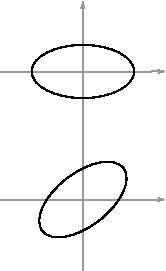
\includegraphics[width=0.3\textwidth]{images/fig_mc_detalle_elipses.pdf}
Eligiendo el punto $\phi_0 =0$ obtenemos una elipse como la de arriba.
}
Luego podemos utilizar $r_m, r_M$ lo cual determina $U_m, U_M$ respectivamente, cuyos valores son 
\[
	U^M_m = \frac{km}{L^2} \left( 1 \pm \sqrt{1 + \frac{2EL^2}{k^2 m} }\right)
\]
y esto nos permite fijar $A$. Incorporando esto en \eqref{sol_general} y recordando que $U(\phi) =1/r$ 
se tiene 
\[
	\frac{1}{r} = \frac{km}{L^2}\left( 1 +  \sqrt{1 + \frac{2EL^2}{k^2 m} } \cos( \phi ) \right),
\]
que no es otra cosa que la ecuación de una elipse en coordenadas polares con origen en un foco.
Veámoslo.

% \[
% 	\frac{1}{r} = \frac{km}{L^2} +  A \cos( \phi -\phi_0 )
% \]
% y habría que usar $r_m, r_M$ para evaluar $A$.

Las elipses verifican 
\[
	\frac{x^2}{a^2} + \frac{y^2}{b^2} = 1	\qquad \sigma^2 = a^2 - b^2
\]
donde $\sigma$ es la semi-distancia focal. Definiendo $ \sigma/a \equiv \varepsilon$ (la excentricidad) 
se puede expresar
\[
	b = a \sqrt{ 1 - \varepsilon^2 }
\]
\notamargen{Falta el sistema de coordenadas en el foco $f'$. Revisar quién es $EL$.}
\begin{figure}[hbt]
	\begin{center}
	\includegraphics[width=0.4\textwidth]{images/fig_mc_elipse_1.pdf} \hspace*{2em}	 
	\includegraphics[width=0.4\textwidth]{images/fig_mc_elipse.pdf}	 
	\end{center}
	\caption{}
	\label{fig_mc_elipse}
\end{figure} 

Por otro lado, usando el teorema del coseno para el triángulo definido en la Figura \ref{fig_mc_elipse} es 
\[
	s^2 = (2\sigma)^2 + r^2 - 4\sigma r \cos( \pi - \phi )
\]
y como $s+r$ es la distancia que se mantiene constante e igual, entre otras, a $2a$ se sigue que 
\[
	( 2a -r )^2 = 4\sigma^2 + r^2 + 4\sigma r \cos(\phi)
\]
cuya simplificación conduce a
\[
	\frac{1}{r} = \frac{1 + \varepsilon \cos (\phi)}{a(1-\varepsilon)} = \frac{a}{\phantom{^a}b^2} \left( 1 + 
\varepsilon \cos (\phi) \right)
\]
la cual es la ecuación de una elipse.

\notamargen{Acá hay que hacer un laburo muy importante.}
% \begin{figure}[hbt]
% 	\begin{center}
% 	\includegraphics[width=0.4\textwidth]{images/fig_mc_elipse.pdf}	 
% 	\end{center}
% 	\caption{}
% \end{figure} 

Entonces en resumen, las leyes de Kepler son
\begin{enumerate}
 \item Los planetas giran en órbitas elípticas con el Sol en uno de sus focos. Esto es común de los potenciales del 
tipo 
	\[
		V \propto 1/r
	\]
 \item El radio vector recorre áreas iguales en tiempos iguales
	\[
		\delta A = \frac{1}{2} r^2 \delta \phi \quad \longrightarrow \quad \dtot{A}{t} = \frac{r^2}{2} 
\dot{\phi} = \frac{L}{2m} (cte.)
	\]
	Esto es una característica de todo potencial central.
 \item El cubo del semieje mayor de la órbita de un planeta es proporcional al cuadrado del período empleado en 
recorrerla.
	La ecuación anterior, que da la velocidad areolar, se puede integrar como 
	\[
		\int dA  = \frac{L}{2m} \int dt
	\]
	que conduce a 
	\[
		\pi a b = \frac{L}{2m} \tau \qquad \longrightarrow \qquad a = \frac{L\tau}{2\pi b m}, 
	\]
	y luego, como $k m /L ^2 = a/b^2$ llegamos a 
	\[
		a^3 = \frac{k}{m} \frac{1}{4\pi^2} \: \tau^2 = \frac{GM}{4\pi^2} \tau^2
	\]
 y esto es independiente de la masa del planeta.
 
Como $a$ depende de $L$ se tiene que dependiendo de la energía $E$ tendré órbitas como las ilustradas debajo
todas las cuales tienen la misma energía 
\[
	a = \frac{1}{2}(r_M + r_m) = -\frac{k}{2E}
\] 

\includegraphics[scale=0.3]{images/fig_mc_orbitas_elipticas.jpg}

\notamargen{Esto estaba en la carpeta pero no lo entiendo bien del todo. Tal vez ilustración de la elipse con 
el sistema coordenado en el origen.}
 Para una elipse con el sistema coordenado en el centro se tiene 
 \[
	\frac{1}{r^2} = \frac{1}{b^2}( 1-\varepsilon^2 \cos^2 (\phi) )
 \]
 
\includegraphics[scale=0.3]{images/fig_mc_orbitas_elipticas_2.jpg} 
 
 Trabajamos más con la elipse,
 \[
	r_M + r_m = 2a
 \]
 \[
	E = \frac{L^2}{2mr^2} - \frac{k}{r}	\qquad\qquad E - \frac{L^2}{2m} U^2 - kU = 0
 \]
 \[
	\frac{1}{r_{m,M}} = \frac{ \frac{2mkE}{L^2} \mp \sqrt{ \left(\frac{2mkE}{L^2}\right)^2 + \frac{8mE}{L^2} } }{2}
 \]
 \[
	\frac{1}{r_{m,M}} = \frac{mEk}{L^2} \left( 1 \pm \sqrt{1 - \frac{2L^2}{mEk^2}}\right) 
 \]
 y acá constatamos que representa una elipse; es decir que las órbitas son elípticas.
\end{enumerate}

\begin{ejemplo}{\bf Problema 1 de central forces}

Conviene pasarlo a un problema equivalente para una partícula {\it masa reducida} en términos del centro de masa.
\[
	E = \frac M 2 V_{cm}^2 + \frac \mu 2 ( \dot{r}^2 + r^2\dot{\theta}^2 ) + V( r )
\]
\[
	\tau = \frac{2\pi R}{R\dot{\theta}}
\]

\includegraphics[scale=0.4]{images/fig_mc_central_forces1.jpg}

\[
	E = \frac 1 2 \mu(\dot{r}^2 + r^2\dot{\theta}^2 ) + \frac K r
\]
Al detenerlas,
\[
	E = - \frac K r
\]
y al rearrancar
\[
	E = \frac 1 2 \mu \dot{r}^2 - \frac K r
\]
\includegraphics[scale=0.4]{images/fig_mc_central_forces2.jpg}

Para la integración le pongo el signo negativo puesto que corresponde a la situación física correcta
\[
	\dtot{r}{\tau} = -\sqrt{ \frac 2 \mu \left(E + \frac K r \right) }
\]
Integración a ambos miembros lleva a
\[
	\int_0^\tau dt = - \int_R^0 \frac{dr}{ \sqrt{ \frac 2 \mu \left(E + \frac K r \right) } }
\]
o bien a 
\[
	\tau' = \sqrt{\frac{\mu}{2}} \sqrt{\frac{R}{K}} \int_R^0 \sqrt{\frac{r}{R-r}} dr
\]

Con el cambio de variables $U=\sqrt{R-r}$ que lleva al diferencial 
\[
	dU = \frac{-dr}{2\sqrt{R-r}}
\]
la integral resulta en 
\[
  	2 \left( \frac{ \mu R }{ 2K } \right) \int_0^{\sqrt{R}} \sqrt{ R - U^2 } dU =
 	2 \left( \frac{\mu R}{2K}\right) \left( \frac{ U\sqrt{R-U^2} }{2} + \frac{R}{2} 
 	\asen\left( \frac{U}{\sqrt{R}}\right) \right)
\]
que se ha buscado en tablas.
Luego,
\[
	\tau' = \sqrt{ \frac{\mu R}{2K} }\frac{R\pi}{2}
\]
y las ecuaciones de Newton,
\[
	\frac{K}{R^2} = \mu R\dot{\theta}^2 
\]
de la cual se puede despejar $\dot{\theta}$ para obtener
\[
	\tau = 2 \pi R \sqrt{\frac{\mu R}{K}}
\]
de manera que 
\[
	\frac{ \tau }{ \tau' } = 4 \sqrt{ 2 }.
\]
\end{ejemplo}

\begin{ejemplo}{\bf Problema 4 de central forces}

Consideramos un potencial de la forma 
\[
	V(r) = \frac{K}{r^2}
\]
que es un potencial repulsivo puesto que 
\[
	F(r) = -\dpar{V}{r} = \frac{2K}{r^3}
\]
implica que {\it aleja a la partícula}.
Como es central, conserva $ L = m r^2 \dot{\theta} $ se puede escribir la energía como
\[
	E = \frac 1 2 m ( \dot{r}^2 + r^2 \dot{\theta}^2 ) + \frac K {r^2} = \frac{ m \dot{r}^2 }{2} +
	\left( \frac{ \ell }{ 2 m r^2 } + \frac{ K }{ r^2 } \right)
\]

\includegraphics[scale=0.3]{images/fig_mc_potencial_central_4.jpg}

Luego,
\[
	\dot{r} = \sqrt{ \frac{2E}{m} - \frac{2L}{2m^2r^2} - \frac{2K}{mr^2} }
\]
y entonces
\[
	m r^2 \sqrt{ \frac{2E}{m} - \frac{2L}{2m^2r^2} - \frac{2K}{mr^2} } \dtot{\theta}{r} = L
\]
de manera que 
\[
	\int_0^{\theta} d\theta = \frac{L}{\sqrt{2m}} \int_{r_0}^{r} \frac{dr}{r^2( E - L/(2mr^2) - K/r^2 )^{1/2}}
\]

Con el cambio de variables $ U = 1 / r $
\[
	\theta = -\frac{L}{\sqrt{2m}} \int_{1/r_0}^{1/r} \frac{ dU }{ [ E - U^2( L/(2m) + K )]^{1/2} }
\]

Integrada da
\[
	\theta = \frac{L}{m\sqrt{2Km + \frac{L^2}{m^2}}}
	\left( \acos\left[ \frac{ \sqrt{2Km + L^2/(m^2)} }{r_0\sqrt{2E/m}} \right] - 
	\acos\left[ \frac{\sqrt{2Km + L^2/(m^2)}}{r\sqrt{2E/m}}\right] \right).
\]

Tomo $r_0$ punto de retorno
\[
	E = \left( \frac{L^2}{2mr_0^2} + \frac{K}{r_0^2} \right)
\]
y entonces
\[
	r_0 = \sqrt{ \frac L {2mE} + \frac K E }
\]
\[
	\theta = \frac{L}{m\sqrt{2Km + \frac{L^2}{m^2}}} \acos\left(\frac{r_0}{r}\right)
\]
y se puede despejar
\[
	r = \frac{ r_0 }{\cos( \theta m / L \sqrt{ 2 m K + L^2 / m^2 } )}
\]
\includegraphics[scale=0.3]{images/fig_mc_potencial_central_4_orbitas.jpg}

Continuamos con el problema [esto sacarlo, je!]

\includegraphics[scale=0.3]{images/fig_mc_potencial_central_5_orbitas.jpg}
\[
	r = \frac{ r_0 }{ \cos( \vp \sqrt{ 2 m^3 K / L^2 + 1 } ) }
\]
\notamargen{Ojo, chequear esta expresión porque en la carpeta está distinta!}

Vemos el comportamiento asintótico, si $ K = 0 $ entonces
\[
	r = \frac{ r_0 }{ \cos \vp }.
\]
Si el potencial es atractivo, por ejemplo $ V(r) = -\frac{K}{r^2}$ entonces se puede escribir 
\[
	E = \frac{1}{2} m \dot{r}^2 + \frac{K'}{r^2},
\]
donde 
\[
	K' = \left( \frac{L^2}{2m} - \frac{K}{} \right).
\]
Entonces la velocidad será 
\[
	\dot{r} = \sqrt{ \frac{2}{m}\left( E - \frac{K'}{r^2} \right) }
\]

A partir de la ecuación para el momento angular, $ m r^2 \dot{\vp} = L $ podemos llegar a la integral para $\vp(r)$ [esto creo que ya se hizo en la 
teoría, en dicho caso citar, sino hacer en detalle]
\[
	\int d\vp = \int \frac{L}{m} \frac{ dr }{ r^2 \sqrt{ \frac{2}{m}\left( E - \frac{K'}{r^2} \right) }}
\]
Con el reemplazo usual $r = 1/U$ se llega a 
\[
	\vp = -L \int \frac{ dU }{ ( 2mE - K'mU^2 )^{1/2}}.
\]

Si $L^2 > 2mK$ es 
\[
	\frac{L^2 - 2mK}{2m} > 0 \qquad K'>0
\]
y tengo un caso similar al anterior (en la página precedente[sic carpeta?]). En cambio si $ L^2 < 2mK $ se tiene $ K' < 0 $.
Usano la ayuda para la integral [refiere al enunciado en la guia?] que se hace entre $r_0$ y algún $r$ final resulta 
\[
	\vp =  \frac{L}{\sqrt{-2mK'}} \log \left( \frac{-2mE}{ \sqrt{ -2mK'/r } + \sqrt{2mE - K'/r^3} }\right)
\]
y esto dice que la partícula cae al origen describiendo una espiral. En el origen es $\dot{\vp} \to \infty$

\includegraphics[scale=0.3]{images/fig_mc_potencial_central_6_orbitas.jpg}

Dicho esto, se puede calcular el tiempo que tarda en caer al origen a partir de la ecuación para $\dot{r}$
\[
	-\int_{r_0}^0 \frac{1}{\sqrt{ 2/m ( E - K'/r^2 ) }} = \int_0^{t_f} dt
\]
Como la energía se conserva puede utilizarse su valor inicial, $E=K'/r_0^2$ de modo que el LHS de la ecuación anterior es
\[
	t_f = -\sqrt{ \frac{m}{-2K'} } \int_{r_0}^0 \frac{ r_0 r }{\sqrt{ r_0^2 - r^2 }} = r_0^2 \sqrt{\frac{m}{-2K'}}.
\]
\end{ejemplo}

% =================================================================================================
\section{Teorema del virial}
% =================================================================================================

Se aplica a sistemas de muchas partículas. Defino 
\[
	G \equiv \vb{p}_i \cdot \vb{x}_i
\]
de modo que como $ \dot{\vb{p}}_i = \vb{F}_i $ se tiene 
\[
	\dtot{G}{t} = \dtot{\vb{p}_i}{t} \cdot \vb{x}_i + \vb{p}_i \dtot{\vb{x}_i}{t}
\]
y se puede ver que el último miembro del RHS es $ \vb{p}_i \dot{\vb{x}}_i = m_i v_i^2 = 2T$ donde $T$ es la energía cinética del sistema.
Luego 
\[
	\dtot{G}{t} = \sum_i^N \dtot{\vb{p}_i}{t} \cdot \vb{x}_i + 2 T
\]

Defino el valor medio temporal de una cantidad $A$ según 
\[
	\bar{A} = \lim_{\tau \to \infty} \frac{1}{\tau} \int_0^\tau A(t) dt
\]
[Pasar esto a Apéndice!!].
\[
	\overline{G} = \frac{1}{\tau} \int_0^\tau \dtot{G}{\tau} dt = \overline{ 2 T } + \overline{ \sum_i^N \vb{F}_i \cdot \vb{x}_i }
\]
Pero el integrando en el LHS es un diferencial total, entonces 
\[
	\frac{1}{\tau} \left( G(\tau) - G(0) \right) = \overline{ 2 T } + \overline{ \sum_i^N \vb{F}_i \cdot \vb{x}_i }
\]

Si ahora estoy trabajando con un sistema que realiza un movimiento períódico, entonces en $\tau$ definido como ese período tiene 
\[
	\overline{ 2 T } + \overline{ \sum_i^N \vb{F}_i \cdot \vb{x}_i } = 0
\]
lo cual lleva a el teorema del virial\index{Virial, teorema del}
\[
	\overline{ T }  = - \frac{1}{2} \overline{ \sum_i^N \vb{F}_i \cdot \vb{x}_i }.
\]

También es cero si el mov. [?]

La temperatura media es 
\[
	\overline{T} = \frac 3 2 N k T'
\]
para partículas en un recipiente. La fuerza es por los golpeteos (la temperatura en realidad es microscópicamente una manifestación de golpeteo 
molecular). Si $ d\vb{F}_i = - p \hat{n}dA $ de modo que 
\[
	\frac{1}{2} \sum_i \vb{F}_i \cdot \vb{x}_i = -\frac{p}{2}\int_S \hat{n}\cdot\vb{x}dA =
	-\frac{p}{2} \int_V \nabla\cdot \vb{x} dV = - \frac{3}{2} p V
\]
y entonces, igualando con la expresión anterior de la $\overline{T}$ se tiene 
\[
	N k T = p V,
\]
que es la ecuación de estado del gas ideal.

Si ahora supongo $\vb{F} = -\nabla V$ homogénea de grado $k$
\[
	\overline{T} = -\frac{1}{2} \overline{ \sum_i^N \vb{F}_i \cdot \vb{x}_i } = 
	-\frac{1}{2} \overline{ \sum_i^N \dpar{V(\vb{x})}{\vb{x}_i} \cdot \vb{x}_i } = 
	\frac{1}{2} \overline{ k V(\vb{x} ) } = \frac{1}{2} k \overline{V}
\]
\notamargen{Acá hay que aclarar que hace la homogeneidad para transformar el gradiente en $kV$.}

Con un potencial central vale 
\[
	V = -\frac{C}{r} = -Cr^{-1},
\]
o sea que es un potencial homogéneo de grado $k=-1$. Entonces, para un movimiento periódico bajo una fuerza central,
será 
\[
	\overline{T} = -\frac{1}{2}\overline{V}
\]
de manera que $\overline{E} = \overline{T} + \overline{V} = 1/2 \overline{V}$. Para un oscilador armónico, como $k=-2$
se tiene $\overline{E} = 2\overline{T} = 2\overline{V} $



% =================================================================================================
\section{Vector de Runge-Lenz}
% =================================================================================================

Para el problema de Kepler también se conserva una cantidad llamada {\it vector de Runge-Lenz} definido como
\[
	\vb{R} = \vb{v} \times \vb{l} - \alpha \frac{\vb{x}}{x}.
\]

Luego, si le tomamos la derivada temporal, resulta
\[
	\dtot{\vb{R}}{t} = \left( \dtot{\vb{v}}{t} \times \vb{l} \right) + \left( \vb{v} \times \dtot{\vb{l}}{t} \right)
	- \alpha\frac{ \vb{v} }{x} + \frac{ \alpha }{x^2} \dtot{x}{t} \vb{x}
\]
donde el último se puede poner en términos de la velocidad si utilizamos la regla de la cadena así
\[
	\dtot{|\vb{x}|}{t} = \dtot{|\vb{x}|}{x_i} \dtot{x_i}{t} = \nabla( |\vb{x}| )\cdot \vb{v} \qquad  \qquad i=1,2,3
\]

Luego, cada componente $i$-ésimo del gradiente de la norma del vector de posición tiene (en coordenadas cartesianas) la 
misma
forma; tomando como ejemplo el $i=1$
\[
	\dtot{|\vb{x}|}{x_1} = \dtot{\sqrt{x_1^2 + x_2^2 + x_3^2}}{x_1} = \frac{x_1}{|\vb{x}|},
\]
de manera que 
\[
	\nabla( |\vb{x}| ) = \frac{\vb{x}}{x} = \hat{x},
\]
el gradiente de la norma del vector es su dirección. Entonces, volviendo a la ecuación original resulta 
\[
	\dtot{\vb{R}}{t} = \left( \dtot{\vb{v}}{t} \times \vb{l} \right) + \left( \vb{v} \times \dtot{\vb{l}}{t} \right)
	- \alpha\frac{ \vb{v} }{x} + \alpha \:\vb{x} \left( \frac{ \pe{x}{v} }{x^3}\right) 
\]

Dado que $\vb{l} = \vb{x} \times m \vb{v}$ el segundo término en la anterior expresión desaparece y nos queda
\[
	\dtot{\vb{R}}{t} = \left( \dtot{\vb{v}}{t} \times [ \vb{x} \times m\vb{v} ] \right) 
	- \alpha\frac{ \vb{v} }{x} + \alpha \:\vb{x} \left( \frac{ \pe{x}{v} }{x^3}\right) 
\]

\notamargen{Aparentemente esto tiene que dar nulo pero no lo estaría viendo.}

\[
	\dtot{\vb{V}}{t} \times ( \vb{x} \times m\vb{v} ) +
	\vb{V} \times \left( \dtot{\vb{r}}{t} \times m\vb{v} + \vb{r} \times m\dtot{\vb{v}}{t} \right)
\]
pero como $\dtot{\vb{r}}{t} \times m\vb{v} = 0$ resulta lo que resulta.
\begin{figure}[hbt]
	\begin{center}
	\includegraphics[width=0.4\textwidth]{images/fig_mc_rungelenz.pdf}	 
	\end{center}
	\caption{}
\end{figure} 

El vector de Runge-Lenz siempre apunta en la misma dirección dada su constancia (ver figura).
\notamargen{Mejorar la figura!}

Escribo $ T = E - V $
\[
	r_{max} m v^2 = 2Er_{max} + 2\alpha
\]
pero 
\[
	r_{max} = \frac{2 E l^2 \alpha}{\alpha^2 m (1-\varepsilon)} = \frac{-1}{\alpha}\frac{b^2 
\alpha}{\alpha^2(1-\varepsilon)}
\]
\[
	r_{max} = - (1+\varepsilon) \alpha
\]

\[
	b^2 = a^2( 1 - \varepsilon^2 )
\]

\begin{ejemplo}{\bfseries Vector de Runge-Lenz en órbitas elípticas}
\notamargen{Este título es provisorio. Está en la carpeta en 42R.}

Sabemos que el vector de Runge-Lenz tiene la forma 
\[
	\vb{A} = \pv{V}{L} - \alpha \frac{\vb{x}}{x}
\]
y cumple 
\[
	\dtot{A}{t} = 0
\]

Veamos qué expresión tiene el módulo $ A \equiv |\vb{A}| $. Tomando el producto escalar 
\[
	\pe{A}{x} = A r \cos \theta = ( \pv{V}{L} )\cdot \vb{x} - \alpha \frac{\pe{x}{x}}{x}
\]
y reescribiendo (ciclicidad del producto vectorial)
\[
	( \pv{V}{L} )\cdot \vb{x} = \vb{L} \cdot ( \pv{r}{v} ) = \vb{L} \cdot \frac{ \vb{L} }{m} = \frac{L^2}{m}
\]
y entonces
\[
	\alpha r \left( 1 + \frac{A}{\alpha} \cos \theta \right) = \frac{L^2}{m}
\]
pero como $ (1 + \varepsilon \cos \theta ) = p / r $ es la excentricidad se tiene $ A = \varepsilon \alpha $.

\end{ejemplo}

\begin{ejemplo}{\bf Problema . Nuevo potencial}

Para el potencial 
\[
	U(r) = -\frac{\alpha}{r} + \delta U(r), \qquad |\delta U| \ll \frac{\alpha}{r}
\]
la integral resultante es
\[
	\vp = \int \frac{L dr }{r^2\sqrt{2m(E-U)-\frac{L^2}{r^2}}}
\]
pero si derivamos con respecto a un parámetro (por ejemplo $L$) se pueda cambiar la misma a 
\[
	\vp = - \dtot{}{L} \int \frac{ \sqrt{2m(E-U)- L^2} }{r^2}dr
\]
y esta segunda se comporta mejor que la primera.

\includegraphics[scale=0.35]{images/fig_mc_potencial_central_problema.jpg}

Una órbita no cerrada, a la larga, pasas por todos los putnos dentro del área barrida.

Ahora se trabajará el integrando anterior
\[
\sqrt{ 2m \left(E+ \frac{\alpha}{r}\right) - 2m\delta U - \frac{L^2}{r^2} } =
\sqrt{ 2m \left(E+ \frac{\alpha}{r}\right) - \frac{L^2}{r^2} } 
\sqrt{ 1 - \frac{ 2m\delta U }{ 2m \left(E+ \frac{\alpha}{r}\right) - \frac{L^2}{r^2} }  }
\]

Se puede considerar una expansión de Taylor en la segunda raíz de manera que 
\[
	\vp = - \dtot{}{L}\left[ \int 
	\sqrt{ 2m \left(E+ \frac{\alpha}{r}\right) - \frac{L^2}{r^2} } dr -
	m \int \frac{ \delta U dr }{ \sqrt{ 2m \left(E+ \frac{\alpha}{r}\right) - \frac{L^2}{r^2} }  }
	\right]
\]
\[
	\vp = 2 \pi + m \dtot{}{L} 
	\int \int \frac{ \delta U dr }{ \sqrt{ 2m \left(E+ \frac{\alpha}{r}\right) - \frac{L^2}{r^2} }  }
\]
donde el primer resultado, $2\pi$, proviene de la solución del problema de Kepler y el segundo es 
un término $\Delta \vp$ que dependrá de la forma de la perturbación.
Considerando perturaciones del tipo
\[
	\delta U = \frac{\beta}{r^2} \qquad \qquad \delta U = \frac{\gamma}{r^3}
\]

Antes de proceder es conveniente hacer un pasaje de la integral. Recordando que se tenía
\[
	dt = \frac{dr}{ \sqrt{ 2m \left(E+ \frac{\alpha}{r}\right) - \frac{L^2}{r^2} } }
\]
y que la conservación del momento angular $L$ implicaba
\[
	L = mr^2\dot{\theta}{t},
\]
si pasamos $\theta$ a $\vp$ entonces $dt = ( mr^2/L ) d\vp $ y consecuentemente
\[
	m r^2 d\vp = \frac{ L dr }{ \sqrt{ 2m \left(E+ \frac{\alpha}{r}\right) - \frac{L^2}{r^2} } }
\]
de forma que 
\[
	\Delta \vp = \dtot{}{L} \left( \frac{m^2}{L} \int_0^{2\pi} \delta U r^2 d\vp \right).
\]

Regresando ahora a las formas específicas planteadas, vemos que en el primer caso es
\[
	\Delta \vp = \beta m^2 2 \pi \dtot{}{L}\frac{1}{L} = - \frac{2\pi m^2 \beta}{L^2},
\]
mientras que para el segundo la integral resulta en
\[
	\gamma \int_0^{2\pi} \frac{d\vp}{r(\vp)}, 
\]
que se puede hacer explícitamente recordando que $p = L^2/(m\alpha)$ y
\[
	\frac p r = 1 + \varepsilon \cos \vp
\]
y entonces 
\[
	\frac 1 r = \frac{m\alpha}{L^2} + \frac{\varepsilon \cos \vp}{L^2},
\]
todo lo cual lleva a que 
\[
	\Delta \vp = \dtot{}{L}\left( \frac{m^3}{L^3} \gamma \alpha \right) =
	-\frac{3m^2\gamma \alpha}{L^4}.
\]
\end{ejemplo}

% =================================================================================================
\section{Precesión [acomodar]}
% =================================================================================================

Este movimiento, ver figura, corresponde a una oscilación completa de $r_m$ a $r_M$ y vuelta.
La precesión de un punto de la órbita se aplica a órbitas en las cuales puede pensarse que la órbita se mueve 
como un todo en su figura. La magnitud $\delta \vp / \tau_r$ es la velocidad angular de precesión.

\[
	\mbox{ Ilustración 45R inferior }
\]

% =================================================================================================
\section{Orbitas de potenciales centrales}
% =================================================================================================

\[
	V(r) = -\frac{\alpha}{r}
\]
\[
	V(r) = \frac{ k r^2 }{2}
\]
Estos dos casos dan órbitas cerradas. Pero hay otros potenciales interesantes.
El potencial de Yukawa
\[
	V(r) = - \frac{\euler^{-\lambda r}}{r^\alpha}
\]
que es aproximadamente como un potencial coulombiano apantallado ($\alpha=1,\lambda=0$).
Otro es el oscilador no armónico\index{Oscilador no armónico}
\[
	V(r) = r^\alpha
\]
Algunos casos se muestran bajo estas líneas

\begin{figure}[hbt]
	\begin{center}
	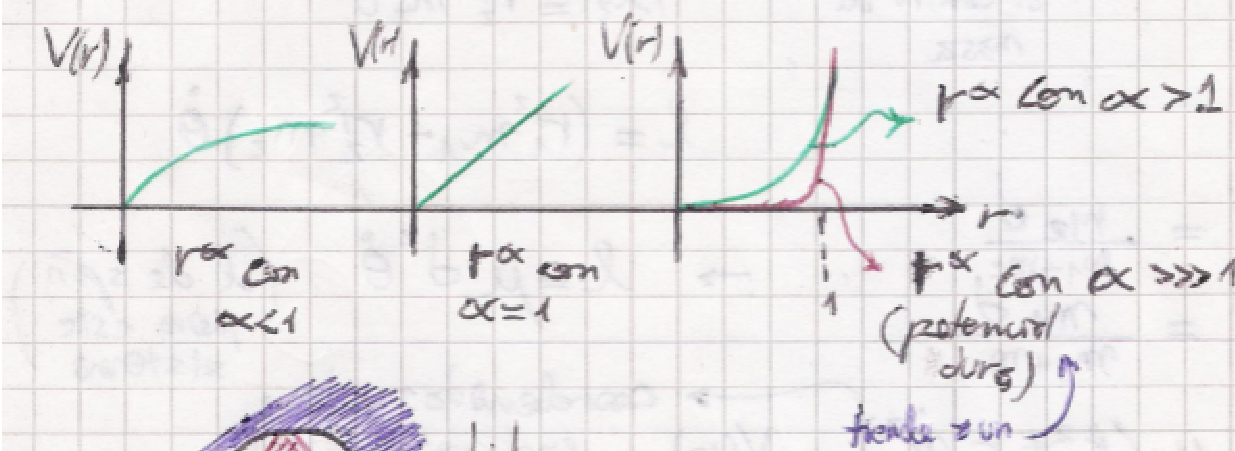
\includegraphics[width=0.6\textwidth]{images/fig_mc_potenciales_otro.pdf}
	\end{center}
	\caption{Algunas curvas de potenciales anarmónicos $ r^\alpha $.}
\end{figure}

Da órbita que no se cierra en un billar elíptico.

\begin{figure}[hbt]
	\begin{center}
	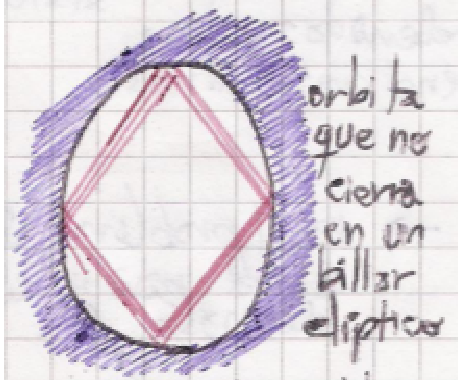
\includegraphics[width=0.4\textwidth]{images/fig_mc_billar.pdf}
	\end{center}
	\caption{.}
\end{figure}

% =================================================================================================
\section{Reducción del problema de dos cuerpos a uno equivalente}
% =================================================================================================

Para dos partículas de masas $ m_1 $ y $ m_2 $ sometidas a una fuerza central 
\[
	\vb{F}_{21} = F(r) \hat{r}_{21} \qquad \qquad F(r) = -\dtot{V(r)}{r}
\]
siendo $x \equiv |\vb{x}_2-\vb{x}_1|$ la distancia relativa.

\begin{figure}[hbt]
	\begin{center}
	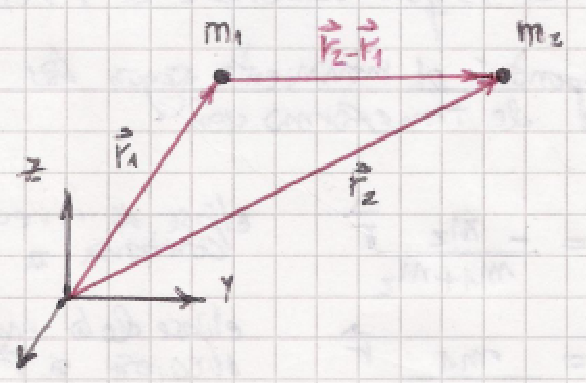
\includegraphics[width=0.4\textwidth]{images/fig_mc_prob_equiv_scheme.pdf}	 
	\end{center}
	\caption{.}
	\label{fig_mc_prob_equiv_scheme}
\end{figure} 

La energía del sistema será de la forma  $ E = T_1 + T_2 + V(r) $ pero se puede expresar según 
$ E = T_{cm} + T_{rel} + V(r) $; es decir separando la energía cinética en el aporte del centro de
masa más un aporte que depende de la distancia relativa entre los cuerpos.
De modo idéntido para el momento angular podemos pasar de $ L_{total} = L_{cm} + L_{spin} $ donde el
momento angular de spin es el referido al movimiento en torno al centro de masas.

\notamargen{Revisar y consolidar toda la notación aquí, que está mezclada.}
Consideramos el siguiente sistema de coordenadas,
\[
	r \equiv | \vb{r}_2 - \vb{r}_1 | \qquad	\qquad  \dot{r} \equiv | \dot{\vb{r}}_2 - \dot{\vb{r}}_1 |
\]
donde el sistema centro de masas es
\[
	\vb{R}_{cm} = \frac{ m_1\vb{r}_1 + m_2\vb{r}_2 }{ m_1 + m_2 }	\qquad 
	M \vb{V}_{cm} =  m_1\vb{v}_1 + m_2\vb{v}_2 
\]
\[
	0 = m_1\vb{r}_1' + m_2\vb{r}_2'
\]
que provocan
\[
	\vb{r}_1' = -\frac{m_2}{m_1}\vb{r}_2' \qquad   \vb{r}_2' = -\frac{m_1}{m_2}\vb{r}_1' 
\]
dando unas $r$ relativas
\be
	\vb{r} = \vb{r}_1' - \vb{r}_2' = -\frac{ m_1 + m_2 }{ m_1 } \vb{r}_2' = -\frac{ m_1 + m_2 }{ m_2 } \vb{r}_1'.
	\label{r_relativas}
\ee

\begin{figure}[hbt]
	\begin{center}
	\includegraphics[width=0.4\textwidth]{images/fig_reduccion.pdf}	 
	\end{center}
	\caption{Sistema coordenado para la reducción del problema de dos cuperpos al de uno equivalente.}
\end{figure} 

Luego, como la energía se conserva (el $V_{cm}=cte.$) podemos escribir
\[
	E = \frac{1}{2} m_1 \dot{\vb{r}}_1^2 + \frac{1}{2} m_2 \dot{\vb{r}}_2^2 + V(r)
\]
\[
	E = \frac{1}{2} m_1 ( \dot{\vb{R}} + \dot{\vb{r}}_1' )^2 + \frac{1}{2} m_2 ( \dot{\vb{R}} + \dot{\vb{r}}_2' )^2 
+ V(r)
\]
\[
	E = \frac{1}{2} m_1 ( {\vb{V}} )^2 +  \frac{1}{2} m_1 ( \dot{\vb{r}}_1' )^2 + 
		\frac{1}{2} m_2 ( {\vb{V}})^2 + \frac{1}{2} m_2 (\dot{\vb{r}}_2' )^2 + V(r)
\]
\[
	E = \frac{1}{2} M {\vb{V}}^2 + \frac{1}{2} \frac{m_2^2}{m_1} \dot{\vb{r}}_2'^2 + \frac{1}{2} m_2 
\dot{\vb{r}}_2'^2 + V(r)
\]
\[
	E = \frac{1}{2} M {\vb{V}}^2 + \frac{1}{2} \frac{m_2 m_1}{M} \dot{\vb{r}}^2 + V(r).
\]

Pero como $E$ y la $\vb{V}$ se conservan, se tiene 
\[
	e \equiv E - \frac{1}{2} M {\vb{V}}^2 =  \frac{1}{2} \mu \dot{\vb{x}}^2 + V(r)
\]
donde $e$ es una cantidad conservada que podemos llamar la energía reducida[?].

Este último $\vb{x}$ es un vector distancia relativa. Es un problema equivalente para la partícula
centro de masas.

\begin{figure}[hbt]
	\begin{center}
	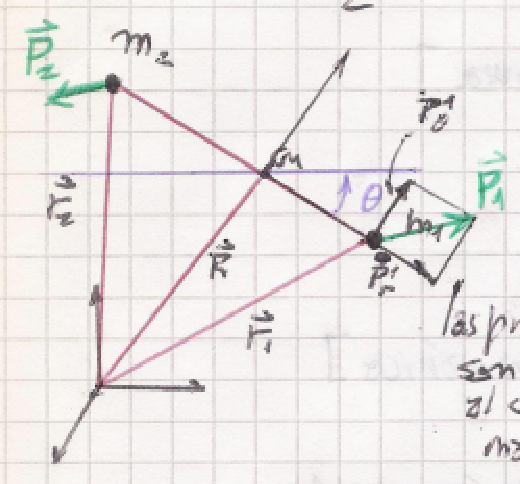
\includegraphics[width=0.4\textwidth]{images/fig_mc_prob_equiv.pdf}	 
	\end{center}
	\caption{.}
	\label{fig_mc_prob_equiv}
\end{figure} 

Podemos considerar ahora los momentos angulares de las partículas respecto de este sistema centro
de masas. Así
\[
	\vb{l}_1' = \vb{x}_1' \times \vb{p}_1 \qquad \qquad  \vb{l}_2' = \vb{x}_2' \times \vb{p}_2'
\]
y sus módulos verifican 
\[
	|\vb{l}_1'| = {x}^{2'}_1 m_1 \dot{\theta} \qquad \qquad  |\vb{l}_2'| = {x}^{2'}_2 m_2 \dot{\theta}
\]
de manera que 
\be
	\ell = ( {x}^{2'}_1 m_1 + {x}^{2'}_2 m_2 ) \dot{\theta} = \mu r^2 \dot{\theta}
	\label{mom_ang_conserv}
\ee
es el momento angular de spín para este sistema. Nótese que a partir de \eqref{r_relativas} se puede
expresar las $x'_i$ ($i=1,2$) en términos de $r$.

Luego, en coordenadas polares en el centro de masa resulta
\[
	e = \frac{1}{2} \mu ( \dot{ r}^2 + r^2\dot{\phi}^2 ) + V(r),
\]
o bien, usando \eqref{mom_ang_conserv},
\[
	e = \frac{1}{2} \mu \dot{ r}^2 + \frac{\ell^2}{2 \mu r^2 } + V(r)
\]
que no es otra cosa que el problema de fuerza central para un cuerpo de masa $\mu$.

Diremos que la {\it distancia relativa} describe una elipse. Las trayectoria reales en el espacio físico
son dos elipses confocales. Por supuesto dejan de cumplirse las leyes de Kepler en este caso.

Si como solución proponemos
\[
	V(r) = -\frac{\alpha}{r}
\]
tendré $ r = r(\phi) $ una elipse, que es lo que describe el $ r $ relativo.
Se descompondrá el movimiento según las ecuaciones de transformación
\[
	\vb{r}_1'= -\frac{m_2}{m_1+m_2} \vb{r} \qquad \text{ Elipse de dirección contraria a $\vb{r}$}
\]
\[
	\vb{r}_2'= \frac{m_1}{m_1+m_2} \vb{r} \qquad \text{ Elipse de dirección igual a $\vb{r}$}	
\]
Tendremos dos elipses confocales como muestra la figura bajo estas líneas 

\begin{figure}[hbt]
	\begin{center}
	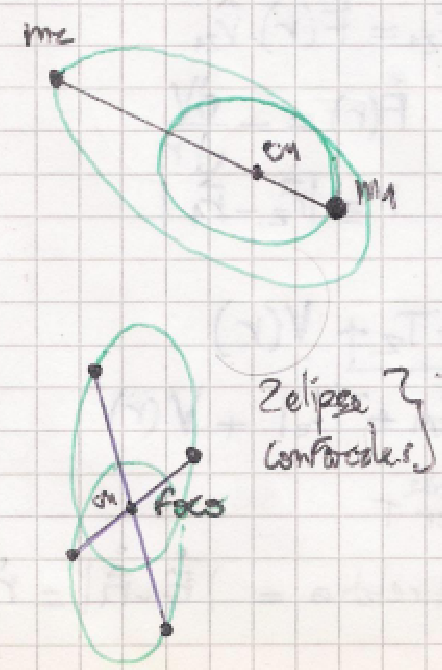
\includegraphics[width=0.4\textwidth]{images/fig_mc_elipses_confocales.pdf}	 
	\end{center}
	\caption{.}
	\label{fig_mc_elipses_confocales}
\end{figure} 

En este caso ya dejan de cumplirse las leyes de Kepler
\[
	\dtot{\mathcal{A}}{t} = \frac{\ell}{2\mu} \qquad a^3 \sim \tau^2 
\]
para la órbita relativa.
\[
	\frac{\pi a b }{\tau}= \frac{\ell}{2\mu} 
\]
\[
	b = \frac{\ell}{\sqrt{\alpha \mu}} a^{1/2} \qquad \frac{a}{b} = \frac{\mu \alpha}{\ell^2}
\]
\[
	\frac{\pi a^{3/2}}{\sqrt{\alpha \mu} \tau} = \frac{1}{2\mu}
\]
y entonces ahora se ve que no es independiente de las masas y no se puede simplificar $\sqrt{\mu\alpha}$ con
$\mu$ como ocurría en un movimiento elíptico tradicional (bajo potencial gravitatorio).
Entonces no es válida la ley de Kepler.

% =================================================================================================
\section{Dispersión}
% =================================================================================================

\subsection{preliminares--usar y destruir--}

Se supone una partícula chocando a la vez (el haz incidente no interactúa entre sí).
Se conoce las partículas incidentes por área y por tiempo $I$ y las dispersadas serán
$ D = I \int \dtot{\sigma}{\Omega} d\Omega = I \sigma$.
Se consideran coordenadas en el centro de masa.
Se trabaja en ángulos sólidos.
\notamargen{El problema 1 en página 45 parece estar hecho en la teoría, de manera que no transcribe
ahora.}

\includegraphics[scale=0.3]{images/fig_mc_dispersion_varios.jpg}

Es un tema muy importante porque permite investigar qué hay en el interior de la materia por medio
de {\it pegarle} con algo que se conoce perfectamente.
En estas situaciones el blanco es desconocido y el proyectil conocido.

Pero proyectil y blanco pueden actuar de acuerdo a un potencial. Esta interacción queda especificada
por la {\it sección eficaz de dispersión elástica}.

Veamos primeramente a lo que se llama un {\it centro dispersor} (blanco de masa tendiendo a infinito).
Al lanzar un haz de partículas (proyectiles) en primera instancia están libres y al acercarse recién se
notan los efectos.

Consideramos la dispersión de un haz de partículas de cierta energía cinética por un centro dispersor,
ver ilustración. Todas las partículas tienen la misma energía $1/2 m V_\text{ cm }$

\begin{figure}[htb]
	\begin{center}
	\includegraphics[width=0.5\textwidth]{images/fig_mc_dispersion1.pdf}	 
	\end{center}
	\caption{}
\end{figure} 


La sección eficaz diferencial es $d\sigma$ que es el número de partículas dispersadas entre 
$\chi$ y $\chi + d\chi$ por unidad de tiempo.
Pero esto depende del ancho del haz y de la cantidad de partículas del haz. Para independizarlo se
divide por la intensidad del haz (\# de partículas por área) y se construye así $d\sigma'$
\[
	d\sigma' \equiv \dtot{\sigma}{n} dA dt 
\]
y así $d\sigma'$ tiene unidades de área. Obviaremos en lo que sigue la ``''' en la notación.
Entonces, ahora, la sección eficaz diferencial, bien definida, es 
\[
	d\sigma = \frac{dN}{n}
\]
siendo $dN$ el número de partículas dispersadas entre $\chi$ y $\chi + d\chi$ por unidad de tiempo
y $n$ el número de partículas emitidas por tiempo y por área.

Si el centro dispersor tiene simetría esférica el cálculo es sencillo, puesto que se conserva el 
momento angular $L$. En realidad, ya con la simetría radial cilíndrica en torno a la dirección del 
haz basta para resolver analíticamente.
Estas suposiciones son muy fuertes y restrictivas pero a fin de cuentas este es un caso de gabinete
para formar algunas ideas.

Consideramos $d$ centro dispersor con simetría esférica (cilíndrica basta).

\[
	mbox{ \text{ Figura 46 abajo. } }
\]

Usamos como suposiciones que todo lo que emerge entre $\rho + d\rho$ - $\rho$  es dispersado entre
$\chi + d\chi$ - $\chi$, y que se conservan tanto $E$ como \vb{L}.

\begin{figure}[htb]
	\begin{center}
	\includegraphics[width=0.5\textwidth]{images/fig_mc_dispersion2.pdf}	 
	\end{center}
	\caption{}
\end{figure}

El anillo se dispersa en un sector esférico. Entonces para el anillo entre $\rho + d\rho$ - $\rho$ el
área de la corona será
\[
	A =  \pi ( (\rho + d\rho)^2 - \rho^2 ),
\]
que a primer orden (suponiendo $d\rho$ diferencial) será 
\[
	A \approx 2 \pi \rho \: d\rho.
\]

La variable $\rho$ es el llamado {\it parámetro de impacto}. Entonces
\[
	d\sigma = \frac{  2 \pi \rho \: d\rho I}{I} = 2 \pi \rho d\rho
\]
donde $I$ el número de partículas por unidad de tiempo y área
en el haz. Si obtuviese $ \rho = \rho(\chi) $ entonces inalmente
\[
	d\sigma =  2 \pi \rho(\chi) \left| \dtot{\rho}{\chi} \right| d\chi
\]
donde el módulo es porque la cantidad correspondiente será negativa. La función $\rho(\chi)$ nos dará
información sobre el potencial entre las partículas y el centro.
La función $\chi(\rho)$ se llama función deflexión.

Como se conservan la energía y el momento angular
\[
	E = \frac{1}{2} m V_\infty^2 \qquad L = m \rho V_\infty^2 
\]
aunque por supuesto al variar $\rho$ varío el momento angular $L$ de las partículas. Entonces tanto una
como otra magnitud determinan cómo se dispersan las partículas.

La conservación de $L$ implica la constancia de $\rho$ como valor asintótico para la trayectoria. El punto
apsidal es un punto tal que existe simetría de la órbita respecto al mismo.
\[
	mbox{ \text{ figura 46R izquierda} }
\]
\begin{figure}[htb]
	\begin{center}
	\includegraphics[width=0.5\textwidth]{images/fig_mc_dispersion3.pdf}	 
	\end{center}
	\caption{}
\end{figure}

Se puede calcular el ángulo $\varphi_0$ de acuerdo a 
\[
	\chi = \pi - 2\varphi_0,
\]
donde
\[
	\varphi_0 = \int_{r_m}^{\infty} \frac{L/mr^2}{\sqrt{\frac{2}{m}(E - V_{\text{eff}} )}} dr
\]
\[
	\chi = \pi - 2 \varphi_0 (\rho)
\]
e invertimos desde la última ecuación. Considerando $E = 1/2 m v_\infty$ y $ L = m \rho v_\infty $
se tiene 
\[
	V_{\text{eff}} = \frac{L}{2 m r^2} + V(r)
\]
aunque en general se desconoce $V(r)$ o el tamaño efectivo de su interacción. En esos casos se puede 
ajustar el cálculo con lo que se mide experimentalmente para tener un potencial parecido a la interacción
real.

\subsection{Esfera maciza}

Veamos el caso de una esfera maciza. Lo primero es encarar el cálculo de $\rho=\rho(\chi)$ o su inversa.
En general los cuerpos duros equivalen a un potencial del tipo
\be
	V = \begin{cases}
	     \infty \qquad \textrm{cuerpo}\\
	     \;0 \qquad \; \textrm{fuera}
	    \end{cases}
	    \label{potencial_hard}
\ee
Si el potencial $V$ en la esfera no fuese infinito eso significa que hay partículas que podrían ingresar.

\[
	\mbox{ \text{ Figura 47 potenciales } }
\]


La geometría del problema es tal que 
\begin{figure}[htb]
	\begin{center}
	\includegraphics[width=0.5\textwidth]{images/fig_mc_dispersion4.pdf}	 
	\end{center}
	\caption{}
\end{figure}
\[
	\chi = \pi - 2\varphi_0
\]
\[
	\sin(\varphi_0) = \frac{\rho}{a} \qquad d\rho = -a \frac{1}{2}\cos \left(\frac{\pi-\chi}{2}\right)
\]
y entonces 
\[
	d\sigma = 2\pi a^2 \sin\left(\frac{\pi-\chi}{2}\right) \frac{1}{2}\cos\left(\frac{\pi-\chi}{2}\right) d\chi
\]
\[
	d\sigma = \frac{\pi}{2} a^2 \sin( \pi-\chi) d\chi = \frac{\pi}{2} a^2 \sin( \chi) d\chi
\]
y como hay que integrar $\chi$ de 0 a $\pi$
\[
	\int_0^\pi \frac{\pi}{2} a^2 \sin( \chi) d\chi = \pi a^2
\]
\[
	\sigma = \pi a^2
\]
En el caso de los cuerpos duros (potencial constante del tipo del dado en \eqref{potencial_hard}) la sección
eficaz total $\sigma$ es la sombra de los mismos.

\subsection{Ángulo sólido}

El ángulo sólido total para una esfera es $\Omega = 4 \pi $ y es igual a $A/r^2$ siendo $A$ el área de la
misma. El diferencial de ángulo sólido se construye a partir de la ilustración 
\[
	\mbox{ Figura 47 inferior dentro de inserto }
\]
y se ve que es 
\[
	d\Omega = 2 \pi \sin \chi d\chi.
\]
Luego, para la dispersión por una esfera,
\[
	d\sigma = \frac{a^2}{4} d\Omega,
\]
la sección eficaz diferencial es constante y la sección eficaz total (integrada) $\sigma = \pi a^2$ da
información sobre el número de partículas que se desvían. Podemos pensar que las partículas se desvían
si caen dentro del área de la {\it sombra} del blanco.

\[
	\mbox{ Figura 47 ultima, esfera con rayitos }
\]

\notamargen{Sobre el ángulo sólido
\[
\Omega = \textrm{Area}/r^2
\]
\[
d\Omega = 2 \pi \sin( \chi ) d\chi 
\]
\[
\Omega = 4 \pi 
\]
para la esfera.
}

\begin{ejemplo}{\bf Pozo esférico de profundidad $V_0$}
 
\[
	\mbox{ Figura 47R segunda, para el ejemplo. }
\] 
 
La geometría del problema implica que 
\[
	\chi = 2(\alpha - \beta)
\]
y la conservación de la energía,
\[
	E = \frac 1 2 m v_1^2 = \frac 1 2 m v_2^2 - V_0,
\]
implica que 
\[
	\frac {v_2} {v_1} = \sqrt{ 1 + \frac{V_0}{E}} \equiv n
\]
y entonces $ v_1 \sin \alpha = v_2 \sin \beta$ lo cual conduce a  
\[
	\frac{\sin \beta}{\sin \alpha} = \frac{\sin (\alpha - \chi/2 )}{\sin \alpha} = \frac 1 n
\]
y $\sin \alpha = \rho / a$.
La conservación del momento angular $\vb{L}$ determina que el trayecto rojo en la figura sea 
el que ocurre.

Supongamos que no hay conservación del momento angular, como en la situación ilustrada aquí abajo,
\[
	\mbox{ Figura 47R final final}
\]

Se tendrá entonces
\[
	\frac{\sin \gamma}{\sin \vp} = \frac{1}{\sqrt{ 1 + V_0/E }}
\]
aunque hay un ángulo (el de reflexión interna total) que hará que no salgan partículas puesto que 
son atrapadas por el cuerpo.

Existe un $\rho$ de rebote (de reflexión interna) y entonces $\chi=\chi(\rho)$ será discontinua a 
saltoss porque para un cierto $\rho$ sale y para un $\rho + d\rho$ ya no.

\[
	\mbox{ Figura 48 con toda la explicación }
\]
\notamargen{Hay unos comentarios jugosos respecto de esta figura que habría que explotar.}

Si el momento angular no se conserva no es posible calcular $\chi = \chi(\rho) $.
\end{ejemplo}


% =================================================================================================
\section{Dispersión por dos cuerpos}
% =================================================================================================

El problema de la dispersión de dos cuerpos se puede tratar en modo similar al de un cuerpo si se
convierte el mismo en un problema equivalente para un cuerpo de masa $\mu$.

Así la situación de dos cuerpos interactuando se convierte en la de un cuerpo por un potencial.
El asunto es que aquí varían los ángulos de dispersión porque estamos considerando un sistema
en el centro de masas.
\notamargen{Esto requerirá alguna ilustración visual.}

Sea una masa M que se fisiona en un punto por alguna interacción desconocida. Pensamos un haz de
estas partículas M que se fisionan del mismo modo.

\includegraphics[scale=0.3]{images/fig_mc_dispersion_2cuerpos1.jpg}

Desde el centro de masas se vería una situación como la mostrada en la ilustración

\includegraphics[scale=0.3]{images/fig_mc_dispersion_2cuerpos2.jpg}

La ilustración con coordenadas sería algo como:
\begin{figure}[htb]
	\begin{center}
	\includegraphics[width=0.5\textwidth]{images/fig_mc_disp2body1.pdf}	 
	\end{center}
	\caption{}
\end{figure} 

Desde el centro de masa se conserva el momento, y entonces
\[
	\vb{P}_1 + \vb{P}_2 = 0
\]
\[
	m_1 \vb{v}_1 + m_2 \vb{v}_2 = 0
\]
definimos una velocidad relativa
\[
	\vb{v} \equiv \vb{v}_2  - \vb{v}_1 = \vb{v}_2 \left( \frac{ m_1 + m_2 }{ m_1 }\right) .
\]
\begin{figure}[htb]
	\begin{center}
	\includegraphics[width=0.5\textwidth]{images/fig_mc_disp2body2.pdf}	 
	\end{center}
	\caption{}
\end{figure} 

Con respecto a la energía,
\[
	\frac{1}{2} M \vb{V}_{cm}^2 + e_{int} = \frac{1}{2} m_1 \vb{v}_1^2 + \frac{1}{2} m_2 \vb{v}_2^2
						+ e_{int 1 } + e_{int 2} + \frac{1}{2} M \vb{V}_{cm}^2
\]
\[
	\frac{1}{2} m_1 \vb{v}_1^2 + \frac{1}{2} m_2 \vb{v}_2^2 = e_{int} - e_{int 1 } - e_{int 2} = \Delta e
\]
y pasando todo en términos de la velocidad relativa
\[
	 \frac{1}{2} \frac{m_1 m_2}{ m_1 + m_2 } v = \Delta e
\]
entonces 
\[
	v = \sqrt{\frac{ 2 \Delta e}{ \mu } }.
\]

Como la velocidad relativa $v$ es una constante se sigue que la separación de los cuerpos es a
velocidad constante.
Por otra parte, la energía interna $e$ es la que provoca la fisión. Se puede pensar que existe un
resorte que {\it revienta} espontáneamente y separa ambas partículas.

\begin{figure}[htb]
	\begin{center}
	\includegraphics[width=0.5\textwidth]{images/fig_mc_disp2body3.pdf}	 
	\end{center}
	\caption{}
\end{figure} 

Conocemos el módulo de la velocidad pero no su dirección.
El problema es evidentemente plano. Consideramos que todo se mide desde el centro de masas y el
problema es no relativista.
Desde un sistema laboratorio 
\[
	\vb{V}_1^L =  \vb{V}_{cm} + \vb{V}_1' \qquad \longrightarrow \quad ( \vb{V}_1^L - \vb{V}_{cm} ) = \vb{V}_1'
\]
\[
	{V_1^L}^2 - V_{cm} - 2 {\vb{V}_1^L}^2 \vb{V}_{cm} = V_1^2
\]
\[
	{V_{1x}^L}^2 + {V_{1y}^L}^2 - V_{cm} - 2 {V_{1x}^L}^2 V_{cm} = V_1^2
\]
\[
	( V_{1x}^L  - V_{cm} )^2 + {V_{1y}^L}^2 = V_1^2
\]
que es una circunferencia en el plano.
De la ilustración puede verse que 
\[
	\tan(\theta) = \frac{V_1 \sin(\chi) }{ V_{cm} + V_1 \cos(\chi) }
\]
\begin{figure}[htb]
	\begin{center}
	\includegraphics[width=0.45\textwidth]{images/fig_mc_disp2body4a.pdf}	 
	\includegraphics[width=0.45\textwidth]{images/fig_mc_disp2body4b.pdf}
	\end{center}
	\caption{}
\end{figure} 

Luego, se puede despejar de la anterior ecuación el valor de $\chi$. Para ello se elevan
ambos miembros al cuadrado, se expande como 
\[
	\tan^2 \theta \left( \frac{V_{cm}}{v_1} \right)^2 +
	\tan^2 \theta \cos^2 \chi + 2 \tan \theta \frac{V_{cm}}{v_1} \cos \chi = 1 - \cos^2 \chi
\]
y luego del álgebra resulta 
\[
	\cos \chi = - \sin^2 \theta \pm \frac{2}{1+\tan^2\theta} 
	\sqrt{ 1 + \tan^2 \theta - \tan^2 \theta \left( \frac{V_{cm}}{v_1} \right)^2 }.
\]

Esto tiene dos raíces $\chi_{1,2}$ si $ V_{cm} > V_1$. A un mismo $\theta$ tengo dos $\chi$, uno
correspondiente a partículas rápidas y otro para lentas.

\includegraphics[scale=0.3]{images/fig_mc_dispersion_doschi.jpg}

Hay una $v_1$ para la cual se anula el término dentro de la raíz, que es 
\[
	1 + \tan^2\theta( 1 - \left( \frac{V_{cm}}{V_1} \right)^2 )
\]
y cuando eso sucede se tiene $ V_1 = V_{cm} \sin \theta $.
si $ V_{cm} > V_1$ no hay partículas emitidas hacia atrás,

\includegraphics[scale=0.3]{images/fig_mc_dispersion_caso1.jpg}

a medida que aumenta $\theta$ las partículas lentas y rápidas tendrán velocidades parecidas. Cuando
vale $\theta_t$ no tengo más que una sola velocidad. Para $\theta > \theta_t $ no hay emisión de
partículas.

Si $ V_{cm} > V_1$ hay una sola $V$ de las partículas.

Si $ V_{cm} < V_1$ hay partículas emitidas hacia atrás vistas desde L.

Si pensamos en una distribución isótropa de partículas, desde el centro de masa será proporcional
al ángulo sólido
\[
	\text{ Distribución } \sim d\Omega = 2\pi\sin \chi d\chi,
\]
y entonces el cociente entre la fracción de ángulo de la distribución y el ángulo sólido total,
\[
	\frac{d\Omega}{4\pi} = \frac{1}{2} \sin \chi d\chi.
\]

Podemos evaluar la distribución de energía de las partículas. Desde el centro de masa,
\[
	e = \frac{1}{2} m_1 V_{1}^2
\]
\notamargen{Tenía el comentario: todas las partículas de la fisión tienen igual energía.}
y entonces
\[
	V_L^2 = V_1^2 + V_{cm}^2 - 2 V_1 V_{cm} \cos( \pi -\chi )
\]
a iguales $V_1,V_{cm}$ se tienen variables $V_L, \chi$, entonces
\[
	dV_L^2 = - 2 V_1 V_{cm} \sin(\chi) d\chi
\]
\[
	\frac{dV_L^2}{2 V_1 V_{cm}} = \sin( \chi) d\chi 
\]
\[
	d\sigma = 2 \pi \rho |\dtot{\rho}{\chi}| d\chi 
\]
\[
	d\Omega = 2 \pi \sin( \chi ) d\chi 
\]
\[
	\frac{d\Omega}{4\pi} = \frac{1}{2} \sin( \chi ) d\chi 
\]
\[
	\frac{d\Omega}{4\pi} =  \frac{d (V_L^2) }{4 V_1 V_{cm}} = \frac{1}{2} \frac{d ( 1/2 m_1 V_L^2) }{m_1 V_1 V_{cm}} 
\]

Como la anterior se puede escribir,
\[
	\frac{dT}{2 m_1 V_{cm} v_1}
\]
se ve que representa la fraccióon de partículas entre $T$ y $T+dT$ vistas desde el laboratorio.

Las diferencias entre las distribuciones son patentes en este gráfico:

\includegraphics[scale=0.4]{images/fig_mc_dispersion_distribuciones.jpg}

% =================================================================================================
\section{Scattering}
% =================================================================================================

Dos partículas están alejadas inicialmente de modo tal que puede considerarse que no interactúan.
Entonces el esquema pictórico siguiente ilustra lo que sucede:

\includegraphics[scale=0.4]{images/fig_mc_dispersion_picture.jpg}

Para la interacción tenemos dos suposiciones básicas:
	\begin{itemize}
		\item Interacción elástica.
		\item Conservación de energía y de momento.
	\end{itemize}

Luego de la interacción las partículas ya son libres otra vez.
	
\begin{figure}[htb]
	\begin{center}
	\includegraphics[width=0.5\textwidth]{images/fig_mc_scatt1.pdf}	 
	\end{center}
	\caption{}
\end{figure} 	
\notamargen{Hay que definir con cuál dibujo me quedaré.}
\includegraphics[scale=0.4]{images/fig_mc_dispersion_scatt_picture.jpg}

Desde el centro de masas la cosa es sencilla; se tiene momento total nulo y los momentos de cada partícula
son opuestos. Entonces se tienen:
\[
	\vb{P} = \vb{p}_1 + \vb{p}_2 = 0	\qquad		\vb{x} \equiv \vb{x}_2 - \vb{x}_1
	\qquad		\vb{v} \equiv \vb{v}_2 - \vb{v}_1
\]
donde los últimos son las posiciones y velocidades relativas. El problema se puede pasar a uno equivalente
en términos de las variables relativas.
La conservación de la energía es
\[
	E = \frac{1}{2} M \vb{V}_{cm}^2 + \frac{1}{2} \mu \vb{v}^2 + V(r)
\]
y las velocidades verifican
\[
	m_1 \vb{v}_1 + m_2 \vb{v}_2 = 0 \qquad m_1 \vb{v}_1 = -\frac{m_2}{m_1} \vb{v}_2.
\]
\begin{figure}[htb]
	\begin{center}
	\includegraphics[width=0.7\textwidth]{images/fig_mc_scatt2.pdf}	 
	\end{center}
	\caption{}
\end{figure} 

\notamargen{En el material para final no tenía puesto la v del cm, como si la misma fuera
nula. En la carpeta sí está.}

\includegraphics[scale=0.4]{images/fig_mc_dispersion_velrelativa.jpg}

\notamargen{Los ángulos se relacionan con la conservación de P y de E.}

En términos de las velocidades relativas
\[
	\vb{v}_2 = \vb{V}_{cm} + \frac{m_1}{m_1 + m_2} \vb{v} \qquad 
	\vb{v}_1 = \vb{V}_{cm} -\frac{m_2}{m_1 + m_2} \vb{v}
\]
Con estas expresiones se puede escribir las relaciones entre los momentos, las cuales resultan en 
\[
	\vb{p}_2^\ell = \frac{m_2}{M} \vb{p} + \mu \vb{v} \qquad 
	\vb{p}_1^\ell = \frac{m_1}{M} \vb{p} - \mu \vb{v}
\]
y esto se puede pasar a relaciones geométricas, ver figura debajo,

\includegraphics[scale=0.4]{images/fig_mc_dispersion_triangulo1.jpg}

En el laboratorio se utiliza pegarle al blanco con partículas aceleradas con el mismo
inicialmente en reposo. Así se simplifican las ecuaciones pero desde el centro de masa
se ve así (dibujete usual --de la picture--).

Supongamos que $m_1$ está en reposo (originalmente)
\[
	\vb{p} = m_2 v
\]
de modo que $v_2$ inicial es $v$, entonces $\mu v$ es el radio de nuestro círculo,

\includegraphics[scale=0.4]{images/fig_mc_dispersion_scatt_circulo.jpg}

\[
	2 \theta_1 + \chi = \pi
\]
de lo cual $\theta_1 = ( \pi - \chi ) / 2$ y entonces 
\[
	\tan \theta_2 = \frac{ \ mu \sin \chi }{ m_2^2 + \mu \cos \chi} =
	\frac{ \sin \chi }{ m_2 / m_1 + \cos \chi }.
\]

Si ambas masas son iguales, $m_1 = m_2$ se tendrá que el ángulo es de 90$^\circ$, siempre y cuando
$\chi \neq 0$.

\includegraphics[scale=0.5]{images/fig_mc_dispersion_scatt_circulo_iguales.jpg}

\begin{ejemplo}{\bf Dispersión por potenciales infinitos}
 
Los potenciales duros son infinito sobre la superficie y nulos en cualquier otra parte.
 
\includegraphics[scale=0.5]{images/fig_mc_dispersion_potencial_infinito.jpg} 

Del cuidadoso análisis de la figura surge que como $ \alpha = \beta $
\[
	\alpha + \vp_0 = \frac{\pi}{2} \qquad 
	\beta + \vp_0 = \frac{\pi}{2}
\]
y entonces $\chi = 2 \beta$, luego 
\[
	\dtot{\rho}{z} = \tan \beta = \tan \frac{\chi}{2}.
\]

La sección eficaz diferencial será
\[
	d\sigma = 2 \pi \vp \left| \dtot{\vp}{\chi} \right| d\chi = 2 \pi d\rho^2 d\chi 
	= \frac{ \rho }{ \sin \chi }\left| \dtot{\rho}{\chi} \right| d\Omega
\]
(Revisar las últimas igualdades, de dónde salen?)

También,
\[
	\tan \frac{\chi}{2} = \frac{ d\rho / d\theta }{ dz / d\theta }.
\]
 
\end{ejemplo}

\begin{ejemplo}{\bf Esfera}

\includegraphics[scale=0.5]{images/fig_mc_dispersion_esfera.jpg}  

En el caso de la esfera, como  la relación es
\[
	\rho^2 + z^2 = a^2,
\]
de manera que 
\[
	\dtot{\rho}{z} = \frac{-z}{\sqrt{a^2 - z^2}}
\]
pero como $z=a\cos\theta$ esto conduce a 
\[
	\tan \frac{\chi}{2} = - cotg \theta.
\]

Intercambiando ángulos con 
\[
	\delta= \frac{\pi}{2} - \theta
\]
se logra 
\[
	\tan \frac{\chi}{2} = \tan \delta, 
\]
y simplemente es 
\[
	\chi = \pi - 2\theta.
\]

Como $\rho = a \sin \theta$, resulta 
\[
	d\sigma = 2 \pi \rho \dtot{}{\chi} [ a \sin \left( \frac{\pi - \chi}{2}\right) ] d\chi,
\]
o bien 
\[
	d\sigma = 2 \pi a \rho \cos \left( \frac{\pi - \chi}{2}\right)  d\chi 
\]
que por fórmula del ángulo doble (APP!)
\[
	d\sigma = \frac{\pi}{2} a^2 \sin ( \chi ) d\chi 
\]
que se puede poner en términos del ángulo sólido como 
\[
	d\sigma = \frac{a^2}{4} d\Omega,
\]
que se puede integrar para dar 
\[
	\sigma = \int_{esfera} d\sigma = a^2 \pi.
\]

\end{ejemplo}

\begin{ejemplo}{\bf Elipsoide de revolución}

\includegraphics[scale=0.5]{images/fig_mc_dispersion_elipsoide.jpg}  

En la expresión diferencial $d\rho/dz$ tomamos una variable paramétrica,
\[
	\tan \frac{\chi}{2} = \frac{d\rho/d\theta}{dz/d\theta}
\]
y entonces usando la parametrización de la elipse 
\[
	x = a \cos \theta \qquad y = b \sin \theta,
\]
\[
	\tan \frac{\chi}{2} = - \frac{a}{b} cotg \theta
\]
o bien (necesito que aparezca un seno)
\[
	\tan \frac{\chi}{2} = - \frac{a}{b} \frac{\sqrt{a^2 - a^2 \sin^2 \theta}}{\rho}.
\]

Elevando ambos miembros al cuadrado en la anterior y haciendo el álgebra, se puede despejar
$rho$
\[
	\rho = \frac{ a^2 }{\sqrt{ a^2 + b^2 \tan^2 (\chi/2) }}
\]
y
\[
	\dtot{\rho}{\chi} = \frac{ - a^2 b^2 }{2 ( a^2 + b^2 \tan^2 (\chi/2) )^{3/2} }
	\frac{\tan(\chi/2)}{\cos^2(\chi/2)}
\]
y como 
\[
	d\sigma = 2\pi \rho \left|\dtot{\rho}{\chi}\right| d\chi = \pi d \rho^2 d\chi, 
\]
donde en la última igualdad se ha derivada implícitamente el cuadrado de $\rho$ (el trick usual).
Finalmente,
\[
	d\sigma = \frac{ \pi a^4 b^2 }{( a^2 + b^2 \tan^2 (\chi/2) )^{2} }
	\frac{\tan(\chi/2)}{\cos^2(\chi/2)} d\chi,
\]
la cual haciendo el álgebra y usando $2 \pi \sin \chi d\chi = d\Omega$ (chequear el ángulo sólido!) 
permite arribar a 
\[
	d\sigma = \frac{ a^4 b^2 d\Omega }{ 4 ( a^2 \cos^2 (\chi/2) + b^2 \sin^2 (\chi/2) )^2 }
\]
resultado que recupera el valor para la esfera en el caso particular $a=b$.
 
\end{ejemplo}

\begin{ejemplo}{\bf Parábola}

La fórmula de la parábola en coordenadas $\rho,z$ es
\[
	\rho^2 = \frac{\alpha}{E} z,
\]
donde $\alpha, E$ son constantes. La derivada de $\rho$ con respecto a $z$ es
\[
	\dtot{\rho}{z} = \frac{1}{2} \frac{\alpha}{E} \frac{1}{\rho},
\]
y como también es
\[
	\dtot{\rho}{z} = \tan \left( \frac{\chi}{2} \right),
\]
se sigue que 
\[
	\rho = \frac{ \alpha }{2E} cotg \left( \frac{\chi}{2} \right).
\]

\includegraphics[scale=0.5]{images/fig_mc_dispersion_parabola.jpg} 

Entonces, resulta 
\[
	d\sigma = \frac{\pi}{2} \left( \frac{\alpha}{2E} \right)^2
	\frac{ \sin (\chi/2) }{ \sin^4 (\chi/2) } d\chi
\]
Pasando a coordenadas esféricas esta expresión, se tiene 
\[
	d\sigma = \frac{1}{4} \left( \frac{\alpha}{2E} \right)^2
	\frac{ d\Omega }{ \sin^4 (\chi/2) },
\]
que es la fórmula de Rutherford.
\end{ejemplo}

\begin{ejemplo}{\bf Dispersión por potencial atractivo}
 
Consideremos el potencial atractivo
\[
	V(r) = - \frac{\alpha}{r^2}, \qquad \alpha > 0
\]
que conlleva, como se ha visto oportunamente,
\[
	E = \frac{1}{2} m \dot{r}^2 +  \frac{1}{2} m r^2 \dot{ \vp }^2 - \frac{\alpha}{r^2}
	\qquad L = m r^2 \dot{ \vp }
\]
\[
	\vp_0 = \int d\vp =
	\int_{r_m}^\infty \frac{ L dr }{ r^2 \sqrt{ 2 m ( E + \alpha / r^2 ) - L^2 / r^2 } }
\] 
Para resolver esta integral son más convenientes las constantes $\rho,v_\infty$ que se vinculan merced
a
\[
	E = \frac{1}{2} m v_\infty^2 \qquad L = m \rho v_\infty = \sqrt{2mE} \rho
\]
en términos de los cuales la integral previa es 
\[
	\vp_0 =
	\int_{r_m}^\infty \frac{ \rho dr }{ r^2 \sqrt{ 1 + \alpha /(E r^2 ) - \rho^2 / r^2 } }
\] 

Luego, el cambio de variables usual $U=1/r$ permite hallar la solución 
\[
	\int_{r_m}^\infty \frac{ \rho dU }{ \sqrt{ 1 - ( \rho^2 - \alpha / E ) U^2 }} =
	\left. \frac{\rho}{\sqrt{ \rho^2 - \alpha/E }}
	asin \left( \sqrt{ \rho^2 - \alpha / E } \frac{1}{r} \right) \right|_{r_m}^\infty
\]
y como $r_m = \sqrt{\rho^2 - \alpha/E}$ resulta 
\[
	\vp_0 = \frac{ \rho \pi }{ 2 \sqrt{\rho^2 - \alpha/E} } =
	\frac{ \pi }{ 2 \sqrt{ 1 - a^2 / \rho^2 } }
\]
donde $ a^2 = E / \alpha $. Finalmente
\[
	\theta = \pi - \frac{ \pi }{ 2 \sqrt{ 1 - a^2 / \rho^2 } }.
\]

\includegraphics[scale=0.5]{images/fig_mc_dispersion_esquema_pot_atractivo.jpg} 
 
Y la solución [¿?] 
\[
	-\theta = 2 \pi \ell \pm \chi,
\]
para $ \ell = 0, 1, 2 $ (signo +) y $ \ell = 0, 1, 2 $ (signo -).

\includegraphics[scale=0.5]{images/fig_mc_dispersion_esquema_pot_atractivo2.jpg} 
 
\end{ejemplo}

\begin{ejemplo}{\bf Dispersión por un cono duro}

Del planteo geométrico surge que 
\[
	\begin{cases}
	0 \quad x \neq 2\alpha \\
	\pi a^2 \delta (\chi - 2\alpha)
	\end{cases}
\]

Esta ilustración es interesante para el asunto de potenciales {\it duros}

\end{ejemplo}

\subsection{Delta de Dirac --mover a apéndice--}
Hacer apéndice con la delta de Dirac:
Puede pensarse como una función escalón de ancho $1/\ell$ y altura $\ell$.
En el límite de $\ell \to \infty$ se tiene el behavior de la delta.


Esta sección que sigue quedó descolgada. [Revisarla].
Se puede escribir la energía cinética del siguiente modo
\[
	T = \frac{1}{2} m_1 \vb{V}_{1-in}^2 + \frac{1}{2} m_2 \vb{V}_{2-in}^2 =
	\frac{1}{2} M \vb{V}_{cm}^2 + \frac{1}{2} m_1 \vb{V}_{1-cm}^2 + \frac{1}{2} m_2 \vb{V}_{2-cm}^2 
\]
\[
	T - \frac{1}{2} M \vb{V}_{cm}^2 \equiv t = \frac{1}{2} \frac{m_1 m_2}{m_1 + m_2} \vb{V}^2 =
							\frac{1}{2} \mu \vb{V}^2
\]

\[
	\vb{V}_1^L = \vb{V}_{cm} - \frac{m_2}{M} \vb{V}	\qquad \vb{V}_2^L = \vb{V}_{cm} - \frac{m_1}{M} \vb{V}
\]

\[
	\vb{p}_1^L = m_1 \vb{V}_{cm} - \mu \vb{V} = m_1 \frac{\vb{P}}{M} - \mu \vb{V}
\]
\[
	\vb{p}_2^L = m_2 \vb{V}_{cm} + \mu \vb{V} = m_2 \frac{\vb{P}}{M} + \mu \vb{V}
\]
\begin{figure}[htb]
	\begin{center}
	\includegraphics[width=0.35\textwidth]{images/fig_mc_scatttriangle.pdf}	 
	\end{center}
	\caption{}
\end{figure} 
Donde 
\[
	\vb{V}_{cm} + \vb{V}_1 = \vb{V}_1^L
\]
\[
	\vb{p}_2^L = \frac{m_2}{M} \vb{P} + \mu \vb{V}\hat{n}		\qquad	 \vb{p}_1^L = \frac{m_1}{M} \vb{P} - \mu \vb{V}\hat{n}
\]
\[
	\frac{m_2}{M} \vb{P} + \frac{m_1}{M} \vb{P} = \vb{P} = \vb{p}_2^L + \vb{p}_1^L
\]
\[
	\tan(\theta_2) = \frac{P_1 \sin(\chi)}{ (m_2/M) P + P_1\cos(\chi)}
\]

% =================================================================================================
\section{Dispersión por potenciales infinitos}
% =================================================================================================

La idea es que sabiendo $\rho$ (parámetro de impacto) quiero saber qué ángulo $\chi$ se desvían las
partículas incidentes.
\begin{figure}[htb]
	\begin{center}
	\includegraphics[width=0.7\textwidth]{images/fig_mc_potinf.pdf}	 
	\end{center}
	\caption{}
\end{figure} 
\[
	\phi_0 + \alpha = \frac{\pi}{2}		\qquad		2 \phi_0 + \alpha + \beta = \pi
	\qquad \phi_0 + \beta = \frac{\pi}{2}
\]
\[
	\alpha = \beta		\qquad 		2\alpha = 2\beta = \chi
\]
\[
	\dtot{\rho}{z} = \tan \left(\beta \right) = \tan\left(\frac{\chi}{2}\right)
\]
\[
	\tan\left(\frac{\chi}{2}\right) = \dtot{\rho}{z} = \frac{ d\rho/dz }{ dz/d\theta }
\]
con $\theta$ variable paramétrica. Donde $\rho = \rho(z)$ es la función que da la curva roja (el perfil
del cuerpo dispersor).

\subsection{Problemas descolgados --reacomodar--}

Los siguientes dos ejemplos hay que acomodarlos en donde corresponda. El problema de parcial seguro es muy {\it sketchi}
\begin{ejemplo}{\bf Problema de parcial}
 
Estimar un tiempo $\tau$  para una partícula $m$ sujeta al potencial
\[
	V(x) = - \lambda^2 ( x^2 - a^2)^2
\]
si la trayectoria real es de acuerdo a la figura (panel superior) y la trayectoria de entre las que me voy a fijar es como se 
muestra en el panel inferior.

\includegraphics[scale = 0.4]{images/fig_mc_problema_parcial_tray1.jpg}	 

Hay solución a las ecuaciones de movimiento, en $t \to -\infty$ es $x=-a$ y en $t \to +\infty$ es $x=a$.
Condiciones se verifican para cualquier función de la familia
\[
	x( t) = \begin{cases}
		x = -a \qquad t \leq -\tau/2 \\
		2a/\tau t \\
		x = a \qquad t \geq \tau/2
	\end{cases}
\]

\includegraphics[scale = 0.4]{images/fig_mc_problema_parcial_tray2.jpg}	 

\[
	S = \int_{-\infty}^{-\tau/2} \Lag dt + \int_{\tau/2}^{\tau/2} \Lag dt + \int_{\tau/2}^{\infty} \Lag dt,
\]
donde la primera y tercera integral son nulas, sobreviviendo la central solamente.

La trayectoria $x(t)$ ya la tengo; como necesito el $\tau$ verdadero obtendré $S=S(\tau)$ y evaluaré $\delta S(\tau)/\delta \tau 
= 0 $.
De allí se obtiene el $\tau$ real (de entre las $x(t)$ consideradas).
\end{ejemplo}

\begin{ejemplo}{\bf Aro que gira con dos bochas engarzadas}

De la contemplación de la figura surge que la energía no se conserva en esta situación porque la fuerza de vínculo $F_v$ hace
trabajo.

\includegraphics[scale = 0.4]{images/fig_mc_problema_parcial_aro1.jpg}	 

Es un problema de un único grado de libertad. Acá se conserva el $\Ham$. Esto significa que un observador solidario al aro 
mediría $E=\Ham$ y para él podríamos tener un punto de equilibrio.

La fuerza de vínculo se las ingenia para dejar a la partícula sobre el aro; cambia de sentido todo el tiempo y tiene componente 
sobre el aro (la trayectoria real).

Recordamos de la órbita de Kepler $ \omega_{radial} = \omega_{angular}$.
Doy una vuelta ($2\pi$) y también voy $r_M \to r_m \to r_M$ entonces tengo frecuencias iguales.

\includegraphics[scale = 0.4]{images/fig_mc_problema_parcial_aro2.jpg}	 

Lo que uno chequea para ver si la órbita es cerrada es 
\[
	\Delta \vp = 2 \Delta r,
\]
o bien que ir de 0 a cerrar la órbita sea igual a dos veces ir de $r_M$ a $r_m$.
En el lagrangiano $\Lag$ mido siempre $T$ desde un sistema inercial; pero $T$ la puedo expresar en función de coordenadas que se 
hallan en el sistema no inercial; en ese caso surgirán las fuerzas ficticias correspondientes.


\end{ejemplo}

% =================================================================================================

% \bibliographystyle{CBFT-apa-good}	% (uses file "apa-good.bst")
% \bibliography{CBFT.Referencias} % La base de datos bibliográfica

\end{document}

	
		\documentclass[10pt,oneside]{CBFT_book}
	% Algunos paquetes
	\usepackage{amssymb}
	\usepackage{amsmath}
	\usepackage{graphicx}
	\usepackage{libertine}
% 	\usepackage[bold-style=TeX]{unicode-math}
	\usepackage{lipsum}

	\usepackage{natbib}
	\setcitestyle{square}

	\usepackage{polyglossia}
	\setdefaultlanguage{spanish}


	\usepackage{CBFT.estilo} % Cargo la hoja de estilo

	% Tipografías
	% \setromanfont[Mapping=tex-text]{Linux Libertine O}
	% \setsansfont[Mapping=tex-text]{DejaVu Sans}
	% \setmonofont[Mapping=tex-text]{DejaVu Sans Mono}

	%===================================================================
	%	DOCUMENTO PROPIAMENTE DICHO
	%===================================================================

\begin{document}

\chapter{Pequeñas oscilaciones}

Es un formalismo para analizar el movimiento que realiza un sistema cuando está sometido a
ligeras perturbaciones en la posición de equilibrio.
Esto desarrollará un método sistemático para tratar todo tipo de problemas con muchos grados
de libertad pero en forma aproximada.

\subsection{Idea para un grado de libertad}

Para un grado de liberada la idea es que 

\includegraphics[scale=0.5]{images/fig_mc_oscil_1.jpg}

en un potencial $V(x)$ con un mínimo, es decir que cumple 
\[
	\dtot{V(x)}{x} = 0 ,\dtot[2]{V(x)}{x} > 0
\]
para algún $x_{eq}$, en la expresión de la energía
\be
	E = \frac 1 2 m \dot{x}^2 + V(x),
	\label{energia_1d}
\ee
se aproxima el potencial según
\be
	V(x) \approx V_0 + \frac{1}{2} \left.\dtot[2]{V(x)}{x}\right|_{x_{eq}} (x-x_{eq})^2,
	\label{potencial_aproximado}
\ee
y si definimos $ k \equiv d^2V/dx^2|_{x_{eq}} $ se llega a 
\[
	E = \frac 1 2 m \dot{x}^2 + V_0 + \frac{1}{2} k (x-x_{eq})^2, 
\]
que derivada con respecto al tiempo resulta en 
\[
	m\ddot{x} + k (x-x_{eq}) = 0,
\]
la cual no es otra cosa que una ecuación de oscilador armónico, cuya solución general es
\[
	x(t) = A \cos (\omega t + \varphi ),
\]
donde $ \omega =  \sqrt{ k / m } $ y $ \varphi $ está asociada a la energía $E$. Ver Apéndice X para la resolución
de oscilador armónico.
\notamargen{Un apéndice más: oscilador armónico con término no homogéneo (usar 76R carpeta). Acá habría que llegar a despejar quién es
$\varphi$.}

El problema físico tiene dos constantes aunque la resolución presenta cuatro (dos complejos, con parte real e imaginaria).

\subsection{Varias variables}

En el caso de un potencial $V(\vb{x}_1, ...,\vb{x}_n)$ hay que hallar las raíces del mismo y luego desarrollar en torno a los puntos
de equilibrio. Se empieza desde 
\[
	\dpare{V}{\vb{x}}{x_{eq}} = 0,
\]
y habría que desarrollar 
\[
	V( \vb{x}_1, ...,\vb{x}_n ) = V( \vb{x}_1, ...,\vb{x}_n ) + 
	\frac 1 2 \sum_{i,j} \dparcru{V}{\vb{x}_i}{\vb{x}_j}(\vb{x}-\vb{x}_i)(\vb{x}-\vb{x}_j)
\]

No obstante, el problema se puede enfocar mejor en términos de las coordenadas generalizadas. Entonces, escribimos
\[
	V(q_1,...,q_n) \approx V(q_1^0,...,q_n^0) + \sum_{i=1}^n \left. \dpar{V}{q_i} \right|_{q_i^0} (q_i - q_i^0)
		+ \frac{1}{2} \sum_{i,j=1}^n \left. \dparcru{V}{q_j}{q_i}\right|_{q_i^0}(q_i -q_i^0)(q_j -q_i^0)
\]
\[
	T(q_1,...,q_n,\dot{q}_1,...,\dot{q}_n) \approx \frac{1}{2} \left( m(q_1^0,...,q_n^0) + \sum_{i=1}^n 
				\left. \dpar{m}{q_i} \right|_{q_i^0} (q_i - q_i^0) + ... \right) \sum_{i,j}^n \dot{q}_i\dot{q}_j
\]

Haciendo la aproximación consistente es
\[
	\Lag = T - V = - \frac{1}{2} \sum_{i,j}^n \left. \dparcru{V}{q_j}{q_i}\right|_{q_i^0}(\eta_i)(\eta_j) +
		\frac{1}{2} \sum_{i,j}^n \left. m_{ij}\right|_{q_i^0} \dot{\eta}_i \dot{\eta}_j
\]
con $V_{ij} \equiv \partial^2 V/ \partial q_i \partial q_j |_{q_i^0} , m_{ij} = m_{ij}|_{q_i^0}$ simétricos 
y donde $\eta_i = q_i - q_i^0$. Con esta nomenclatura puede escribirse
\[
	\Lag = \frac{1}{2} \sum_{i,j=1}^n m_{ij} \dot{\eta}_i \dot{\eta}_j - \frac{1}{2} \sum_{i,j=1}^n V_{ij} \eta_i \eta_j
\]
siendo ambas sumatorias formas bilineales cuadráticas reales y definidas positivas. Matricialmente,
\[
	\Lag = \frac{1}{2} \dot{\vb{\eta}}^t \mathbb{T} \dot{\vb{\eta}} - \frac{1}{2} \dot{\vb{\eta}}^t \mathbb{V} \dot{\vb{\eta}}
\]
y si ahora evaluamos las ecuaciones de Euler-Lagrange para este formalismo resulta que 
\[
	\frac{d}{dt}\left( \dpar{\Lag}{\dot{\eta}_k} \right) - \dpar{\Lag}{\eta_k} = 
		\frac{d}{dt} \left( \frac{1}{2} \sum_{i,j=1}^n m_{ij} \frac{d}{d\dot{\eta}_k}(\dot{\eta}_i \dot{\eta}_j) \right) - 
		\frac{1}{2} \sum_{i,j=1}^n V_{ij} \frac{d}{d\eta_k} (\eta_i \eta_j) = 0
\]
son $n$ ecuaciones diferenciales de Euler, 
\[
	\sum_{j=1}^n m_{kj} \ddot{\eta}_j + V_{kj} \eta_j = 0 \qquad k=(1,...,n).
\]

Se propone como solución 
\[
	\eta_j(t)  = A_j e^{i\omega t}
\]
tomando al final del proceso $\Re\{A_j e^{i\omega t}\}$ como solución física. Esta elección lleva a
\[
	\sum_{j=1}^n ( - \omega^2 m_{kj} + V_{kj} ) A_j = 0
\]
que equivale a
\[
	(\mathbb{V} -\omega^2\mathbb{T})\vb{A} = 0
\]
que no es otra cosa que un problema de autovalores y autovectores generalizado. Necesito
\[
	\left| \mathbb{V} -\omega^2\mathbb{T} \right| = 0
\]
siendo $\omega^2_1, ...,\omega^2_n$ autofrecuencias con $\omega^2_s \in \mathbb{R}$ y $\omega^2_s \geq 0$.

Entonces, dado un $V=V(q_i)$ puede ser más fácil obtener explícitamente la serie de Taylor con 
$\partial^2 V/ \partial q_i \partial q_j |_{q_i^0}$ o bien cambiar variable $\eta = q_i - q_i^0$ y quedarse
con los términos cuadráticos en $\eta_i \eta_j$. Para la energía cinética $T=T(q,\dot{q})$ puede ser más
fácil evaluar $m_{ij}(q_i)|_{q_i^0}$ y quedarnos con los términos cuadráticos en $\dot{\eta}_i \dot{\eta}_j$.

\[
	\eta_j^s = A_j^s e^{i\omega_s t}	 \qquad s=1,...,N
\]
Vectorialmente es 
\[
	\vb{\eta}^s = \vb{A}_j^s e^{i\omega_s t} = \begin{pmatrix}
	                A_1 e^{i\omega_s t} \\
	                A_2 e^{i\omega_s t} \\
	                ... \\
	                A_N e^{i\omega_s t} \\
	               \end{pmatrix}
\]
para la frecuencia $\omega_s$, siendo cada uno un grado de libertad moviéndose con frecuencia $\omega_s$.

Luego, es
\[
	\vb{\eta}_{tot} = c_1 \vb{\eta}^1 + c_2 \vb{\eta}^2 + ... + c_N \vb{\eta}^N
\]
\[
	\vb{\eta}_{tot} = \begin{pmatrix}
				\eta_1 \\
				\eta_2 \\
				... \\
				\eta_n 
	                  \end{pmatrix}
	                 = \begin{pmatrix}
				c_1 A_1^1 e^{i\omega t} + c_2 A_1^2 e^{i\omega t} + ... + c_n A_1^n e^{i\omega t} \\
				c_1 A_2^1 e^{i\omega t} + c_2 A_2^2 e^{i\omega t} + ... + c_n A_2^n e^{i\omega t} \\
				... \\
				c_1 A_n^1 e^{i\omega t} + c_2 A_n^2 e^{i\omega t} + ... + c_n A_n^n e^{i\omega t}
	                  \end{pmatrix}
\]
entonces $\vb{A}^s$ es un modo normal de frecuencia $s$.
\[
	\vb{A}^s = \begin{pmatrix}
	            A_1^s \\
	            A_2^s \\
	            ... \\
	            A_n^s
	           \end{pmatrix}
	           e^{i\theta_0}
\]

La solución total ($j$ es el grado de libertad) se puede escribir 
\[
	\eta_j(t) = \sum_{s=1}^N c_s A_j^s e^{i\omega_s t}
\]
\[
	\vb{\eta}(t) = \sum_{s=1}^N c_s \vb{A}^s e^{i\omega_s t}
\]
y finalmente 
\[
	\vb{\eta}(t) = \Re \left\{ \sum_{s=1}^N c_s \vb{A}^s e^{i\omega_s t} \right\}
\]

Matricialmente,
\[
	\vb{A}^\dagger \mathbb{T} \vb{A} = 1
\]
siendo el $\dagger$ el traspuesto conjugado. Se pide que la norma (en la métrica dada por $\mathbb{T}$ de la unidad)
\[
	A^t \mathbb{T} A = \mathbb{1}
\]
lo cual significa que $A$ diagonaliza a $\mathbb{T}$, siendo 
\[
	A = \begin{pmatrix}
	     A_1^1 & A_1^2 & ... & A_1^n \\
	     A_2^1 & ... \\
	     A_n^1 & A_n^2 & ... & A_n^n 
	    \end{pmatrix}
\]
la matriz modal donde sus columnas son autovectores.

\[
	(\mathbb{V} - \omega^2 \mathbb{T})\vb{A} = 0
\]
interpolando a la matriz 
\[
	A^t \mathbb{V} A = \omega^2 A^t \mathbb{T} A= \omega^2 \mathbb{1}
\]
y sea ahora el siguiente cambio de coordenadas
\[
	\vb{\eta} = A \vb{\xi}
\]
tal que 
\[
	A^{n\times n} \xi^{n\times 1} \qquad \qquad  (A \vb{\xi} )^t = {\xi^t}^{1 \times n} {A^t}^{n \times n}
\]
y que se llaman coordenadas normales.

\[
	\Lag = \frac{1}{2} \dot{\vb{\eta}}^t \mathbb{T} \dot{\vb{\eta}} - \frac{1}{2} \dot{\vb{\eta}}^t \mathbb{V} \dot{\vb{\eta}}
\]
\[
	\Lag = \frac{1}{2} A^t\dot{\vb{\xi}}^t \mathbb{T} A \dot{\vb{\xi}} - \frac{1}{2} A^t\dot{\vb{\xi}}^t \mathbb{V} 
\dot{\vb{\xi}}
\]
\[
	\Lag = \frac{1}{2} \dot{\vb{\xi}}^t \mathbb{1} \dot{\vb{\xi}} - \frac{1}{2} \dot{\vb{\xi}}^t \omega^2 \mathbb{1} \dot{\vb{\xi}}
\]

\[
	\Lag = \frac{1}{2} \sum_i \dot{\vb{\xi}}_i^2 - \frac{1}{2} \sum_i \vb{\xi}_i^2 \omega^2_i 
\]
\[
	\frac{d}{dt}\left( \dpar{\Lag}{\dot{\xi}_i} \right)- \dpar{\Lag}{\xi_i} = \sum_i \ddot{\xi}_i + \omega^2_i \xi_i = 0 
\]
y son $N$ ecuaciones de Euler-Lagrange.
\[
	\sum_i ( -\omega^2 + \omega^2_i ) A_i = 0
\]
de modo que si $\omega^2 = \omega^2_i$ entonces
\[
	\xi_i = C_i e^{i\omega_i t}
\]

Digamos que en coordenadas normales
\[
	\xi_j = C_j e^{i \omega_j t}
\]
grados de libertad en $\xi$ (un grado de libertad es una $\omega$) y se desacoplan los grados de libertad
en lo que hace a $\omega_s$.
Por otro lado,
\[
	\eta_j = \sum_{s=1}^N c_s A_j^s e^{i \omega_j t}
\]
grados de libertad en $\eta$, un grado de libertad entonces es combinación lineal de todas las $\omega$.

Si $\omega=0$ es 
\[
	\xi_j = At + B 
\]
\[
	\eta_j = \sum_{s=1}^{N-1} c_s A_j^s e^{i \omega_j t} + A_j(Gt + D)
\]
siendo el último término asociado a la $\omega=0$.
Para volver atrás es 
\[
	A^{\dagger} \mathbb{T} A = \mathbb{1}
\]
y entonces 
\[
	A^{\dagger} \mathbb{T} \vb{\eta} = A^{\dagger} \mathbb{T} A \vb{\xi}  
\]
\[
	A^{\dagger} \mathbb{T} \vb{\eta} = \mathbb{1} \xi
\]
coordenadas normales en función de las de desplazamiento.

En conclusión podemos decir varias cosas,
\begin{itemize}
 \item Las frecuencias nulas están asociadas a momentos conservados.
 \item En coordenadas normales cada grado de libertad oscial con una frecuencia única (son $N$
	osciladores independientes)
 \item Las amplitudes cumplen
 \[ \vb{A}^s =
 \begin{pmatrix}
  a_1^s e^{i \phi_s} \\
  a_2^s e^{i \phi_s} \\
  ... \\
  a_n^s e^{i \phi_s}
 \end{pmatrix}
 \]
 donde tienen la misma fase los $A_j^s$ para toda frecuencia $\omega_s$
 \item Los modos normales pueden excitarse por separado (son ortogonales).
 \item Frecuencias iguales generarán modos normales que son físicamente los
 mismos. Son generados por la simetría del problema.
 \[
	\vb{A} = a_1(v_1) + a_2(v_2)
 \]
 si por ejemplo generan dos autovectores de esta forma.
\end{itemize}


% =================================================================================================
\section{Oscilaciones viscosas}
% =================================================================================================

\[
	\sum_j m_{ij} \ddot{\eta}_j + V_{ij}\eta_j + B_{ij}\dot{\eta}_j = 0
\]
no se puede convertir en osciladores independientes.
\[
	det\left\{ \mathbb{V} + \omega^2 \mathbb{T} + \omega \mathbb{B}\right\} = 0
\]






% \bibliographystyle{CBFT-apa-good}	% (uses file "apa-good.bst")
% \bibliography{CBFT.Referencias} % La base de datos bibliográfica

\end{document}

	
		\documentclass[10pt,oneside]{CBFT_book}
	% Algunos paquetes
	\usepackage{amssymb}
	\usepackage{amsmath}
	\usepackage{graphicx}
	\usepackage{libertine}
% 	\usepackage[bold-style=TeX]{unicode-math}
	\usepackage{lipsum}

	\usepackage{natbib}
	\setcitestyle{square}

	\usepackage{polyglossia}
	\setdefaultlanguage{spanish}


	\usepackage{CBFT.estilo} % Cargo la hoja de estilo

	% Tipografías
	% \setromanfont[Mapping=tex-text]{Linux Libertine O}
	% \setsansfont[Mapping=tex-text]{DejaVu Sans}
	% \setmonofont[Mapping=tex-text]{DejaVu Sans Mono}

	%===================================================================
	%	DOCUMENTO PROPIAMENTE DICHO
	%===================================================================

% \title{CBFT Mecánica clásica}
% \author{Cuerpos rígidos}
% \date{\today}

\begin{document}
% \maketitle
% \tableofcontents
\chapter{Cuerpos rígidos}

% =================================================================================================
\section{Cuerpos rígidos}\index{Cuerpo rígido}
% =================================================================================================

Se pueden pensar como un sistema que interactúa a través de fuerzas de vínculo que están asociadas
a la {\it condición de rigidez}. Los vínculos constituyen la condición de rigidez,
\be
	|\vb{x}_i - \vb{x}_j | = d_{ij}	\qquad i \neq j
\label{vinculos}
\ee

\includegraphics[scale=0.4]{images/fig_mc_rigid_body_1.jpg}

Se asocia entonces al conjunto discreto de partículas. Entonces 
\[
	T = \frac 1 2 \sum_i^N m_i v_i^2, 
\]
con la condición de rigidez de las $N$ partículas.

Luego se hace el pasaje del discreto al continuo, a través de la idea 
\[
	\delta m = \rho(\vb{x}) \delta V.
\]
Las partículas están tan próximas que se puede pensar en una distribución continua de masa 
donde la masa de cada partícula se transforma en la masa de $N$ {\it cubitos} pequeños, entonces 
\[
	\vb{R} = \frac{\sum_i m_i\vb{x}_i}{\sum_i m_i} \longrightarrow 
	\vb{R} = \frac{\int \rho \vb{x}_i dV }{\int \: \rho dV} 
\]

\includegraphics[scale=0.4]{images/fig_mc_rigid_body_2.jpg}

\notamargen{En relatividad restringida no existen cuerpos rígidos; a este nivel no nos preocupamos de ello.
Buscaremos escribir el lagrangiano de cada tipo de cuerpo.}

Se corta al cuerpo rígido en cubos (se particiona) y cada cubito se trata como las $m_i$ del caso discreto.

\includegraphics[scale=0.4]{images/fig_mc_rigid_body_3.jpg}

Como el volumen $V$ del cuerpo es constante, se tiene 
\[
	\lim_{N\to\infty,\delta V\to 0} \delta V N = V
\]
y el centro de masa cumple 
\[
	\vb{R} = \frac{\sum_i \vb{x}_i \rho(\vb{x}_i) \delta V }{\sum_i \rho(\vb{x}_i) \delta V}  \to 
	\frac{\int \rho(\vb{x}) \vb{x} dV }{\int \: \rho dV}, 
\]
donde debemos notar que el numerador tiene el carácter vectorial porque son tres integrales triples.

Otros cuerpos rígidos son los que tienen una o dos dimensiones despreciables (una lámina o un alambre, respectivamente)
que se pueden modelar considerando distribuciones de masa superficiales o longitudinales,
\[
	\sigma(\vb{x}) = \frac{\delta m}{\delta S}, \quad \lambda(\vb{x}) = \frac{\delta m}{\delta \ell}
\]

\includegraphics[scale=0.4]{images/fig_mc_rigid_body_4.jpg}

Para el caso 2D, será
\[
	\vb{R} = \frac{ \int_S \vb{x} \sigma{\vb{x}} dS }{ \int_S \sigma{\vb{x}} dS },
\]
y correspondientemente en el caso 1D
\[
	\vb{R} = \frac{ \int \vb{x} \lambda{\vb{x}} d\ell }{ \int \lambda{\vb{x}} d\ell }.
\]

\includegraphics[scale=0.4]{images/fig_mc_rigid_body_5.jpg}

Obviamente las abreviaturas $\rho, \sigma, \lambda$ son una convención nuestra. Prestar atención a las unidades.

% ~~~~~~~~~~~~~~~~~~~~~~~~~~~~~~~~~~~~~~~~~~~~~~~~~~~~~~~~~~~~~~~~~~~~~~~~~~~~~~~~~~~~~~~~~~~~~~~~~~~~~~~~~~~~~~~
\subsection{Grados de libertad de un cuerpo rígido}\index{Cuerpo rígido, grados de libertad}

Consideremos un cuerpo rígido de 5 grados de libertad como el de la figura,

\includegraphics[scale=0.4]{images/fig_mc_rigid_body_6.jpg}

Vemos que de entrada son $(N 2)$ ecuaciones de vínculo (nro combinatorio) de manera que en este caso se tendrían
$ 3\times5 - 10 = 5 $ grados de libertad. Pero esto está mal; estas ecuaciones sucede que no son independientes.
\notamargen{Chequear lo del combinatorio y el resultado 10. No lo veo así fácil de una.}

Cada punto tiene como vínculos las ecuaciones \eqref{vinculos}

\begin{figure}[htb]
	\begin{center}
	\includegraphics[width=0.6\textwidth]{images/fig_mc_rigidgl.pdf}	 
	\end{center}
	\caption{}
\end{figure} 

\includegraphics[scale=0.4]{images/fig_mc_rigidgl.jpg}

Examinando el dibujo de la figura sobre estas líneas vemos [¿?] que el segundo punto estará a distancia $d_1$ de
cualquier punto sobre la esfera (necesito dos coordenadas más). Para el punto 3 necesito un ángulo (una coordenada).
Al agregar los siguientes puntos no se requieren nuevas coordenadas; cada punto que agrego viene con la distancia a
todos los otros. Entonces, en tres dimensiones un cuerpo rígido tiene seis grados de libertad.

Si las condiciones de rigidez son lineales resultan cinco grados de libertad.

\includegraphics[scale=0.4]{images/fig_mc_rigid_body_7.jpg}

En un cuerpo lineal no tiene sentido la rotación del tercer punto $\vb{x}_3$, entonces ahi se {\it pierde} una
coordenada.


% ~~~~~~~~~~~~~~~~~~~~~~~~~~~~~~~~~~~~~~~~~~~~~~~~~~~~~~~~~~~~~~~~~~~~~~~~~~~~~~~~~~~~~~~~~~~~~~~~~~~~~~~~~~~~~~~
\subsection{Velocidad de un cuerpo rígido}\index{Cuerpo rígido, velocidad}

Lo único que pueden hacer los puntos de un cuerpo rígido, respecto de otro punto del mismo, es rotar puesto que
el módulo de la distancia debe permanecer constante.

\includegraphics[scale=0.4]{images/fig_mc_rigid_body_vel1.jpg}

Con respecto a este gráfico superior, la construcción mostrada significa que 

\begin{figure}[htb]
	\begin{center}
	\includegraphics[width=0.35\textwidth]{images/fig_mc_rigidvel.pdf}	 
	\end{center}
	\caption{}
\end{figure} 

\includegraphics[scale=0.4]{images/fig_mc_rigid_body_vel2.jpg}

\[
	\delta r_{p_0} = r_{p_0} \sin(\beta) \delta \alpha = | \delta \vb{r}_{p_0} |
\]

Luego, el módulo de la velocidad es 
\[
	\lim_{\delta t \to 0} \frac{\delta r_{p_0}}{\delta t} = 
	r_{p_0} \sin(\beta) \frac{\delta\alpha}{\delta t},
\]
o bien 
\[
	v_{p_0} = \dot{\alpha} \: r_{p_0} \sin(\beta)
\]

\includegraphics[scale=0.4]{images/fig_mc_rigid_body_vel3.jpg}

Dadas las direcciones mostradas en la figura de arriba se ve que la fórmula es el
módulo de un producto vectorial entre $\dot{\alpha} \equiv \omega$ y $\vb{r}_p$ y como el resultado
es perpendicular a $\vb{r}_p$ y al vector $\hat{n}$ se tiene $\vb{\omega} = \omega \hat{n}$.

pero $v_{p_0} \perp \hat{n}$ y $v_{p_0} \perp r_{p_0}$ de manera que 
\[
	\vb{v}_{p_0} = \vb{\Omega} \times \vb{r}_{p_0},
\]
es la velocidad de rotación.
Pero necesito ir a un sistema inercial para poder definir una velocidad que sirva para el
cálculo del lagrangiano.

Luego, para ir a un sistema inercial le sumo la V de algún punto del rígido (el origen O)
medido desde un sistema inercial. Entonces, el campo de velocidad del cuerpo rígido es
\[
	\vb{v}_{p} = \vb{v}_O + \vb{\Omega} \times \vb{r}_{p_0}.
\]
de manera que la velocidad en un punto $p$ es la suma entre el producto vectorial visto y 
la velocidad del orignen no inercial $O$.
\notamargen{La velocidad en el RHS es la medida desde un sistema inercial; tiene que quedar
claro eso!}


\subsection{Unicidad de la velocidad de rotación}

\includegraphics[scale=0.4]{images/fig_mc_rigid_body_vel4.jpg}

Desde dos puntos arbitrarios del rígido $0$ y $0'$, tomados como origen de un sistema no inercial
de coordenadas, se puede escribir la velocidad de otro punto $P$ como
\[
	\vb{V}_{p} = \vb{V}_0' + \vb{\Omega}' \times \vb{r}_{p_0'}
\]
siendo \vb{\Omega}' la \vb{\Omega} como se ve desde el sistema O'
\[
	\vb{V}_{p} = \vb{V}_0 + \vb{\Omega} \times \vb{r}_{p_0}
\]
y donde \vb{\Omega} es la vista desde el sistema O.
\begin{figure}[htb]
	\begin{center}
	\includegraphics[width=0.35\textwidth]{images/fig_mc_velrot.pdf}	 
	\end{center}
	\caption{}
\end{figure} 
\[
	\vb{V}_0' + \vb{\Omega}' \times \vb{r}_{p_0'} = \vb{V}_0 + \vb{\Omega} \times \vb{r}_{p_0} 
\]
y descomponiendo de acuerdo con el dibujo resulta 
\[
	\vb{\Omega} \times \vb{r}_{OO'} + \vb{\Omega}' \times \vb{r}_{0'p} = \vb{\Omega} \times \vb{r}_{p_0} 
\]
\[
	\vb{\Omega} \times ( \vb{r}_{00'} - \vb{r}_{0p} ) + \vb{\Omega}' \times \vb{r}_{0'p}  = 0
\]
\[
	( \vb{\Omega}' - \vb{\Omega}  ) \times \vb{r}_{0'p} = 0.
\]
Pero como $\vb{r}_{0'p}$ es cualquier punto del cuerpo rígido, debe darse que el paréntesis es nulo, de
lo cual se deduce que $\vb{\Omega}'=\vb{\Omega}$. Entonces, \vb{\Omega} es la misma para cualquier
punto del cuerpo rígido.

Notemos la siguiente propiedad que emerge del producto escalar;
\[
	\vb{\Omega} \cdot \vb{V}_p = \vb{\Omega} \cdot \vb{V}_0 +
	\vb{\Omega}\cdot(\vb{\Omega}\times \vb{r}_{0p} )
\]
\[
	\vb{\Omega} \cdot \vb{V}_p = \vb{\Omega} \cdot \vb{V}_0
\]
lo cual se cumple para todo punto $p$ perteneciente al cuerpo rigido. Si es $\vb{\Omega} \cdot \vb{V}_0 = 0$
entonces serán $\vb{\Omega} \perp \vb{V}_0$ y $\vb{\Omega} \perp \vb{V}_p$.

Si desde un sistema inercial vemos que $\vb{\Omega} \perp \vb{v}_p$ entonces para todos los puntos del 
cuerpo \vb{\Omega}  es perpendicular a cualquier punto.

Si en un instante dado \vb{\Omega} es perpendicular a $\vb{V}_p$ entonces \vb{\Omega} es perpendicular a 
$\vb{V}_{p'}$ para todo punto del cuerpo rígido.

Si en un instante dado un punto es perpendicular a $\vb{\omega}$ entonces todos los puntos lo son.
El cuerpo está sufriendo una rotación pura. Los puntos se mueven en una dirección o se mueven en la contraria.

\includegraphics[scale=0.4]{images/fig_mc_rigid_body_vel5.jpg}

La propiedad que acabamos de analizar garantiza que hay una rotación en torno algún eje; otra
historia diferente es encontrarlo.

\subsection{Eje instantáneo de rotación}


\includegraphics[scale=0.4]{images/fig_mc_rigid_body_ejerot.jpg}
 
Si $p$ es tal que $\vb{V}_p = 0$ entonces
\be
	\vb{V}_0 = - \vb{\Omega} \times \vb{r}_{p0}
	\label{condicion_eje}
\ee
donde $\vb{V}_0$ es una velocidad desde un sistema inercial.
Desde el sistema inercial el cuerpo rígido realiza una rotación pura, puesto que veo al
punto O rotar en torno a algún eje.
Es decir que el punto P determina un eje.
\[
	\vb{V}_0 = - \vb{\Omega} \times ( r_{\perp} + r_{\parallel} ) = -\vb{\Omega} \times  r_{\perp} 
\]
y esto define un eje instantáneo de rotación.

Como vale \eqref{condicion_eje} se da que cualquiera de los \vb{r} de la figurilla debajo

\includegraphics[scale=0.4]{images/fig_mc_rigid_body_ejerot2.jpg}

verifica la condición predicha. Solo interesa la parte perpendicular.
En este caso el cuerpo tiene un eje instantáneo de rotación.

\begin{figure}[htb]
	\begin{center}
	\includegraphics[width=0.3\textwidth]{images/fig_mc_ejeinst.pdf}	 
	\end{center}
	\caption{}
\end{figure} 

Se puede hallar un origen $O$ tal que verifique 
\[
	\vb{v}_p = \vb{v}_0^\perp + \vb{v}^\parallel + \vb{\omega} \times \vb{r}_{p_0}  
\]

El movimiento más general de un cuerpo rígido es de traslación y de rotación combinados.

% =================================================================================================
\section{Ángulos de Euler}
% =================================================================================================

Se toma un sistema 123 inicialmente coincidente con uno XYZ paralelo al inercial, 123 tiene origen
en el centro de masa del cuerpo.
\begin{figure}[htb]
	\begin{center}
	\includegraphics[width=0.5\textwidth]{images/fig_mc_eulerangles.pdf}	 
	\end{center}
	\caption{}
\end{figure} 
\[
	A_1(\phi) = 
	\begin{pmatrix}
		\cos(\phi) & \sin(\phi) & 0 \\
		-\sin(\phi) & \cos(\phi) & 0 \\ 
		0 & 0 & 1  \\
	\end{pmatrix}
\]
\[
	A_2(\theta) = 
	\begin{pmatrix}
		1 & 0 & 0 \\
		0 & \cos(\theta) & \sin(\theta) \\ 
		0 & -\sin(\theta) & \cos(\theta)  \\
	\end{pmatrix}
\]
\[
	A_3(\psi) = 
	\begin{pmatrix}
		\cos(\psi) & \sin(\psi) & 0 \\
		-\sin(\psi) & \cos(\psi) & 0 \\ 
		0 & 0 & 1  \\
	\end{pmatrix}
\]
\[
	\vb{\Omega} = \dot{\phi}\hat{z} + \dot{\theta}\hat{n} + \dot{\psi}\hat{3}
\]
y expresando $\hat{z},\hat{n}$ en $\hat{1},\hat{2}, \hat{3}$ resulta
\[
	\vb{\Omega} = [\dot{\phi}\sin(\theta)\sin(\psi) + \dot{\theta}\cos(\psi) ]\hat{1} +
			[\dot{\phi}\sin(\theta)\cos(\psi) - \dot{\theta}\sin(\psi) ] \hat{2} +
			[\dot{\phi}\cos(\theta) + \dot{\psi} ]\hat{3}
\]

Ahora estamos interesados en el momento angular.
\[
	\vb{L}_0^{sist} = \vb{L}^{cm} + \vb{L}_{cm}^{sist} 
\]
\[
	\vb{L}_{spin} = \sum_i^N m_i ( \vb{r}_i' \times \vb{v}_i' )
\]
que están en el sistema 123.
\[
	\vb{L}_{spin} = \sum_i^N m_i ( \vb{r}_i \times \vb{\Omega} \times \vb{r}_i )
\]
\[
	\vb{L}_{spin} = \sum_i^N m_i \left[ \; 
	\vb{\Omega} (\vb{r}_i\cdot\vb{r}_i) - \vb{r}_i(\vb{r}_i \cdot \vb{\Omega}) \; \right] 
\]
\[
	\vb{L}_{spin} = \sum_i^N m_i \left[ \; 
	\vb{\Omega} \sum_j^3 (x_j^{2i}) - \vb{r}_i \sum_\ell^3 x_\ell^i \Omega_\ell  \; \right] 
\]
y la componente $k$-ésima será 
\[
	L_k = \sum_i^N m_i \left[ \; 
	\Omega_k \sum_j^3 (x_j^{2i}) - x_k^i \sum_\ell^3 x_\ell^i \Omega_\ell  \; \right] 
\]
\[
	L_k = \sum_i^N m_i \left[ \; 
	\sum_j^3 \delta_{kj} \Omega_j r_i^{2} - x_k^i \sum_\ell^3 x_\ell^i \Omega_\ell  \; \right] 
\]
\[
	L_k = \sum_j^3 \sum_i^N m_i \left[ \; 
	\delta_{kj} r_i^{2} - x_k^i x_j^i  \; \right] \Omega_j = \sum_j^3 I_{kj} \Omega_j 
\]
o vectorialmente
\[
	\vb{L}_{spin} = I \vb{\Omega}
\]
siendo $I$ el tensor de inercia. Explícitamente:
\[
	I_{kj} = \sum_i^N m_i \left[ \; \delta_{kj} r_i^{2} - x_k^i x_j^i  \; \right]
\]
\[
	\begin{pmatrix}
		L_1 \\
		L_2 \\ 
		L_3  \\
	\end{pmatrix} 
	=
	\begin{pmatrix}
		I_{11} & I_{12} & I_{13} \\
		I_{21} & I_{22} & I_{23} \\ 
		I_{31} & I_{32} & I_{33}  \\
	\end{pmatrix}
	\begin{pmatrix}
		\Omega_1 \\
		\Omega_2 \\ 
		\Omega_3  \\
	\end{pmatrix} 
\]

Sean 1,2,3 los ejes principales, entonces $I$ es diagonal y
\[
	\vb{L}_{spin}
	=
	\begin{pmatrix}
		I_{11} & 0 & 0 \\
		0 & I_{22} & 0 \\ 
		0 & 0 & I_{33}  \\
	\end{pmatrix}
	\begin{pmatrix}
		\Omega_1 \\
		\Omega_2 \\ 
		\Omega_3  \\
	\end{pmatrix}
	=
	I \vb{\Omega}
\]
y se puede escribir
\[
	\left.\frac{d}{dt}\right|_{in} \Box = \left.\frac{d}{dt}\right|_{rot} \Box + \vb{\Omega} \times \Box
\]
que es válida pra sistemas rotantes (no aquellos que rotan y se trasladan).
En este caso \vb{\Omega} es la del sistema rotante (en un cuerpo rígido es la \vb{\Omega} del cuerpo rígido).

Se puede escribir también 
\[
	\left.\frac{d}{dt}\right|_{in} \vb{L}_{spin} = \vb{\Tau}_{cm}
\]
siendo la derivada de uns sitema XYZ, y \vb{\Tau} el torque del cuerpo rígido referido al centro de masa y
medido dese el sistema XYZ (inercial).
Entonces
\[
	\vb{\Tau}_{cm} = \left. \frac{d}{dt}\right|_{rot} \vb{L}_{spin} + \vb{\Omega} \times ( \vb{L}_{spin} )
\]
y
\[
	\vb{\Tau}_{cm} = \left. I \frac{d}{dt}\right|_{rot} \vb{\Omega} + \vb{\Omega} \times ( I \; \vb{\Omega} ).
\]
$I$ visto desde XYZ es $I=I(t)$ e $I$ desde 123 es constante.
\[
	\vb{\Tau}_{cm} =
	\begin{pmatrix} \;
		I_1 \dot{\vb{\Omega}}_1 \\
		I_2 \dot{\vb{\Omega}}_2 \\ 
		I_3 \dot{\vb{\Omega}}_3 \; \\
	\end{pmatrix}
	+
	\begin{vmatrix} \;
		\hat{1} & \hat{2} & \hat{3} \\
		\; \Omega_1 & \Omega_2 & \Omega_3 \\ 
		\; I_1\Omega_1 & I_2\Omega_2 & I_3\Omega_3 \; \\
	\end{vmatrix}	
\]

De este sistema resultan,
\begin{align*}
\Tau_1 = I_1 \dot{\Omega}_1 + (I_3-I_2) \: \Omega_2 \: \Omega_3 \\
\Tau_2 = I_2 \dot{\Omega}_2 + (I_1-I_3) \: \Omega_3 \: \Omega_1 \\
\Tau_3 = I_3 \dot{\Omega}_3 + (I_2-I_1) \: \Omega_1 \: \Omega_2
\end{align*}
que son las ecuaciones de Euler. 
Las mismas requieren $I$ en ejes principales, \vb{\Omega} en 1,2,3 (en función de $\phi,\theta,\psi$).
Es \vb{\Omega} la velocidad de rotación del sistema cuerpo rígido (rotante) respecto a un sistema XYZ
fijo en el centro de masa y coincidente con X'Y'Z' (inercial) a todo tiempo. Salvo la traslación del centro
de masa, este sistema XYZ será inercial.

Todo este tratamiento de ecuaciones de Euler es para el caso $\vb{L}_{spin} \equiv \vb{L}_{cm}^{sist}$, de
manera que no me importan las traslaciones del centro de masa.

\[
	\left.\frac{d}{dt}\right|_{XYZ} \vb{L}_{spin} = \vb{\Tau}_{cm} =
	\left.\frac{d}{dt}\right|_{123} \vb{L}_{spin} + \vb{\Omega} \times \vb{L}_{spin} 
\]

% =================================================================================================
\section{Energía cinética del cuerpo rígido}
% =================================================================================================

\notamargen{Los vínculos del cuerpo rígido son holónomos, entonces podemos usar el lagrangiano $Lag$ [?]}
Queremos escribir la energía cinética de un cuerpo rígido explícitamente en términos del momento
de inercia $I$.
\[
	T = \frac{1}{2} \sum_i^N m_i v_i^2 = \frac{1}{2} \sum_i^N m_i ( \vb{v}_{cm} + \vb{\Omega} \times \vb{r}_i ) ^2
\]
donde la última $\vb{r}_i$ está referida al centro de masa (posiciones de los puntos del cuerpo
rígido referidas al centro de masa).
\[
	T = \frac{1}{2} \sum_i^N m_i ( \vb{v}_{cm}^2 + (\vb{\Omega} \times \vb{r}_i)^2 +
		2 \vb{v}_{cm} \cdot (\vb{\Omega} \times \vb{r}_i)  )
\]
pero es fácil ver que el término de cruza es cero dado que 
\[
	\sum_i^N m_i \vb{v}_{cm} \cdot (\vb{\Omega} \times \vb{r}_i) = 
	\sum_i^N m_i \vb{r}_i \cdot ( \vb{v}_{cm} \times \vb{\Omega} ) = 
	M \vb{R}_{cm} \cdot ( \vb{v}_{cm} \times \vb{\Omega} ) = 0
\]
puesto que $M \vb{R}_{cm}$ es nulo para un sistema no inercial. Luego 
\[
	T = \frac{1}{2} \sum_i^N m_i \vb{v}_{cm}^2 + \frac{1}{2} \sum_i^N m_i (\vb{\Omega} \times \vb{r}_i)^2
\]
que utilizando la identidad vectorial
\[
	( \vb{A} \times \vb{B} )\cdot( \vb{A} \times \vb{B} ) =
	A^2 B^2 - (\vb{A} \cdot \vb{B})^2
\]
pasa a 
\[
	T = \frac{1}{2} \sum_i^N m_i \vb{v}_{cm}^2 +
	\frac{1}{2} \sum_i^N m_i ( \Omega^2 r_i^2 - (\vb{\Omega}\cdot\vb{r}_i)^2 )
\]
pero veamos el último paréntesis en detalle,
\[
	\left(\sum_j \sum_k \Omega_j \Omega_j x_k^i x_k^i - 
	\sum_\ell \sum_p \Omega_\ell x_\ell^i \Omega_p x_p^i \right)
\]
insertando una delta de Kronecker
\notamargen{Curso de indicial y Einstein convention.}
\[
	\left(\sum_j \sum_k \Omega_j \delta_{jk}\Omega_k x_k^i x_k^i - 
	\sum_\ell \sum_p \Omega_\ell x_\ell^i \Omega_p x_p^i \right)
\]
y reetiquetando
\[
	\left(\sum_j \sum_k \Omega_j \delta_{jk}\Omega_k x_k^i x_k^i - 
	\sum_j \sum_k \Omega_j x_j^i \Omega_k x_k^i \right)
\]
\[
	\frac{1}{2} \sum_i^N m_i \sum_{j,k} \Omega_j\Omega_k 
	\left[ \delta_{jk}(r^i)^2 - x^i_j x^i_k \right]
\]
\notamargen{Cambiar los $r$ por $x$.}
Reacomodando un poco,
\[
	\frac{1}{2} \sum_{j,k}  \Omega_j \left(  \sum_i^N m_i 
	\left[ \delta_{jk}(r^i)^2 - x^i_j x^i_k \right] \right) \Omega_k 
\]
y surge explícito que aparece un ente matricial. Podemos escribir
entonces
\[
	T = \frac{1}{2} M V^2_{cm} + \frac{1}{2} \sum_{j,k} \Omega_j I_{jk} \Omega_k 
\]
y como lo último es una forma cuadrática podemos escribir de manera más elegante
en términos de la matriz $\Omega$,
\[
	T = \frac{1}{2} M V^2_{cm} + \frac{1}{2} \vb{\Omega}^t I \vb{\Omega},
\]
donde la $t$ supraíndice es por traspuesto.

Recordemos que el tensor de inercia tiene en su diagonal los momentos de inercia
mientras que los términos fuera de la misma son los productos de inercia.
La expresión siguiente, con la delta de Kronecker, engloba los dos casos.
\[
	I_{ik} = \sum_q m_q \left( \delta_{ik} (x_q)^2 - x_i^q x_k^q \right)
\]
y el paso al continuo nos deja los momentos de inercia,
\[
	I_{ik} = \int_V \rho(\vb{r}) \left[ \delta_{ik}r^2 - x_i x_k \right] dV
\]
donde por supuesto es $r^2 = x_1^2 + x_2^2 + x_3^2$.

\includegraphics[scale=0.4]{images/fig_mc_rigid_body_inercia1.jpg}

El cambio de sistema se hace de acuerdo a
\[
	I_{ik}' = \sum_{\ell s} a_{i\ell} I_{\ell s} a_{ks}
\]
y en componentes,
\[
	\sum_q m_q ( \delta_{ik} {r'}^2_q - x'_i x'_k ) =  a_{i\ell} a_{ks} \sum_q m_q
	( \delta_{\ell s} r^2_q - x_\ell x_s )
\]
donde en el miembro izquierdo es $i \neq k$, y el derecho $\ell \neq s$
\[
	- \sum_q m_q x'_i x'_k =  - \sum_q m_q a_{i\ell} x_\ell a_{ks}  x_s 
\]
entonces 
\[
	I =
	\begin{pmatrix} \;
		I_{11} & I_{12} & I_{13} \\
		I_{21} & I_{22} & I_{23} \\ 
		I_{31} & I_{32} & I_{33} \\
	\end{pmatrix}
\]
siendo el triángulo superior valores repetidos. El tensor de inercia es simétrico por su 
definición. De los nueve componentes son independientes seis. Matemáticamente
\[
	I_{ik} = I_{ki}.
\]

Eligiendo convenientemente los ejes se puede llevar todo tensor simétrico a una forma
diagonal. En ese caso
% Todo tensor simétrico se puede llevar a una forma diagonal eligiendo bien los ejes del 
% sistema 123 fijo al cuerpo. Podemos conseguir una transformación $I \to I'$ tal que 
\[
	I' =
	\begin{pmatrix} \;
		I_{11}' & 0 & 0 \\
		0 & I_{22}' & 0 \\ 
		0 & 0 & I_{33}' \\
	\end{pmatrix}
\]
Los $I'_{ik}$ son los momentos principales de inercia (aquellos que están calculados sobre
{\it ejes principales de inercia}).

Cuando el cuerpo rígido tiene simetría pueden hallarse a ojo los ejes principales de inercia.
Como por ejemplo un cilindro:

\includegraphics[scale=0.4]{images/fig_mc_rigid_body_ejesinercia0.jpg}

Sin embargo, los componentes del tensor dependen del tiempo debido a su movimiento,
\notamargen{Hay un tema acá con el tiempo $t$ y con la diagonalización.}

\includegraphics[scale=0.4]{images/fig_mc_rigid_body_ejesinercia1.jpg}

Entonces defino un sistema fijo al cuerpo. 
Para el cálculo de $I$ se usa un sistema fijo al cuerpo rígido. Si usamos un sistema inercial,
será $I_{ik}=I_{ik}(t)$ lo cual no es conveniente.

\includegraphics[scale=0.4]{images/fig_mc_rigid_body_ejesinercia2.jpg}

y ahora tengo $x\neq x(t)$ pero tengo cambiantes los ejes respecto al sistema inercial.
Tomaremos $123$ referido al sistema que rota y $XYZ$ referido al sistema que se traslada.
Necesitaré luego proyectar la rotación en el sistema inercial en los ejes que se trasladan
sobre el cuerpo.

Es conveniente elegir 123 con origen en el centro de masa y partícipes del movimiento del 
cuerpo rígido (clavados al mismo). Asimismo conviene elegir XYZ referidos al sistema inercial
coincidentes pero trasladados al centro de masa. Así los $I_{ik}$ resultan características
geométricas del cuerpo.

Finalmente, resulta 
\[
	T = \frac 1 2 M V_{cm}^2 + \frac 1 2 \left( I_{11} \Omega_1^2 + I_{22} \Omega_2^2 + I_{33} \Omega_3^2 \right)
\]
donde $I$ son los momentos principales de inercia \index{Inercia, momentos principales de}. Para obtener
esta expresión necesito elegir bien el sistema coordenado en el cuerpo rígido.

Los momentos principales de inercia están tabulados para diversos cuerpos geométricos.

\subsection{tensores -reubicar-}

Ante un cambio de coordenadas un vector transforma 
\[
	\vb{V}' = A \vb{V},
\]
donde $A$ es una matriz ortogonal. La idea es que no cualquier terna es un vector.
Un tensor tiene la propiedad de transformarse
\[
	t_{\ell s}' = \sum_i \sum_j a_{\ell i} a_{sj} t_{ij}
\]
o bien (haciendo énfasis en el producto matricial)
\[
	t_{\ell s}' = \sum_i \sum_j a_{\ell i} t_{ij} a_{sj}.
\]
Si recuperamos desde esta notación de sumatoria la estructura matricial notamos que 
\[
	t_{\ell s}' = \sum_i \sum_j [AT]_{\ell j} a_{sj}
\]
donde el factor $a_{sj}$ no se puede sumar así como está. Trasponiéndolo sí se puede,
y en efecto
\[
	t_{\ell s}' = \sum_i \sum_j [AT]_{\ell j} [A]_{js},
\]
de tal manera que la ley de transformación de un tensor de rango 2 es
\[
	T'= ATA^t.
\]


% =================================================================================================
\section{La peonza simétrica}
% =================================================================================================

\[
	T_{rot} = \frac{1}{2} I_1 \Omega^2_ 1 + \frac{1}{2} I_2 \Omega^2_2 + \frac{1}{2} I_3 \Omega^2_3 
\]
donde son 
\[
	\Omega_1 = \dot{\theta} \qquad \Omega_2 = \dot{\phi} \sin(\theta) \qquad \Omega_3 = \dot{\phi} \cos(\theta) + \dot{\psi}
\]
y debemos destacar que $\psi=0$ no es vínculo sino solo comodidad pues $\dot{\psi} \neq 0$ y es independiente.
Los vínculos pueden escribirse
\[
	\theta_e = \theta
\]
\[
	\phi_e + \frac{3}{2}\pi = \phi \; \longrightarrow \; \dot{\phi_e} = \dot{\phi}
\]
\[
	r^2 = a^2 = x_{cm}^2 + y_{cm}^2 + z_{cm}^2
\]
\begin{figure}[htb]
	\begin{center}
	\includegraphics[width=0.5\textwidth]{images/fig_mc_peonza1.pdf}	 
	\end{center}
	\caption{}
\end{figure} 
y las coordenadas
\begin{align*}
	x &= a \sin(\theta) \cos\left( \frac{\pi}{2}-\phi_e \right) = a \sin(\theta) \sin( \phi_e ) \\
	y &= a \sin(\theta) \sin\left( \frac{\pi}{2}-\phi_e \right) = -a \sin(\theta) \cos( \phi_e ) \\
	z &= a \cos(\theta)
\end{align*}
y la velocidad
\[
	\dot{x}^2 + \dot{y}^2 + \dot{z}^2 = a^2 \dot{\theta}^2 + a^2 \sin(\theta)^2 \dot{\phi}^2
\]
y el lagrangiano finalmente
\[
	\Lag = \frac{1}{2} M (a^2 \dot{\theta}^2 + a^2 \sin(\theta)^2 \dot{\phi}^2) + \frac{1}{2} I_1 \dot{\theta}^2
	+ \frac{1}{2} I_2 \sin(\theta)^2 \dot{\phi}^2) + \frac{1}{2} I_3 (\dot{\phi} \cos(\theta) + \dot{\psi})^2 
\]
pero por la simetría $I_1=I_2\equiv I$ de modo que 
\[
	\Lag = \frac{1}{2} M a^2 (\dot{\theta}^2 + \sin(\theta)^2 \dot{\phi}^2) + \frac{1}{2} I ( \dot{\theta}^2 +
	\sin(\theta)^2 \dot{\phi}^2 ) + \frac{1}{2} I_3 (\dot{\phi} \cos(\theta) + \dot{\psi})^2 
\]
\[
	\Lag = \frac{1}{2} ( M a^2 + I ) (\dot{\theta}^2 + \sin(\theta)^2 \dot{\phi}^2) +  
		\frac{1}{2} I_3 (\dot{\phi} \cos(\theta) + \dot{\psi})^2  - m g a \cos(\theta)
\]
y los primeros dos términos representan una rotación pura si tomo 
\[
	( M a^2 + I ) \equiv I' 
\]
donde $I'$ es otro momento de inercia.
\begin{figure}[htb]
	\begin{center}
	\includegraphics[width=0.5\textwidth]{images/fig_mc_peonza2.pdf}	 
	\end{center}
	\caption{}
\end{figure} 

Luego hay unos interesantes comentarios sobre la ubicación de los ejes. El famoso ``bajo ejes''.
\[
	T = T_{trasl} + T_{rot} + T_{acopl}
\]
y el último es nulo si elegimos el origen común O=O'= centro de masa.
\[
	\vb{V} = \vb{V}_{cm} + \Omega \times \vb{r}
\]
También es $T_{acopl}=0$ si $V_0=0$ (aquí también se anula $T_{trasl}$).

% =================================================================================================
\section{Teorema de Steiner}
% =================================================================================================

\[
	\vb{x} = \vb{U} - \vb{a}  
\]
\[
	I_{ij}^0 = \sum_s^N m^s ( \delta_{ij} x_s^2 - x_i^s x_j^s )
\]
\[
	I_{ij}^0 = \sum_s^N m^s ( \delta_{ij} ( \vb{U}_s - \vb{a} )^2 - (U^s_i - a_i) ( U^s_j - a_j ) )
\]
\begin{figure}[htb]
	\begin{center}
	\includegraphics[width=0.5\textwidth]{images/fig_mc_steiner1.pdf}	 
	\end{center}
	\caption{}
\end{figure} 
Trasladamos el punto (con el sistema de ejes paralelo al del centro de masa) sin rotarlo. Eso es importante.
\[
	I_{ij}^0 = \sum_s^N m^s \left[  \delta_{ij} ( U_s^2 + a^2 - 2Ua ) -
			( U^s_iU^s_j + a_i a_j - a_i U^s_j - a_j U^s_i ) \right]
\]
\[
	I_{ij}^0 = \sum_s^N m^s ( \delta_{ij} U_s^2 - U^s_iU^s_j ) + \sum_s^N m^s ( \delta_{ij} a^2 - a_i a_j )
			- \sum_s^N m^s \delta_{ij} 2 U^s a  + \sum_s^N m^s ( a_i U^s_j + a_j U^s_i )
\]
pero las dos últimas sumatorias son nulas, y
\[
	I_{ij}^0 = \sum_s^N m^s ( \delta_{ij} U_s^2 - U^s_iU^s_j ) + \sum_s^N m^s ( \delta_{ij} a^2 - a_i a_j )
		= I_{ij}^{cm}  + M ( \delta_{ij} a^2 - a_i a_j )
\]

Esto sale de
\[
	\sum_s^N m^s \delta_{ij} U^s a = \delta_{ij} a \sum_s^N m^s  U^s  = 0
\]
puesto que es nula la suma en $s$. Porque 
\[
	0 = \sum_s^N m^s \vb{U}^s = \sum_s^N m^s ( U_1^s \hat{1} + U_2^s \hat{2} + U_3^s \hat{3} )
\]
pero como es vectorial vale para cada coordenada 
\[
	0 = \sum_s^N m^s U_i^s \qquad \forall i=1,2,3
\]
\[
	0 = \sum_s^N m^s U_i^s a
\]
\begin{figure}
	\begin{center}
	\includegraphics[width=0.5\textwidth]{images/fig_mc_steiner2.pdf}	 
	\end{center}
	\caption{}
\end{figure} 
La moraleja es que trasladar en un solo eje conserva la diagonalidad del tensor de inercia.

% =================================================================================================
\section{Sistemas no inerciales}
% =================================================================================================

\notamargen{Habría que pasar los \vb{r} a \vb{x}.} 

\begin{figure}
	\begin{center}
	\includegraphics[width=0.7\textwidth]{images/fig_sist_rotantes.pdf}	 
	\end{center}
	\caption{Sistemas rotantes.}
\end{figure} 

\vb{\Omega} es la velocidad angular del sistema no inercial. $\ddot{\vb{R}}$ es la aceleración del 
sistema no inercial. Ambas se miden sólo desde el sistema inercial.

\[
	\vb{r} = \vb{R} + \vb{r}'
\]
\[
	\left.\dtot{\vb{r}}{t}\right|_{in} =
			\left.\dtot{\vb{R}}{t}\right|_{in} + \left.\dtot{\vb{r}'}{t}\right|_{in}
\]
si despejamos la derivada respecto del sistema primado,
\[
	\left.\dtot{\vb{r}'}{t}\right|_{in} = \left.\dtot{\vb{r}}{t}\right|_{in} 
				- \left.\dtot{\vb{R}}{t}\right|_{in}
\]
y usamos 
\[
	\left.\dtot{\vb{r}'}{t}\right|_{in} = \left.\dtot{\vb{r}'}{t}\right|_{no in} +
				\vb{\Omega} \times \vb{r}'
\]
va resultando 
\[
	\left. \frac{d}{dt}\left( {\left.\dtot{\vb{r}'}{t}\right|_{no in}} \right) \right|_{in}  =  
			\left.\dtot[2]{\vb{r}}{t}\right|_{in}  - \left.\dtot[2]{\vb{R}}{t}\right|_{in} 
			- \left. \dtot{(\vb{\Omega} \times \vb{r}')}{t}\right|_{in}
\]
\[
	\left.\dtot[2]{\vb{r}'}{t}\right|_{no in}  + \vb{\Omega} \times \left.\dtot{\vb{r}'}{t}\right|_{no in}
		 = \vb{a}|_{in} - \ddot{\vb{R}}|_{in} - \left. \dtot{\vb{\Omega}}{t}\right|_{in} \times \vb{r}' 
				+ \vb{\Omega} \times \left. \dtot{ \vb{r}'}{t}\right|_{in}
\]
donde hemos usado que 
\[
	\left. \dtot{\vb{\Omega}}{t} \right|_{in} = \left. \dtot{\vb{\Omega}}{t} \right|_{no in} \qquad \qquad
	\left. \dtot{\vb{R}}{t} \right|_{in} = - \left. \dtot{\vb{R}}{t} \right|_{no in}
\]
\[
	\left.\dtot[2]{\vb{r}'}{t}\right|_{no in}  + \left( \vb{\Omega} \times \left.\dtot{\vb{r}'}{t}\right|_{no in} \right)
		 = \vb{a}|_{in} - \ddot{\vb{R}}|_{in} 
		 - \left[\left. \dtot{\vb{\Omega}}{t}\right|_{no in} + \vb{\Omega} \times \vb{\Omega} \right] \times \vb{r}' 
		+ \vb{\Omega} \times \left[ \left. \dtot{ \vb{r}'}{t}\right|_{no in} + \vb{\Omega} \times \vb{r}' \right]
\]
\[
	\left. \vb{a}'\right|_{no in}   = \vb{a}|_{in} - \ddot{\vb{R}}|_{in} 
		 - \dot{\vb{\Omega}} \times \vb{r}'  -  \vb{\Omega} \times \left.\dot{\vb{r}}' \right|_{no in} 
		- \vb{\Omega} \times \left( \vb{\Omega} \times \dot{\vb{r}}' \right) 
		- \vb{\Omega} \times  \left. \dtot{ \vb{r}'}{t}\right|_{no in} 
\]
\[
	\left. \vb{a}'\right|_{no in}  = \ddot{\vb{r}}  - \ddot{\vb{R}}
		 - \dot{\vb{\Omega}} \times \vb{r}'  -  2 \vb{\Omega} \times \left.\dot{\vb{r}}' \right|_{no in} 
		- \vb{\Omega} \times \left( \vb{\Omega} \times \dot{\vb{r}}' \right)
\]

Vale la pena aclarar la deduccion,
\[
	\left. \dtot{\vb{r}}{t} \right|_{in} = \left. \dtot{\vb{R}}{t} \right|_{in} + \left. \dtot{\vb{r}'}{t} \right|_{no in}
	+ \vb{\Omega} \times \vb{r}' 
\]
pero si es $\vb{R}=0$ se tiene $\vb{r}=\vb{r}'$ y entonces
\[
	\left. \dtot{\vb{r}}{t} \right|_{in} =  \left. \dtot{\vb{r}'}{t} \right|_{no in} + \vb{\Omega} \times \vb{r}' 
\]
donde el sistema no inercial es el rotante.

\begin{ejemplo}{\bf Sistema rotante con resorte divertido}

El sistema físico está mostrado en la ilustración bajo estas líneas.

\includegraphics[width=0.4\textwidth]{images/fig_mc_rotantes_ejemplo_bloque1.jpg}

El siguiente esquema permite ver la descomposición de fuerzas

\includegraphics[width=0.4\textwidth]{images/fig_mc_rotantes_ejemplo_bloque2.jpg}

\[
	Y_A(t) = Y_B(t) = Y_0 \sin (\Omega t) \hat{y} \qquad \vb{\omega} = \omega \hat{z}
\]
siendo $\omega$ una constante.
\[
	F_y' = - k y' \hat{y}' \qquad F_z' = k(z_0' - z) \hat{z}'
\]
y la aceleración es 
\[
	m \vb{a}' = - ky' \hat{y}' + k (z_0' - z) \hat{z}' + y_0 \Omega^2 \sin (\Omega t) \hat{y}
	- 2 m \omega \hat{z}' \times ( \omega \hat{z}' \times [ y' \hat{y}' + z' \hat{z}' ] ) 
	- 2 m \omega \hat{z}' \times ( \dot{y}' \hat{y}' + \dot{z}' \hat{z}' )
\]
 
\includegraphics[width=0.4\textwidth]{images/fig_mc_rotantes_ejemplo_bloque3.jpg}

\[
	\hat{y} = (\hat{y}\cdot\hat{x}')\hat{x}' +  (\hat{y}\cdot\hat{x}')\hat{y}' + 
	\underbrace{(\hat{y}\cdot\hat{z}') }_{=0}\hat{z}'
	= \sin(\omega t) \hat{x}' + \cos(\omega t) \hat{y}'
\]
y como $\delta = \pi/2 - \omega t$ se tiene 
\[
	\cos \delta = \cos ( \pi/2 - \omega t ) = \sin ( \omega t )
\]

Luego,
\[
	\hat{y}' ) \quad m \ddot{y}' = -k y' + 2 m \omega^2 y' + m y_0 \Omega^2 \sin(\Omega t)\cos(\omega t)
\]
\[
	\hat{z}' ) \quad m \ddot{z}' = k ( z_0' - z' )
\]
\[
	\hat{x}' ) \quad 0 = F_v + 2m\omega \dot{y}' + m y_0 \Omega^2 \sin(\Omega t)\sin(\omega t)
\]
donde la última componente no me interesa.
De las componentes $\hat{y}',\hat{z}'$ surge la solución (que es del tipo oscilador armónico)
\[
	\ddot{z}' + \frac k m z' = \frac k m z_0'
\]
de manera que 
\[
	z(t) = A_z \cos\left( \sqrt{\frac{k}{m}} t + \varphi_z \right) + z_0'.
\]

\[
	\ddot{y}' + \left( \frac k m - 2\omega^2 \right) y' =  m y_0 \Omega^2 \sin( \Omega t) \cos (\omega t)
\]
donde se ve que es un oscilador forzado.
Si el sistema está forzado, entonces no se conserva la energía.

Pero además puede verse por el hecho de que el lagrangiano depende del tiempo a través de los vínculos. Es decir que
tenemos vínculos dependientes del tiempo.
\[
	\sin( \Omega t) \cos (\omega t) = \frac{1}{2} \sin( [\Omega + \omega] t ) +  \frac{1}{2} \sin( [\Omega - \omega] t )
\]
Propongo una solución particular 
\[
	y_{part} = A_+ \cos( [\Omega + \omega] t ) + B_+ \sin( [\Omega + \omega] t ) 
		+ A_- \cos([\Omega - \omega] t) + B_- \sin([\Omega - \omega] t)
\]

Luego de hacer el álgebra correspondiente se llega a los valores de las amplitudes que son 
\[
	A_+ = \frac{ y_0 \Omega^2 }{ 2[ ( k/m - 2 \omega^2 ) - (\Omega + \omega)^2 ] } \;
	A_- = \frac{ y_0 \Omega^2 }{ 2[ ( k/m - 2 \omega^2 ) - (\Omega - \omega)^2 ] } \; B_+=0 \; B_-=0
\]

Puede haber resonancia si el denominador se hace muy chico. Juntando todo,
\[
	y'(t) = y_h'(t) + y'_{part}(t)
\]
\begin{multline*}
	y'(t) = A_{\parallel} \cos\left( \sqrt{ \frac k m - 2 \omega^2 } + \varphi_H \right) + \\
	\frac{ y_0 \Omega^2 }{ 2[ ( k/m - 2 \omega^2 ) - (\Omega + \omega)^2 ] } \cos([\Omega +\omega] t ) + 
	\frac{ y_0 \Omega^2 }{ 2[ ( k/m - 2 \omega^2 ) - (\Omega - \omega)^2 ] } \cos([ \Omega - \omega ] t )
\end{multline*}
\end{ejemplo}

\begin{ejemplo}{\bf Problema 7 --retitular luego--}

\includegraphics[width=0.4\textwidth]{images/fig_mc_rotantes_prob7_1.jpg}

Consideramos un cuerpo libre,
\[
	\dot{\vb{\omega}} = 0 \qquad \vb{A} = \vb{R} = \vb{\omega} \times ( \vb{\omega} \times \vb{R} )
\]
\[
	\vb{F}  = -\frac{GMm}{\rho^3}\vb{\rho}
\]

Entonces la aceleración es
\[
	\vb{a}'= \underbrace{ -\frac{GMm}{\rho^3}\vb{\rho} - \vb{\omega} \times ( \vb{\omega} \times \vb{R}) }_{\text{Esto da } 
	\vb{g} } - 2 \vb{\omega} \times \dot{\vb{x}}'- \vb{\omega} \times ( \vb{\omega} \times \vb{x}') 
\]

\includegraphics[width=0.4\textwidth]{images/fig_mc_rotantes_prob7_2.jpg}

Y las fuerzas
\[
	\vb{F} = \vb{T} + m \vb{g}
\]
\[
	\vb{T} = ( \vb{T}\cdot\vb{x}') \vb{x}' + ( \vb{T}\cdot\vb{y}') \vb{y}' + ( \vb{T}\cdot\vb{z}') \vb{z}' =
	-\frac{Tx}{\ell} \hat{x}' +  -\frac{Ty}{\ell} \hat{y}' + \frac{T}{\ell}(\ell-z) \hat{z}'
\]
\[
	m \vb{a}  = \vb{T} + m \vb{g} - 2 m ( \vb{\omega} \times  \dot{\vb{x}}') -
	m ( \vb{\omega} \times [ \vb{\omega} \times \vb{x}'] )
\]
Si se tiene $|\vb{\omega}| \ll \Omega $, se puede despreciar $\omega$ y entonces se simplifica a
\[
	\hat{x}' ) \quad m \ddot{x}' = - \frac{T}{\ell} x' + 2 m \omega \dot{y}' \cos \lambda
\]
\[
	\hat{y}' ) \quad m \ddot{y}' = - \frac{T}{\ell} y' - 
	2 m \omega \left( \dot{x}' \cos \lambda + \dot{z} \sin \lambda \right)
\]
\[
	\hat{z}' ) \quad m \ddot{z}' = \frac{T(\ell -z)}{\ell} - m g + 2 m \omega \dot{y}' \sin \lambda
\]

Ahora aproximo con pequeñas oscilaciones y tengo $z$ aproximadamente constante, luego $\dot{z} = \ddot{z} = 0$ de
tal manera que se puede despejar del sistema anterior 
\[
	T = m g - 2 m \omega \dot{y} \sin \lambda
\]
e incorporándola en las otras dos, se tiene 
\[
	\ddot{x}' = - \frac{g}{\ell} x' + 2 \omega \dot{y}' \cos \lambda
\]
\[
	\ddot{y}' = - \frac{g}{\ell} y' - 2 \omega \dot{x}' \cos \lambda 
\]

Definiendo $g/\ell \equiv K^2$ y $\alpha \equiv \omega \cos \lambda $ las dos anteriores lucen como 
\[
	\ddot{x}' = - K^2 \dot{x} + 2 \alpha \dot{y}' \qquad \ddot{y}' = - K^2 \dot{y} - 2 \alpha \dot{x}',
\]
es decir que se tiene un sistema acoplado. Para desacoplarlo se puede utilizar números complejos de la forma siguiente,
definiendo una variable compleja
\[
	X = x' + i y'
\]
De esta forma 
\[
	\ddot{X} = \ddot{x}' + i \ddot{y}' = - K^2 (x' + i y') - 2 i \alpha (x' + i y'),
\]
\[
	\ddot{X} = - K^2 X - 2 i \alpha \dot{X}
\]
donde entonces el vínculo con la solución del problema es 
\[
	x'(t) = \mathfrak{Re}(x) \qquad y'(t) = \mathfrak{Im}(x)
\]

Resolviendo para condiciones inicales
\[
	x_0' = 0, \quad \dot{x}_0' = 0 \qquad \qquad y_0' = A, \quad \dot{y}_0' = 0
\]
se tienen
\[
	x'(t) = A \cos ( \sqrt{g/\ell} t ) \sin( \omega \cos \lambda t )
\]
\[
	y'(t) = A \cos ( \sqrt{g/\ell} t ) \cos( \omega \cos \lambda t )
\]
Se puede ver entonces que no se conserva el plano de oscilación del péndulo sino que va rotando.
\end{ejemplo}


% =================================================================================================
\section{Lagrangiano de un sistema no inercial que se traslada}
% =================================================================================================

\[
	\Lag = \frac{1}{2} m v^2 - U(\vb{r})
\]
\[
	\Lag = \frac{1}{2} m ( v + v' )^2 - U(\vb{r})
\]
\[
	\Lag = \frac{1}{2} m  v^2 + m \vb{v}\cdot\vb{v}' +\frac{1}{2} m {v'}^2 - U(\vb{r}) - U
\]
pero el primer término se  tira puesto que equivale a un término $df/dt$ que cumple 
\[
	\dtot{f}{t} = \frac{1}{2} m  v^2 \qquad \qquad f = \frac{1}{2} m  \frac{v^3}{3} + K
\]
y además 
\[
	 m \vb{v}\cdot\vb{v}' =  m \vb{v}\cdot \dtot{\vb{v}'}{t} = - m \dtot{\vb{v}}{t} \vb{r}' 
				+ \frac{d}{dt}\left( m \vb{r}' \vb{v} \right)
\]
y el último término acá lo tiramos porque equivale a un $df_2/dt$.
\[
	\Lag = \frac{1}{2} m {v'}^2 - m \dtot{\vb{v}}{t}\cdot\vb{r}' - U(\vb{r})
\]
\[
	\dtot{\dpar{\Lag}{\vb{v}'}}{t} -\dpar{\Lag}{\vb{r}'} =
		m\cdot\dot{\vb{v}} + m \dtot{\vb{v}}{t} + \dtot{U}{\vb{r}'} = 0
\]
\[
	m \vb{a} = -\dtot{U}{\vb{r}'} - m \vb{A}
\]
donde el último término es la aceleración del sistema inercial y el primero el producto $m\vb{a}'$.
Expresamos $v=v(V,v')$ con lo cual aparecen en el $\Lag$ las fuerzas ficticias y expreso $T$ en 
función de coordenadas que se hallan sobre un sistema no inercial.
\[
	\left. \dtot{\vb{r}}{t} \right|_{in} = \left. \dtot{\vb{r}}{t} \right|_{rot} + \vb{\Omega} \times \vb{r}
\]
\[
	\left. \dtot[2]{\vb{r}}{t} \right|_{in} = 
	\left. \frac{d}{dt}\left( \left. \dtot{\vb{r}}{t} \right|_{rot} + \vb{\Omega} \times \vb{r} \right) \right|_{rot}
	+ \vb{\Omega} \times \left( \left. \dtot{\vb{r}}{t} \right|_{rot} + \vb{\Omega} \times \vb{r} \right)
\]
\[
	\left. \dtot[2]{\vb{r}}{t} \right|_{in} = 
	\left. \dtot[2]{\vb{r}}{t} \right|_{rot}  \; +  \; \left.\dtot{\vb{\Omega}}{t}\right|_{rot} \times \vb{r}
	 \;  + \; 2 \vb{\Omega} \times \left. \dtot{\vb{r}}{t} \right|_{rot} 
	 \;  + \;  \vb{\Omega} \times \left( \vb{\Omega} \times \vb{r} \right)
\]

% =================================================================================================
\section{Sistemas rotantes}
% =================================================================================================

Considero dos sistemas, XYZ inercial y X'Y'Z' rotante (no inercial).

\[
	\vb{U}' = A \vb{U} 
\]
donde $A$ es la matriz del cambio de coordenadas (una transformación ortogonal) y $U$ es una descripción
desde el XYZ y $U'$ una descripción desde el X'Y'Z'.

Haremos unas derivadas utilizando la regla de la cadena,
\[
	\dtot{U}{t} = \dtot{U_x}{t}\hat{x} + \dtot{U_y}{t}\hat{y} + \dtot{U_z}{t}\hat{z} 
\]
donde es $U = U(x,y,z)$, pero ahora si es $U = U(x',y',z')$ se tiene en cambio
\[
	\dtot{U}{t} = \dtot{U_x'}{t}\hat{x}' + U_x' \dtot{\hat{x}'}{t} + 
	\dtot{U_y}{t}\hat{y} + U_y' \dtot{\hat{y}'}{t} + \dtot{U_z}{t}\hat{z} + U_z' \dtot{\hat{z}'}{t}
\]

Pero X'Y'Z' es un sistema ortogonal y sus versores cumplen condiciones de ortogonalidad entonces
\[
	\hat{x}'\cdot\hat{x}' = \hat{y}'\cdot\hat{y}' = \hat{z}'\cdot\hat{z}' = 1
\]
\[
	\hat{x}'\cdot\hat{y}' = \hat{x}'\cdot\hat{z}' = \hat{y}'\cdot\hat{z}' = 0
\]

Ahora tenemos que hacer las variaciones de las dos ecuaciones precedentes. De la primera
\be
	 \hat{x}'\cdot\delta\hat{x}' = \hat{y}'\cdot\delta\hat{y}' = \hat{z}'\cdot\delta\hat{z}' = 0
\label{variac1}	 
\ee
y de la segunda
\be
	\hat{x}'\cdot\delta\hat{y}' + \hat{y}'\cdot\delta\hat{x}' = 0 \qquad \qquad 
	\hat{x}'\cdot\delta\hat{z}' + \hat{z}'\cdot\delta\hat{x}' = 0 \qquad \qquad 
	\hat{y}'\cdot\delta\hat{z}' + \hat{z}'\cdot\delta\hat{y}' = 0 \qquad \qquad 
\label{variac2}	
\ee

Asimismo, una variación $\delta\hat{x}'$ arbitraria puede escribirse como
\[
	\delta\hat{x}' = \delta \alpha_{xx}\hat{x}' + \delta \alpha_{xy}\hat{y}' + \delta \alpha_{xz}\hat{z}' 
\]
donde es $\delta \alpha_{xx}=0$ debido al primer miembro de \eqref{variac1}. Notemos que $\delta \alpha_{xy}$ significa
una variación en $\hat{x}'$ proyectada en $\hat{y}'$. Del mismo modo escribimos
\[
	\delta\hat{y}' = \delta \alpha_{yx}\hat{x}' + \delta \alpha_{yz}\hat{z}' 
\]
\[
	\delta\hat{z}' = \delta \alpha_{zx}\hat{x}' + \delta \alpha_{zy}\hat{y}' 
\]
donde ya hemos anulado las que sabemos son nulas por el mismo argumento. Usando \eqref{variac2} se tiene también
\[
	\hat{x}'\cdot\delta\hat{z}' =  - \hat{z}'\cdot\delta\hat{x}' \qquad 
	\hat{x}'\cdot\delta\hat{y}' =  - \hat{y}'\cdot\delta\hat{x}'
\]
que pasan respectivamente a
\[
	\hat{x}'\cdot\delta\alpha_{zx} =  - \hat{z}'\cdot\delta\alpha_{xz} \qquad 
	\hat{x}'\cdot\delta\alpha_{yx} =  - \hat{y}'\cdot\delta\alpha_{xy}
\]

Pero las variaciones son tres (¿?)
\[
	\delta\vb{\alpha} = ( \delta\alpha_x, \delta\alpha_y, \delta\alpha_z).
\]

La delta de un versor tiene componentes en los otros tres versores (no en el mismo versor)
\[
	\delta\hat{x}' = \delta \alpha_{xy}\hat{y}' + \delta \alpha_{xz}\hat{z}'
\]
\[
	\delta\hat{y}' = \delta \alpha_{yx}\hat{x}' + \delta \alpha_{yz}\hat{z}'
\]
\[
	\delta\hat{z}' = \delta \alpha_{zx}\hat{x}' + \delta \alpha_{zy}\hat{y}'
\]
pero proyectando
\[
	\hat{x}'\cdot\delta\hat{z}' =  - \hat{z}'\cdot\delta\hat{x}' \qquad \longrightarrow \qquad 
					\delta\alpha_{zx} = -\delta\alpha_{xz}
\]
\[
	\hat{y}'\cdot\delta\hat{z}' =  - \hat{z}'\cdot\delta\hat{y}' \qquad \longrightarrow  \qquad 
					\delta\alpha_{zy} = -\delta\alpha_{yz}
\]
\[
	\hat{x}'\cdot\delta\hat{y}' =  - \hat{y}'\cdot\delta\hat{x}' \qquad \longrightarrow  \qquad 
					\delta\alpha_{yx} = -\delta\alpha_{xy}
\]

Con las siguientes definiciones 
\[
	\delta\alpha_{zx} \equiv \delta\alpha_y \qquad 
	\delta\alpha_{yz} \equiv \delta\alpha_x \qquad
	\delta\alpha_{xy} \equiv \delta\alpha_z 
\]
estamos autorizados a escribir
\[
	\delta\hat{x}' = \delta \alpha_z \hat{y}' - \delta \alpha_y \hat{z}'
\]
\[
	\delta\hat{y}' = - \delta \alpha_z \hat{x}' + \delta \alpha_x \hat{z}'
\]
\[
	\delta\hat{z}' = \delta \alpha_y \hat{x}' - \delta \alpha_x \hat{y}'
\]
\begin{figure}[htb]
	\begin{center}
	\includegraphics[width=0.4\textwidth]{images/fig_mc_rotaciones.pdf}	 
	\end{center}
	\caption{}
\end{figure} 
La rotación infinitesimal puede verse como un vector 
\[
	\delta\vb{\alpha} = \delta\alpha_x \hat{x} + \delta\alpha_y \hat{y} +  \delta\alpha_z \hat{z} 
\]
\[
	\frac{\delta\vb{\alpha}}{\delta t} = \Omega_x \hat{x} + \Omega_y \hat{y} +  \Omega_z \hat{z} 
\]
donde hemos hecho $\Omega_i = \delta\alpha_i/\delta t$, es decir que identificamos las componentes del vector velocidad angular. 
En términos de las nuevas variables
\[
	\frac{ \delta \hat{x}' }{ \delta t } = \Omega_z \hat{y}' - \Omega_y \hat{z}'
\]
\[
	\frac{ \delta \hat{y}' }{ \delta t }  = - \Omega_z \hat{x}' + \Omega_x \hat{z}'
\]
\[
	\frac{ \delta \hat{z}' }{ \delta t } = \Omega_y \hat{x}' - \Omega_x \hat{y}'
\]

Entonces, juntando todo 
\[
	\dtot{\vb{U} }{t} = \dtot{U_x'}{t} \hat{x}' + \dtot{U_y}{t}\hat{y} + \dtot{U_z}{t}\hat{z} + 
	U_x' ( \Omega_z \hat{y}' - \Omega_y \hat{z}' ) + U_y'( - \Omega_z \hat{x}' + \Omega_x \hat{z}' ) 
	+ U_z'( \Omega_y \hat{x}' - \Omega_x \hat{y}' ),
\]
y acomodando según los versores tenemos 
\[
	\dtot{\vb{U} }{t} = \left[ \dtot{U_x'}{t} - U_y' \Omega_z + U_z' \Omega_y  \right] \hat{x}' + 
	\left[ \dtot{U_y}{t} + U_x' ( \Omega_z - U_z' \Omega_x \right] \hat{y}  + 
	\left[ \dtot{U_z}{t} + U_y' \Omega_x - U_x' \Omega_y \right] \hat{z} 
\]
\notamargen{Me gustaba la identificación $\left.\frac{d}{dt} \right|_{X'Y'Z'}$ el primer gran término en la derivada
total del vector $\vb{U}$.}
Los términos asociados a la velocidad angular {\it entran} como un producto vectorial de manera que podemos 
colapsar la notación en 
\[
	\left.\frac{d}{dt}\right|_{in} \vb{U} = \left.\frac{d}{dt} \right|_{rot} \vb{U} + \vb{\Omega} \times \vb{U}.
\]

Recordemos que 
\[
	\vb{\Omega} \times \vb{U}' = \begin{vmatrix}
	                              \hat{x}' & \hat{y}' & \hat{z}' \\
	                              \Omega_x & \Omega_y  & \Omega_z \\
	                              U_x' & U_y' & U_z' 
	                             \end{vmatrix}.
\]

Pero $\vb{\Omega}$ es un vector que puede variar en el tiempo. El eje de rotación puede variar en el tiempo,

\includegraphics[scale=0.4]{images/fig_mc_rotaciones_porqueria.jpg}

Suponiendo que \vb{U} solo rota 

\includegraphics[scale=0.4]{images/fig_mc_rotaciones_u_solorota.jpg}

\[
	\frac{\delta \alpha}{\delta t} U \sin \beta = \Omega U \sin \beta = \vb{\Omega} \times \vb{U}
\]

Un observador rotante vería $dU/dt|_{rot} = 0$ porque no cambian las componentes. Él sería partícipe del movimiento de \vb{U} y 
como la velocidad de rotación de \vb{U} es \vb{\Omega} entonces \vb{U} se ve quieta.

\begin{ejemplo}{\bf Rotación en $\hat{z}$}

Consideremos una rotación en torno a $\hat{z}'$ de manera que como $\delta\hat{z}'=0$ entonces  
$\delta\alpha_x=\delta\alpha_y=0$

Luego, se tienen 
\[
	\delta\hat{x}' = \delta\alpha_z \hat{y}' \qquad \delta\hat{y}' = - \delta\alpha_z \hat{x}'
\]
y entonces debe ser
\[
	\delta \alpha_z \equiv \omega_z . 
\]
\begin{figure}[htb]
	\begin{center}
	\includegraphics[width=0.4\textwidth]{images/fig_mc_rotzej.pdf}	 
	\end{center}
	\caption{}
\end{figure} 

\includegraphics[scale=0.4]{images/fig_mc_rotaciones_ej_rotz.jpg}

\notamargen{¿Este gráfico y el anterior son lo mismo?}
\end{ejemplo}


\subsection{Lagrangiano en un sistema rotante}

Dado el lagrangiano usual de partícula sometida a potencial $V$,
\[
	\Lag = \frac{1}{2} m v^2 - V(\vb{x}),
\]
queremos ver qué forma adopta en un sistema rotante como el de ejes primados 

\includegraphics[scale=0.4]{images/fig_mc_rotaciones_ejes_primados.jpg}

La velocidad verifica 
\[
	\vb{v} = \vb{v}' + \Omega \times \vb{x}
\]
donde $ \vb{x} = \vb{x}'$ puesto que los orígenes de ambos sistemas coinciden.
Entonces,
\[
	\Lag = \frac{1}{2} m ( \vb{x}' + \vb{\Omega} \times \vb{x} )^2 - V(\vb{r})
\]
donde luego de hacer el álgebra del cuadrado resulta 
\[
	\Lag = \frac{1}{2} m \vb{v}'^2 + m \vb{v}' \cdot ( \vb{\Omega} \times \vb{x} ) + 
		\frac{1}{2} m ( \vb{\Omega} \times \vb{x} )^2 - V(\vb{x})
\]
donde los últimos tres términos puede agruparse en un potencial efectivo $ U = U(\vb{x}, \vb{v})$
tal que 
\[
	U = - m \vb{v}' \cdot ( \vb{\Omega} \times \vb{x} ) - 
		\frac{1}{2} m ( \vb{\Omega} \times \vb{x} )^2 + V(\vb{x}).
\]
Entonces 
\[
	\Lag = \frac{1}{2} m \vb{v}'^2 - U(\vb{x},\vb{v}).
\]

Esto es el lagrangiano que escribiría un observador del sistema rotante.
Allí se puede pensar que aparece un potencial $U$ dependiente de la velocidad que es fuente de todas
las fuerzas, ficticias y reales.
\[
	V_{coriolis} = - m \vb{v}' \cdot ( \vb{\Omega} \times \vb{x} )  
\]
\[
	V_{centrifugo} = \frac{1}{2} m ( \vb{\Omega} \times \vb{x} )^2 + V(\vb{x})
\]

La fuerza, puesto que es un potencial que depende de la velocidad, se obtiene a partir de  
\[
	\vb{F} = -\dpar{U}{q_i} + \frac{d}{dt} \left( \dpar{U}{\dot{q}_i} \right).
\]

Si la velocidad de rotación es baja, $\Omega \sim 0 $ a primer orden el lagrangiano de una partícula
libre en un sistema rotante es 
\[
	\Lag \approx \frac{1}{2} m \vb{v}'^2 - m \vb{v}' \cdot ( \vb{\Omega} \times \vb{x} ) ,
\]
puesto que el potencial centrífugo es cuadrático en la velocidad angular.
Para una partícula libre sometida a un campo electromagnético es
\[
	\Lag = \frac{1}{2} m \vb{v}'^2 - \frac{q}{2c} \vb{v} \cdot ( \vb{B} \times \vb{x} )
\]

Esto es el teorema de Larmor y 
\[
	\vb{\omega} = \frac{q}{2 m c} \vb{B}
\]
es la llamada frecuencia de Larmor.

Podemos definir un operador 
\notamargen{El cuadrado argumento del operador debiera ser un ente en negrita -vectorial-.}
\[
	\left.\dtot{}{t}\right|_{inercial} \vb{\Box} =  \left.\dtot{}{t}\right|_{rotante} \vb{\Box}
	+ \vb{\omega } \times \vb{ \Box },
\]
y entonces
\[
	\vb{F} = m \dtot[2]{x}{t} = m \left( \dtot{}{t} + \vb{\Omega} \times 
	\left[ \left.\dtot{x}{t}\right|_{rot} + \vb{\Omega} \times \vb{x} \right] \right)
\]
\[
	m \vb{a}_{cm} = - 2 m ( \vb{v}\times\vb{\Omega}) - m \vb{\Omega} \times (\vb{\Omega}\times\vb{x}) + \vb{F}
\]
con $d\vb{\Omega}/dt = 0$

% =================================================================================================
\section{El tensor de inercia}
% =================================================================================================

Siendo $I$ el tensor de inercia buscamos soluciones a
\[
	I \vb{v} = \lambda \vb{v},
\]
o bien en componentes
\be
	 \sum_{j=1}^3 I_{ij} v_j = \lambda v_i
\label{eigen_inercia}	 
\ee
que se trabaja así
\[
	 \sum_{j=1}^3 I_{ij} v_j - \lambda v_i =  \sum_{j=1}^3 ( I_{ij} - \delta_{ij}\lambda ) v_j = 0
\]
lo cual en extenso corresponde al siguiente sistema de tres ecuaciones
\[
	(I_{11} - \lambda)v_1 + I_{12} v_2 + I_{13} v_3 = 0
\]
\[
	I_{21} v_1 + (I_{22} - \lambda) v_2 + I_{23} v_3 = 0
\]
\[
	I_{31} v_1 + I_{32} v_2 + (I_{33} - \lambda) v_3 = 0
\]

Ahora multiplicamos la ecuación \eqref{eigen_inercia} y su conjugada compleja (denotada por $^*$) por $\sum_i v_i$
y $\sum_i v_i^*$, respectivamente, para obtener
\[
	\sum_i v_i \sum_{j=1}^3 I_{ij} v_j^* = \lambda^* \sum_i v_i^*  v_i
\]
\[
	\sum_i v_i^* \sum_{j=1}^3 I_{ij} v_j = \lambda \sum_i v_i v_i^*
\]
Ahora si resto ecuación a ecuación tenemos
\[
	\sum_i \sum_{j=1}^3 ( v_i I_{ij} v_j^* - v_i^* I_{ij} v_j ) =
	(\lambda^* - \lambda )\sum_i v_i^* v_i 
\]
podemos cambiar de índices en el segundo sumando del miembro izquierdo puesto que los índices están sumados y son
por ello mudos ({\it dummies}),
\[
	\sum_i \sum_{j=1}^3 ( v_i I_{ij} v_j^* - v_j^* I_{ji} v_i ) =
	(\lambda^* - \lambda )\sum_i v_i^* v_i 
\]
pero si usamos la propiedad de simetría del tensor de inercia $I_{ij}=I_{ji}$ entonces
\[
	0 = (\lambda^* - \lambda )\sum_i v_i^* v_i 
\]
de modo que como $\vb{v}$ es arbitrario se tiene la importante conclusión de que $\lambda^* = \lambda$.
Los autovalores del tensor de inercia son reales.

Si es por ejemplo $\lambda^s$ uno de los autovalores se pueden despejar
\[
	(v_1^s, v_2^s(v_1), v_3^s(v_1) )\: e^{i\phi}
\]
pero como la fase es la misma para todos me quedo con los módulos (los cuales definirán las direcciones).
Pido 
\[
	{v_1^s}^2 +  {v_2^s(v_1)}^2 + {v_3^s(v_1)}^2 = 1
\]
o dicho de otro modo que la norma sea uno.

Sean $\lambda^p \neq \lambda^s$ entonces 
\[
	\sum_i v_i^p \sum_{j=1}^3 I_{ij} v_j^s = \lambda^s \sum_i v_i^p  v_i^s
\]
\[
	\sum_i v_i^s \sum_{j=1}^3 I_{ij} v_j^p = \lambda^p \sum_i v_i^s v_i^p
\]
y restando ecuación a ecuación y cambiando subíndices como hiciéramos oportunamente,
\[
	\sum_i \sum_{j=1}^3 ( v_i^p I_{ij} v_j^s - v_i^s I_{ij} v_j^p ) =
	(\lambda^s - \lambda^p )\sum_i v_i^p v_i^s 
\]
luego como es nulo el miembro izquierdo resulta que 
\[
	\sum_i v_i^p v_i^s = 0
\]
de modo que son ortogonales $v^p$ y $v^s$. Los autovectores son ortogonales.
\[
	I \vb{v} = \lambda \vb{v} \qquad \longrightarrow \qquad \vb{v}^t I \vb{v} = \vb{v}^t \lambda \vb{v},
\]
pero como la norma de $\vb{v}$ es unitaria, es 
\[
	\vb{v}^t I \vb{v} = \lambda \vb{v}^t  \vb{v} = \lambda
\]
Si armo una matriz $V = ( v^s v^p v^q)$ será en todo su esplendor
\[
	V^t I V = \begin{pmatrix}
	           v_1^s & v_2^s & v_3^s \\
	           v_1^p & v_2^p & v_3^p \\
	           v_1^q & v_2^q & v_3^q
	          \end{pmatrix}
	          I
		\begin{pmatrix}
	           v_1^s & v_1^p & v_1^q  \\
	           v_2^s & v_2^p & v_2^q \\
	           v_3^s & v_3^p & v_3^q
	          \end{pmatrix}
\]
o bien
\[
	V^t I V = \lambda 1
\]
donde entendemos el $1$ como una matriz identidad. Entonces $\lambda^s, \lambda^p, \lambda^q$ son los momentos
principales de inercia
\[
	I = \begin{pmatrix}
	     \lambda^s & 0 & 0 \\
	     0 & \lambda^p & 0 \\
	     0 & 0  &  \lambda^q
	    \end{pmatrix}
\]
Vale que, además,
\[
	\lambda^s = \sum_{ij}  v^s_i I_{ij} v^s_j > 0
\]
puesto que es una forma cuadrática.

Para el objeto debajo de estas líneas rotando en $2\pi/3$ tengo la misma situación física (eje de simetría de
orden tres), entonces tengo eje principal de inercia allí.

La idea es que si pienso en planos siempre se hacen nulos los productos de inercia rotacionales.

Para la siguiente figura el plano de simetría es eje principal, luego es eje principal de inercia.
\begin{figure}[htb]
	\begin{center}
	\includegraphics[width=0.4\textwidth]{images/fig_mc_ejesim.pdf}	 
	\end{center}
	\caption{}
\end{figure} 


% =================================================================================================
\section{Movimiento de un cuerpo asimétrico}
% =================================================================================================

\[
	\vb{L}_{spin} = I \vb{\Omega}
\]
y como la energía se conserva es
\[
	E = T + V
\]
\[
	E = T_{trasl} + T_{rot} + V(R_{cm})
\]
donde cada una se conserva separadamente.

\begin{figure}[htb]
	\begin{center}
	\includegraphics[width=0.4\textwidth]{images/fig_mc_asimbod.pdf}	 
	\end{center}
	\caption{}
\end{figure} 

Usaremos una notación en la cual el subíndice refiere a referido a y el supraíndice a de qué puntos/puntos
\[
	\left.\vb{L}\right|_{0}^{sist} = \left.\vb{L}_{orb}\right|_{0}^{cm} + \left.\vb{L}_{spin}\right|_{cm}^{sist}  
\]
\[
	\left.\frac{d\vb{L}^{orb}}{dt}\right|_{in} = \vb{\tau}_0^{cm} = \vb{R}_{cm} \times \vb{F} =
							\vb{R}_{cm} \times - M g \hat{z} \neq 0
\]
de tal manera que el $\vb{L}^{orb} \equiv \vb{L}_0^{cm}$ no se conserva.

El que se conserva es $\vb{L}^{spin}$ pues pensamos la $\vb{F}=M\vb{g}$ aplicada en el centro de masa que es el origen
y que tiene $\vb{R}_{cm}=0$.
\[
	\vb{L}^{spin} = L_1 \hat{1} + L_2 \hat{2} + L_3 \hat{3} = I_1\Omega_1 \hat{1} + I_2\Omega_2 \hat{2} + I_3\Omega_3 \hat{3}
\]
y podemos escribir
\[
	T_{rot} = \frac{1}{2} \left( I_1\Omega_1^2 + I_2\Omega_2^2 + I_3\Omega_3^2 \right)
\]
\[
	T_{rot} = \frac{L_1^2}{2 I_1} + \frac{L_2^2}{2 I_2} + \frac{L_3^2}{2 I_3}
\]
\[
	1  = \frac{L_1^2}{2 I_1 T_{rot}} + \frac{L_2^2}{2 I_2 T_{rot}} + \frac{L_3^2}{2 I_3 T_{rot}}
\]
\begin{figure}[htb]
	\begin{center}
	\includegraphics[width=0.4\textwidth]{images/fig_mc_asimbod2.pdf}	 
	\end{center}
	\caption{}
\end{figure} 
Entonces, si se da que $I_3 > I_2 > I_1$ se tiene 
\[
	L_{spin}^2 = L_1^2 + L_2^2 + L_3^2 \qquad L^2 =  I_1^2\Omega_1^2 + I_2^2\Omega_2^2 + I_3^2\Omega_3^2
\]
donde como se conservan $T_{rot} \equiv T$ y $L_{spin} \equiv L$ 
\[
	2 T = \frac{L_1^2}{I_1} + \frac{L_2^2}{I_2} + \frac{L_3^2}{I_3} \qquad L^2 = L_1^2 + L_2^2 + L_3^2
\]
de la primera deducimos un elipsoide de semiejes en $L_i$ y de la segunda una esfera de radio $L$ en $L_i$.
\notamargen{Esto está super oscuro. No sé qué se quiso decir, tal vez se halle explicado mejor en la carpeta.}
\begin{figure}[htb]
	\begin{center}
	\includegraphics[width=0.4\textwidth]{images/fig_mc_asimbod3.pdf}	 
	\end{center}
	\caption{}
\end{figure} 
\[
	2 I_3 T > 2 I_2 T > 2 I_1 T
\]
\[
	L^2 > 2 I_3 T	\qquad L_1^2 + L_2^2 + L_3^2 > \frac{I_3}{I_1} L_1^2 + \frac{I_3}{I_2} L_2^2  + L_3^2
\]
\[
	L_1^2 \left( \frac{I_1 - I_3}{I_1} \right) + L_2^2 \left( \frac{I_2 - I_3}{I_1} \right)  > 0
\]
pero esto no vale. Asimismo tampoco vale que 
\[
	L^2 < 2 I_1 T
\]
y resulta 
\[
	2 I_3 T > L^2 > 2 I_1 T
\]
entonces $L_{spin}$ (su punta) se mueve en la intersección de una esfera y un elipsoide.
Estos movimientos son periódicos.

La peonza tiene movimientos estables para la rotación en torno a $\hat{x}_1, \hat{x}_3$ pero inestables en
torno a $\hat{x}_2$. El movimiento puede resolverse mediante ecuaciones de Euler.
Es estable rotar en torno al mayor o menor momento de inercia lo que generará un movimiento oscilatorio
para \vb{\Omega} ($\omega^2 > 0$), en cambio es inestable rotar en torno al momento de inercia intermedio, lo cual generará
un movimiento armónico para \vb{\Omega} ($\omega^2 < 0$).

Con \vb{L} constante si \vb{L }$\parallel$ \vb{\Omega} entonces ambos son constantes (corresponde a una rotación). Se consigue 
con \vb{\Omega} en la dirección del eje principal. Si \vb{L }$\nparallel$ \vb{\Omega} entonces \vb{\Omega} oscila en torno a
\vb{L}.



% \bibliographystyle{CBFT-apa-good}	% (uses file "apa-good.bst")
% \bibliography{CBFT.Referencias} % La base de datos bibliográfica

\end{document}

	
		\documentclass[10pt,oneside]{CBFT_book}
	% Algunos paquetes
	\usepackage{amssymb}
	\usepackage{amsmath}
	\usepackage{graphicx}
	\usepackage{libertine}
	\usepackage[bold-style=TeX]{unicode-math}
	\usepackage{lipsum}

	\usepackage{natbib}
	\setcitestyle{square}

	\usepackage{polyglossia}
	\setdefaultlanguage{spanish}


	\usepackage{CBFT.estilo} % Cargo la hoja de estilo

	% Tipografías
	% \setromanfont[Mapping=tex-text]{Linux Libertine O}
	% \setsansfont[Mapping=tex-text]{DejaVu Sans}
	% \setmonofont[Mapping=tex-text]{DejaVu Sans Mono}

	%===================================================================
	%	DOCUMENTO PROPIAMENTE DICHO
	%===================================================================

\begin{document}

\chapter{Ecuaciones de Hamilton}

Se pasa de las variables $(q, \dot{q})$ hacia el par $(q,p)$ con 
\[
	p = \dpar{\Lag}{\dot{q}}
\]
Se parte del 
\[
	H(q_i, p_i, t) = \sum_{i}^{3N-k} p_i \dot{q}_i - \Lag(q_i, \dot{q}_i, t)
\]
y consideramos el diferencial
\[
	dH = \sum_i p_i d\dot{q}_i + \dot{q}_i dp_i - \dpar{\Lag}{q_i} dq_i - \dpar{\Lag}{\dot{q}_i}d\dot{q}_i - \dpar{\Lag}{t}dt
\]
\[
	dH = \sum_i \dot{q}_i dp_i - \frac{d}{dt}\left( \dpar{\Lag}{\dot{q}_i} \right) dq_i - \dpar{\Lag}{t}dt
\]
\[
	dH = \sum_i \dot{q}_i dp_i - \dot{p}_i dq_i - \dpar{\Lag}{t}dt
\]
se deducen entonces,
\[
	\dpar{H}{p_i} = \dot{q}_i \qquad \dpar{H}{q_i} = -\dot{p}_i \qquad \dpar{H}{t} = -\dpar{\Lag}{t}
\]
que son las ecuaciones de Hamilton. Donde $(p,q)$ son $2N$ grados de libertad del sistema llamados las variables canónicas.
Si $V\neq V(\dot{q})$ y los vínculos no dependen del tiempo entonces $T=T_2$ (la energía cinética es cuadrática en las 
velocidades) y $H=E$.

% =================================================================================================
\section{Transformación canónica del hamiltoniano}
% =================================================================================================

Es una transformación que verifica
\[
	H \longrightarrow K
\]
donde $K=K(Q_i,P_i,t)$ es un nuevo hamiltoniano proveniente de
\[
	\dpar{H}{p_i} = \dot{q}_i \longrightarrow \dot{Q}_i = \dpar{K}{P_i}
\]
\[
	-\dpar{H}{q_i} = \dot{p}_i \longrightarrow \dot{P}_i = -\dpar{K}{Q_i}
\]
y ahora usamos el Principio Variacional de Hamilton,
\[
	S = \int_{t_i}^{t_f} \Lag dt = \int_{t_i}^{t_f}  \left\{ \sum_i p_i \dot{q}_i - H(p_i,q_i,t) \right\} dt
\]
\[
	\delta S = \sum p_i \delta \dot{q}_i +  \dot{q}_i \delta p_i  - \dpar{H}{p_i}\delta p_i 
	-\dpar{H}{q_i}\delta q_i  - \dpar{H}{t}\delta t
\]
pero el último término es nulo porque la variación es a tiempo fijo.
Usando las ecuaciones de Euler-Lagrange en el primer término resulta que 
\[
	\delta S = \int_{t_i}^{t_f}  \left\{ \sum_i \left(-\dot{p}_i -\dpar{H}{q_i} \right) \delta q_i +
	\left( \dot{q}_i - \dpar{H}{p_i} \right) \delta p_i + \frac{d}{dt}\left( p_i \delta q_i \right) \right\} dt
\]
y llego pidiendo que sea extremo $S$ a las ecuaciones de Hamilton (dos primeros paréntesis) mientras que el 
último término resulta 
\[
	\int_{t_i}^{t_f}  \left\{ \frac{d}{dt}\left( p_i \delta q_i \right) \right\} dt =
	\left. p_i \delta q_i \right|_{t_i}^{t_f}.
\]

Entonces, usando la misma idea que el $\Lag$ se tiene 
\[
	\Lag' = \Lag + \frac{dF}{dt}
\]
siendo $F$ una función generatriz. Luego,
\[
	\sum p_i \dot{q}_i - H(p_i,q_i,t) = \sum P_i\dot{Q}_i - K(P_i,Q_i,t) + \dtot{F}{t}
\]

\subsection{Generatrices}

Consideraremos ahora varios casos diferentes de dependencia en la función generatriz,
\[
	F_1 = F_1(q_i,Q_i,t)
\]
\[
	\sum p_i \dot{q}_i - H + K - \sum P_i \dot{Q}_i - \dpar{F_1}{q_i} \dot{q}_i - \dpar{F_1}{Q_i} \dot{Q}_i -
	\dpar{F_1}{t} = 0 
\]
\[
	\sum \left( p_i - \dpar{F_1}{q_i} \right) \dot{q}_i  - \sum \left( P_i + \dpar{F_1}{Q_i} \right) \dot{Q}_i -
	\dpar{F_1}{t} - H + K = 0 
\]
y la transformación canónica queda definida por 
\[
	\dpar{F_1}{q_i} = p_i \qquad \qquad \dpar{F_1}{Q_i} = - P_i \qquad \qquad \dpar{F_1}{t} = K-H
\]

Todas las combinaciones posibles son 
\[
	F_1 = F_1(q_i,Q_i,t) \qquad 
	F_2 = F_2(q_i,P_i,t) \qquad 
	F_3 = F_3(p_i,Q_i,t) \qquad 
	F_4 = F_4(p_i,P_i,t)
\]
y para $F_2$, por ejemplo, se tiene 
\[
	F_2(q_i,P_i,t) = \sum_i^N q_i P_i
\]
la cual es una identidad (transformación). Y
\[
	\dpar{F_2}{q_i} = P_i = p_i \qquad \dpar{F_2}{Q_i} = q_i = Q_i
\]

% =================================================================================================
\section{Corchetes de Poisson}
% =================================================================================================

Sea $A=A(q_i,p_i,t)$ entonces
\[
	\frac{d}{dt}A = \sum_i \dpar{A}{q_i} \dpar{q_i}{t} + \dpar{A}{p_i} \dpar{p_i}{t} + \dpar{A}{t}
\]
\[
	\frac{d}{dt}A = \underbrace{\sum_i \dpar{A}{q_i} \dpar{q_i}{t} + \dpar{A}{p_i} \dpar{p_i}{t}}_{\equiv [A,H]} + 
\dpar{A}{t}
\]
entonces
\[
	\frac{d}{dt}A = [A,H] + \dpar{A}{t}.
\]

Las constantes de movimiento en un sistema cumplen que su corchete de Poisson con el hamiltoniano es nulo.
\[
	\dpar{H}{p_i} = \dot{q}_i = [q_i,H] \qquad  -\dpar{H}{q_i} = \dot{p}_i = [p_i,H]
\]
Una transformación canónica cumple 
\[
	[p_i,q_j] = \delta_{ij} \qquad [p_i,p_j] = 0 \qquad [q_i,q_j] = 0
\]
de modo que el corchete entre los momentos es nulo así también como el corchete entre las coordenadas.









% \bibliographystyle{CBFT-apa-good}	% (uses file "apa-good.bst")
% \bibliography{CBFT.Referencias} % La base de datos bibliográfica

\end{document}

	
		\documentclass[10pt,oneside]{CBFT_book}
	% Algunos paquetes
	\usepackage{amssymb}
	\usepackage{amsmath}
	\usepackage{graphicx}
	\usepackage{libertine}
	\usepackage[bold-style=TeX]{unicode-math}
	\usepackage{lipsum}

	\usepackage{natbib}
	\setcitestyle{square}

	\usepackage{polyglossia}
	\setdefaultlanguage{spanish}


	\usepackage{CBFT.estilo} % Cargo la hoja de estilo

	% Tipografías
	% \setromanfont[Mapping=tex-text]{Linux Libertine O}
	% \setsansfont[Mapping=tex-text]{DejaVu Sans}
	% \setmonofont[Mapping=tex-text]{DejaVu Sans Mono}

	%===================================================================
	%	DOCUMENTO PROPIAMENTE DICHO
	%===================================================================

\begin{document}

\chapter{Transformaciones canónicas}

% =================================================================================================
\section{Funciones generatrices}
% =================================================================================================

Consideraremos ahora varios casos diferentes de dependencia en la función generatriz,
\[
	F_1 = F_1(q_i,Q_i,t)
\]
\[
	\sum p_i \dot{q}_i - H + K - \sum P_i \dot{Q}_i - \dpar{F_1}{q_i} \dot{q}_i - \dpar{F_1}{Q_i} \dot{Q}_i -
	\dpar{F_1}{t} = 0 
\]
\[
	\sum \left( p_i - \dpar{F_1}{q_i} \right) \dot{q}_i  - \sum \left( P_i + \dpar{F_1}{Q_i} \right) \dot{Q}_i -
	\dpar{F_1}{t} - H + K = 0 
\]
y la transformación canónica queda definida por 
\[
	\dpar{F_1}{q_i} = p_i \qquad \qquad \dpar{F_1}{Q_i} = - P_i \qquad \qquad \dpar{F_1}{t} = K-H
\]

Todas las combinaciones posibles son 
\[
	F_1 = F_1(q_i,Q_i,t) \qquad 
	F_2 = F_2(q_i,P_i,t) \qquad 
	F_3 = F_3(p_i,Q_i,t) \qquad 
	F_4 = F_4(p_i,P_i,t)
\]
y para $F_2$, por ejemplo, se tiene 
\[
	F_2(q_i,P_i,t) = \sum_i^N q_i P_i
\]
la cual es una identidad (transformación). Y
\[
	\dpar{F_2}{q_i} = P_i = p_i \qquad \dpar{F_2}{Q_i} = q_i = Q_i
\]

% =================================================================================================
\section{Corchetes de Poisson}
% =================================================================================================

Sea $A=A(q_i,p_i,t)$ entonces
\[
	\frac{d}{dt}A = \sum_i \dpar{A}{q_i} \dpar{q_i}{t} + \dpar{A}{p_i} \dpar{p_i}{t} + \dpar{A}{t}
\]
\[
	\frac{d}{dt}A = \underbrace{\sum_i \dpar{A}{q_i} \dpar{q_i}{t} + \dpar{A}{p_i} \dpar{p_i}{t}}_{\equiv [A,H]} + 
\dpar{A}{t}
\]
entonces
\[
	\frac{d}{dt}A = [A,H] + \dpar{A}{t}.
\]

Las constantes de movimiento en un sistema cumplen que su corchete de Poisson con el hamiltoniano es nulo.
\[
	\dpar{H}{p_i} = \dot{q}_i = [q_i,H] \qquad  -\dpar{H}{q_i} = \dot{p}_i = [p_i,H]
\]
Una transformación canónica cumple 
\[
	[p_i,q_j] = \delta_{ij} \qquad [p_i,p_j] = 0 \qquad [q_i,q_j] = 0
\]
de modo que el corchete entre los momentos es nulo así también como el corchete entre las coordenadas.









% \bibliographystyle{CBFT-apa-good}	% (uses file "apa-good.bst")
% \bibliography{CBFT.Referencias} % La base de datos bibliográfica

\end{document}

	
		\documentclass[10pt,oneside]{CBFT_book}
	% Algunos paquetes
	\usepackage{amssymb}
	\usepackage{amsmath}
	\usepackage{graphicx}
	\usepackage{libertine}
	\usepackage[bold-style=TeX]{unicode-math}
	\usepackage{lipsum}

	\usepackage{natbib}
	\setcitestyle{square}

	\usepackage{polyglossia}
	\setdefaultlanguage{spanish}


	\usepackage{CBFT.estilo} % Cargo la hoja de estilo

	% Tipografías
	% \setromanfont[Mapping=tex-text]{Linux Libertine O}
	% \setsansfont[Mapping=tex-text]{DejaVu Sans}
	% \setmonofont[Mapping=tex-text]{DejaVu Sans Mono}

	%===================================================================
	%	DOCUMENTO PROPIAMENTE DICHO
	%===================================================================

\begin{document}

\chapter{Ecuaciones de Hamilton-Jacobi}

\[
	q_i \longrightarrow Q_i \equiv \beta_i \qquad p_i \longrightarrow P_i \equiv \alpha_i
\]
Pasamos a unas nuevas coordenadas y momentos $(\beta_i,\alpha_i)$ que son constantes. Entonces
la acción es del tipo $F_2$, i.e.
\[
	S = S(q_i, \alpha_i, t).
\]
Entonces
\be
	\dpar{S}{q_i} = p_i \qquad \dpar{S}{\alpha_i} = \beta_i \qquad \dpar{S}{t} = H - K  
\label{ecshamjac}	
\ee
donde 
\[
	H(q_i,p_i,t) - \dpar{S}{t} = K = 0
\]
y esto lleva a la ecuación de Hamilton-Jacobi,
\[
	H(q_i,p_i,t) - \dpar{S}{t} = 0
\]
que no es otra cosa que una ecuación en derivadas parciales (PDE). Notemos que 
\[
	\dpar{S}{q_i} = p_i(q_i,\alpha_i,t) \qquad \dpar{S}{\alpha_i} = \beta_i(q_i,\alpha_i,t)
\]
y además que Hamilton-Jacobi tiene solución si el problema es totalmente separable.
Si $H=H(q_i,\alpha_i)$ entonces $dH/dt = \partial H/\partial t=0$ y en ese caso es $H=cte.$ y
podemos poner $H=\alpha_1$.
Entonces
\[
	\dpar{S}{t} = -\alpha_1 \quad \longrightarrow \quad S=W(q_i,\dpar{S}{q_i}) -\alpha_1 t .
\]

Se procede en la misma forma con cada coordenada hasta obtener $S$.

Podemos ver que si $\alpha_1 = \alpha_1(\alpha_i)$, y me quedo con $H=\alpha_1 \equiv K$ entonces
\[
	\dpar{K}{\alpha_i} = a = \dot{Q}_i \longrightarrow Q_i = \beta = a t + \beta_0 
\]
\[
	\dpar{K}{\beta_i} = 0 = -\dot{P}_i \longrightarrow P_i = \alpha_i (ctes.).
\]

La $\alpha_1$ no puede depender de $q_i$ pues si se tuviera $\partial \alpha_1 /\partial q_i \neq 0$ 
no sería constante $\alpha_1$ pues $\dot{q}\neq 0$.

Luego, invirtiendo las ecuaciones \eqref{ecshamjac} determinamos las trayectorias
\[
	q_i = q_i(\alpha_i, \beta_i, t).
\]

Además, si el problema es totalmente separable, entonces
\[
	S = \sum_i^N \; W(q_i, \alpha_1,...,\alpha_n) - \alpha_1 t
\]
y tendré tantas constantes de movimiento como grados de libertad. La solución se compone de problemas
independientes en una variable.

\subsection{Preservación del volumen en una transformación canónica}






% \bibliographystyle{CBFT-apa-good}	% (uses file "apa-good.bst")
% \bibliography{CBFT.Referencias} % La base de datos bibliográfica

\end{document}

	
	%###########################################################################
	%		FIN DE LOS CAPITULOS DEL CURSO
	%###########################################################################
	
	%##########################	INDICE	########################################
	
% 	La bibliografía se activará al final cuando se comente la de cada chapter
	
% 	\bibliographystyle{plain}	
%	\bibliographystyle{CBFT-apa-good} % (uses file "apa-good.bst")
% 	\bibliography{CBFT.Referencias} % La base de datos bibliográfica
	
	
	\end{document}